%   Il progetto nasce dal template per il frontespizio realizzato da Marco Antonio Corallo, che ringrazio. Seguono alcuni commenti per evidenziare la presenza di alcuni pacchetti che mi sono stati utili per la stesura della tesi. Chiaramente, dipende tutto dal tipo di lavoro che uno vuole eseguire, che determina anche le diverse esigenze. Durante la stesura ho passato molto tempo su siti e forum a cercare di risolvere alcuni probelmi di formattazione, ma in generale Latex è stato piuttosto versatile. 

% Tipo di documento. L'uso di twoside implica che i capitoli inizino sempre con la prima pagina a sinistra, eventualmente lasciando una pagina vuota nel capitolo precedente. Se questa cosa è fastidiosa, è possibile rimuoverlo. 
\documentclass[a4paper, oneside, openright]{report}
\usepackage{titlesec}
% Dimensione dei margini
\usepackage[a4paper,top=2.5cm, bottom=2.5cm, left=4cm, right=2.5cm, centering]{geometry} % Default 3cm ovunque
% Interlinea
\linespread{1.5}
% Dimensione del font
\usepackage[fontsize=12pt]{scrextend} % Dipende come 12
% Lingua del testo
\usepackage[english,italian]{babel}
\bibliographystyle{unsrt}
% Lingua per la bibliografia
\usepackage[sort&compress, numbers]{natbib}
% Codifica del testo
\usepackage[utf8]{inputenc} 
% Encoding del testo
\usepackage[T1]{fontenc}
% Permette di generare testo fittizio. Mi è stato utile 
% per capire quale sarebbe stata l'impostazione del 
% testo nella pagina prima che scrivessi un determinato paragrafo
\usepackage{lipsum}
% Per ruotare le immagini
\usepackage{rotating}
% Per modificare l'header delle pagine 
\usepackage{fancyhdr}               

% Librerie matematiche
\usepackage{amssymb}
\usepackage{amsmath}
\usepackage{amsthm}         

% Uso delle immagini
\usepackage{graphicx}
% Uso dei colori
\usepackage[dvipsnames]{xcolor}         
% Uso dei listing per il codice
\usepackage{listings}          
% Per inserire gli hyperlinks tra i vari elementi del testo 
\usepackage{hyperref}     
% Diversi tipi di sottolineature
\usepackage[normalem]{ulem}

\usepackage{algorithm2e}

% Per impostare lo spazio tra testo
\usepackage{setspace}

% -----------------------------------------------------------------

% Modifica lo stile dell'header
% \pagestyle{fancy}
% \fancyhf{}
% \lhead{\rightmark}
% \rhead{\textbf{\thepage}}
% \fancyfoot{}
% \setlength{\headheight}{12.5pt}

% Linea con intestazioni parte superiore
\pagestyle{fancy}
\fancyhf{}
\lhead{\rightmark}
\fancyfoot{}
\setlength{\headheight}{14.5pt}
 
% Stile intestazioni parte inferiore
\pagestyle{fancy}
\cfoot{\textbf{\thepage}}  % Sposta il numero di pagina in grassetto nel piè di pagina a destra
\renewcommand{\headrulewidth}{0.4pt}   % Rimuove la linea dall’intestazione
\renewcommand{\footrulewidth}{0.4pt} % Aggiunge una linea al piè di pagina
\setlength{\footskip}{25pt} % Aumenta la distanza dal contenuto per maggiore spazio, se necessario

% Rimuove il numero di pagina all'inizio dei capitoli
\fancypagestyle{plain}{
  \fancyhead{}
  \renewcommand{\headrulewidth}{0pt}
}

% Stile del codice
\lstdefinestyle{codeStyle}{
    % Colore dei commenti
    commentstyle=\color{teal},
    % Colore delle keyword
    keywordstyle=\color{Magenta},
    % Stile dei numeri di riga
    numberstyle=\tiny\color{gray},
    % Colore delle stringhe
    stringstyle=\color{violet},
    % Dimensione e stile del testo
    basicstyle=\ttfamily\footnotesize,
    % newline solo ai whitespaces
    breakatwhitespace=false,     
    % newline si/no
    breaklines=true,                 
    % Posizione della caption, top/bottom 
    captionpos=b,                    
    % Mantiene gli spazi nel codice, utile per l'indentazione
    keepspaces=true,                 
    % Dove visualizzare i numeri di linea
    numbers=left,                    
    % Distanza tra i numeri di linea
    numbersep=5pt,                  
    % Mostra gli spazi bianchi o meno
    showspaces=false,                
    % Mostra gli spazi bianchi nelle stringhe
    showstringspaces=false,
    % Mostra i tab
    showtabs=false,
    % Dimensione dei tab
    tabsize=2
} \lstset{style=codeStyle}

% Stile di codice per dimensioni maggiori, in cui ho avuto bisogno di un testo più picolo (ad esempio se si vuole inserire del codice che ha linee molto lunghe). Per usare questo stile piuttosto che il precedente, usare 

% \lstset{style=longBlock}
%  % inserire il codice...
% \lstset{style=codeStyle}

% Il secondo comando consente di tornare allo stile precedente 
\lstdefinestyle{longBlock}{
    commentstyle=\color{teal},
    keywordstyle=\color{Magenta},
    numberstyle=\tiny\color{gray},
    stringstyle=\color{violet},
    basicstyle=\ttfamily\scriptsize,
    breakatwhitespace=false,         
    breaklines=true,                 
    captionpos=b,                    
    keepspaces=true,                 
    numbers=left,                    
    numbersep=5pt,                  
    showspaces=false,                
    showstringspaces=false,
    showtabs=false,                  
    tabsize=2
} \lstset{style=codeStyle}

% Togliendo il commento al comando che segue, si inseriscono nella bibliografia anche le fonti presenti in Bibliography.bib ma non citati direttamente con il comando \cite
% \nocite{*}

% Margini prima e dopo blocchi di codice, per avere più distanza
\lstset{aboveskip=20pt,belowskip=20pt}

% Modifica dello stile dei riferimenti, con il testo in cyano
\hypersetup{
    colorlinks=false,          % Abilita i collegamenti colorati
    linkcolor=black,          % Nero per i riferimenti nel testo (figure, tabelle, sezioni)
    citecolor=black,          % Nero per le citazioni bibliografiche
    urlcolor=blue,            % URL colorati di blu (opzionale)
    filecolor=black,          % Nero per i file
    linktoc=all,              % Colore per tutto l'indice
    linkcolor=CornflowerBlue            % Blu per i link nell'indice
}



% Aggiunti definizioni, teoremi, linea e listing
\newtheorem{definition}{Definizione}[section]
\newtheorem{theorem}{Teorema}[section]
\providecommand*\definitionautorefname{Definizione}
\providecommand*\theoremautorefname{Teorema}
\providecommand*{\listingautorefname}{Listing}
\providecommand*\lstnumberautorefname{Linea}

\raggedbottom
%------------------------------
% Formato chapter
%------------------------------
% Stile particolare
%\usepackage[Lenny]{fncychap}
% Impostazioni per renderlo come: "1 INTRODUZIONE"
\titleformat{\chapter}[hang]
  {\normalfont\fontsize{25pt}{22pt}\bfseries} % Stile dei titoli (maiuscolo)
  {\thechapter} % Testo da visualizzare prima del numero del capitolo
  {0.5em} % Spaziatura
  %{\MakeUppercase} % Trasforma il titolo in maiuscolo
  %[]
  {}

  % Impostare spaziatura numero testo
  \titleformat{\section}{\normalfont\Large\bfseries}{\thesection}{0.5em}{}  % Per le sezioni
  \titleformat{\subsection}{\normalfont\bfseries}{\thesubsection}{0.5em}{}  % Per le sezioni


%\newcommand{\cgs}[1]{{\textcolor{brown}[\textcolor{red}{\bf{GS: }}{ \textcolor{brown}{#1]}}}}             
%\newcommand{\cmc}[1]{{\textcolor{blue}[\textcolor{magenta}{\bf{MC: }}{ \textcolor{blue}{#1]}}}}

% Impostare lo spazio a due
% \doublespacing
% Definisci i colori per il codice
\usepackage{xcolor}
\definecolor{mygreen}{rgb}{0.2588, 0.5804, 0.2471}

% Configura lo stile per il codice Python
\lstset{ 
frame=tb,                     % Aggiunge una linea sopra (t) e sotto (b)
  framesep=3pt,                 % Distanza tra il codice e la cornice
  rulesepcolor=\color{black},   % Colore della linea
  basicstyle=\ttfamily\footnotesize,      % Stile di base
  breaklines=true,                        % Spezza le righe lunghe
  commentstyle=\color{mygreen},           % Colore dei commenti
  stringstyle=\color{brown},           % Colore delle stringhe
  emph={__init__, fit, predict, detect_anomalies, decision_function,apply_kernels,generate_kernels,shape, KNN, XGBOD, apply_kernel, ROCKAD}, 
  emphstyle=\color{blue},                      % Colore per le funzioni
  language=Python                         % Linguaggio del codice
}

\usepackage{adjustbox}
\usepackage{amsmath}

\AtBeginDocument{%
  \hypersetup{
      linkcolor=black,        % Rende i riferimenti nel testo nero
      citecolor=black,        % Rende le citazioni nere
  }
}

% -----------------------------------------------------------------
\begin{document}

\begin{doublespace}  % Imposta l'interlinea singola
  % Frontespizio
\begin{titlepage}
\begin{figure}
    \centering
\includegraphics[scale=0.5]{images/Frontespizio/cherubinFrontespizio.eps}
\end{figure}

\begin{center}
    {\huge{ UNIVERSITÀ DI PISA \\}}
    {\LARGE{ Corso di Laurea in Informatica \\}}
    \vspace{2cm}
    {\Large { TESI DI LAUREA }}\\
    \vspace{0.7cm}
    {\LARGE { Rilevamento di Anomalie Satellitari con ROCKET: un Approccio Empirico su Dataset Reali }}
\end{center}

\vspace{2.5cm}

\begin{minipage}[t]{0.47\textwidth}
	{\large{\bf Relatore:\\ Vincenzo Lomonaco}}
	\vspace{1.2cm}
	{\large{\bf \\Correlatore:\\ Geremia Pompei}}
\end{minipage}\hfill\begin{minipage}[t]{0.47\textwidth}\raggedleft
	{\large{\bf Candidato: \\ Francesco Fiaschi\\ }}
\end{minipage}

\vspace{23mm}
\hrulefill
\\\centering{\large{ANNO ACCADEMICO 2024/2025}}
\end{titlepage}
  \end{doublespace}
\begin{singlespace}
    %\begin{titlepage}
\begin{figure}[!htb]
    \centering
    
\includegraphics[keepaspectratio=true,scale=0.5]{images/Frontespizio/cherubinFrontespizio.eps}
\end{figure}

\begin{center}
    \LARGE{UNIVERSITÀ DI PISA}
    \vspace{5mm}
    \\ \large{DIPARTIMENTO DI INFORMAZIONE}
    \vspace{5mm}
    \\ \LARGE{Laurea Triennale in Informatica}
\end{center}

\vspace{12mm}
\begin{center}
    {\LARGE{\bf  Rilevamento Continuo di Anomalie nel Contesto Satellitare: una Validazione Empirica\\ \vspace{5mm}}}
    
    % Se il titolo è abbastanza corto da stare su una riga, si può usare
    
    % {\LARGE{\bf Un fantastico titolo per la mia tesi!}}
\end{center}
\vspace{30mm}

\begin{minipage}[t]{0.47\textwidth}
	{\large{Relatore:}{\normalsize\vspace{3mm}
	\bf\\ \large{Prof. Vincenzo Lomonaco} \normalsize\vspace{3mm}\bf \\ \large{Dr. Lampei Li}}}
\end{minipage}
\hfill
\begin{minipage}[t]{0.47\textwidth}\raggedleft
	{\large{Candidato:}{\normalsize\vspace{3mm} \bf\\ \large{Francesco Fiaschi}}}
\end{minipage}

\vspace{30mm}
\hrulefill
\\\centering{\large{ANNO ACCADEMICO 2024/2025}}

\end{titlepage}
    \cleardoublepage
    \title{Abstract}
\begin{abstract}
    Il rilevamento di anomalie su dati satellitari rappresenta una sfida fondamentale per la sostenibilità delle missioni spaziali ed il corretto funzionamento dei satelliti durante il loro periodo di azione.
    Per migliorare tali aspetti abbiamo implementato e analizzato due metodi basati su features extraction per timeseries, ROCKET e ROCKAD, portando un rilevamento efficiente di anomalie.

    I dataset presi in esame sono OPS\textunderscore SAT e NASA, per valutare le prestazioni dei modelli in termini di metriche, ovvero accuratezza, precisione, recupero, MCC, F1, AUC-ROC, AUC-PR e NScore; oltre a tenere in considerazione il tempo di esecuzione per valutarne anche l'efficienza, così da poterne consentire l'utilizzo anche a bordo dei satelliti, limitando il problema di un eccessivo scambio di informazioni tra essi e la base operativa sulla Terra.

    I risultati ottenuti formano una base da cui poter partire per esplorare nuovi contesti e confrontare future soluzioni, sempre più vicine a sistemi satellitari autonomi, riducendo drasticamente il bisogno di un intervento frequente e migliorando la sicurezza delle operazioni spaziali.
\end{abstract}

\hypersetup{
    linktoc=all,              % Colora tutto nell'indice (titoli e numeri di pagina)
    linkcolor=CornflowerBlue            % Blu solo nell'indice
}

\tableofcontents
% Rimuovere se non si vuole la tabella delle figure
\listoffigures
\end{singlespace}
\hypersetup{
    linktoc=all,              % Colora tutto nell'indice (titoli e numeri di pagina)
    linkcolor=black            % Blu solo nell'indice
}

\chapter{Introduzione}
\section{Rilevamento di Anomalie nei Satelliti}
Negli anni si è fatto sempre più presente il bisogno di esplorare lo spazio puntando sempre più lontano, studiando e comprendendo le regole e le strutture dell'universo partendo dall'osservazione di quest'ultimo. Con l'avanzare della tecnologia abbiamo potuto avvicinarci allo spazio tramite i satelliti posizionati in orbita intorno alla Terra; questi sono circa 3500 attivi e si è fatta sempre più importante la richiesta di rilevare le anomalie di tali satelliti e comunicandole alla stazione di controllo, portando un aumento nello scambio di informazioni con un costo non irrilevante data la banda limitata.
Prima dell'avvento dell'intelligenza artificiale, la rilevazione delle anomalie era lasciata ad un'analisi statica delle componenti ed un controllo di qualità con regole e soglie fisse; questo ovviamente portava ad avere un'alta probabilità di ricevere tante segnalazioni di anomalie non rilevanti$^{\text{\cite{extract_Caratteristiche}}}$ o date da cambiamenti nei riferimenti che creano un diverso ambiente vanificando i controlli statici.
Con l'intelligenza artificiale siamo riusciti ad avere un rilevamento adattivo in base all'ambiente che portava a riscontrare un numero minore di false anomalie, ma anche questo approccio portava con se delle problematiche: l'algoritmo di intelligenza artificiale veniva allenato nel centro di controllo su dati reali e poi spedito sul satellite, ogni volta che bisognava modificare i parametri dell'algoritmo, bisognava ripetere tutto il processo dato che i satelliti, all'interno, hanno un processore poco prestante e quindi non sufficiente ad eseguire l'allenamento degli algoritmi, sprecando così tanta banda e molto tempo di trasmissione.

\section{Contesto di Intelligenza Artificiale}
Il machine learning, o apprendimento automatico, è un ramo dell'intelligenza artificiale che permette di imparare dai dati senza essere programmati esplicitamente ed essere eseguiti in maniera statica.
Infatti, questi modelli possono migliorare le loro prestazioni identificando schemi nei dati, anche detti pattern, che poi utilizzano per fare previsioni o prendere decisioni in base all'utilizzo di cui abbiamo bisogno.

In relazione al nostro scopo, il machine learning è usato per rilevare anomalie, questa è una missione importante per riconoscere comportamenti imprevisti o anomali in diversi sistemi, come quelli satellitari, nel caso specifico.
L'identificazione di anomalie nei satelliti è fondamentale per permettere una gestione rapida e puntuale per risolvere eventuali problemi; questo potrebbe ridurre i costi operativi e aumentare la resilienza del sistema.

Nel machine learning abbiamo tre categorie principali:
\begin{itemize}
    \item Apprendimento supervisionato (supervised): i modelli di questo tipo sono addestrati su dati etichettati, cioè dove ad ogni esempio è associato il valore o la risposta desiderata, quelli che successivamente chiameremo ground truth;
    \item Apprendimento non supervisionato (unsupervised): al contrario dei modelli supervised questi apprendono da dati senza etichettatura, cercando di trovare delle strutture ricorrenti, un esempio sono i cluster\footnote{I cluster sono insiemi di dati che hanno almeno un elemento comune};
    \item Apprendimento Semi-Supervisionato e rinforzato: questi modelli combinano parti delle due categorie precedenti e si concentrano su interazioni dinamiche con l'ambiente.
\end{itemize}
\pagebreak

\section{Panoramica su Rilevamento di Anomalie}
Quando parliamo di anomalie intendiamo un parametro o un osservazione che si distacca in modo marcato dalla normalità; di conseguenza il rilevamento delle anomalie è l'identificazione delle stesse che possono differire in tre tipologie:
\begin{itemize}
    \item Point Anomalies o anomalie puntuali: sono singoli punti che si discostano dal resto del dataset;
    \item Contextual Anomalies o anomalie contestuali: sono dati che in un contesto specifico risultano anomali, un esempio può essere un intervallo temporale;
    \item Collective Anomalies: sono gruppi di dati o osservazioni che prese tutte insieme rappresentano un comportamento anomalo.
\end{itemize}

Oltre alle difficoltà nell'identificazione delle anomalie data dalle diverse situazioni e i diversi tipi di anomalie che possono presentarsi, sono presenti anche problematiche per quanto riguarda i dati.
Quest'ultimi, che vengono raccolti durante le missioni spaziali, non sono uniformi dal momento che le anomalie rappresentano una minoranza nel totale.
Un altra problematica è legata all'etichettatura$^{\text{\cite{inproceedings}}}$ di questi dati che potrebbe essere costosa da fare e in alcuni casi può non essere presente (come nel dataset NASA che vedremo).
L'ultima sfida è adattarsi ai dati in continuo cambiamento nell'arco della missione$^{\text{\cite{Rilevamento_Automatico_OPS-SAT}}}$.

\section{Panoramica sull'Efficientamento}
Efficientare un algoritmo significa renderlo eseguibile in maniera ottimizzata, anche utilizzando macchine con caratteristiche molto restringenti e con poche risorse hardware, come ad esempio la CPU poco performante presente sui satelliti.
Una tecnica fondamentale per questo obbiettivo è il Transfer Learning, ossia il riutilizzo di un modello già addestrato su un dataset, riadattandolo al nuovo compito o al dataset che vogliamo utilizzare. Questo processo può essere effettuato in diversi modi:
\begin{itemize}
    \item Estrazione delle Caratteristiche: consiste nell'estrarre caratteristiche utili dai dati, senza modificare i pesi calcolati nel training precedente;
    \item Fine-Tuning:
    \begin{itemize}
        \item Addestramento sull'intera rete: in questo caso aggiorniamo i pesi eseguendo di nuovo il training sul dataset in esame;
        \item Addestramento del Classificatore Finale: aggiorniamo solo gli stati più profondi (finali) della rete, mentre i pesi dei primi rimangono congelati;
        \item Addestramento a Blocchi: i pesi dei blocchi vengono aggiornati singolarmente effettuando l'addestramento blocco per blocco.
    \end{itemize}   
\end{itemize}

% Per il nostro scopo possiamo effettuare diversi tipi di fine-tuning:
% \begin{enumerate}
%     \item Precisione dei Pesi: i pesi derivati dall'addestramento della rete hanno una precisione, ossia il numero di bit che vengono usati per rappresentare il numero, diminuendola impiegheremo meno memoria necessaria e velocizzeremo la velocità di calcolo;
%     \item Riducendo la Complessità del Modello: possiamo eliminare nodi poco significativi tramite la tecnica detta pruning, diminuendo anche la quantità di operazioni necessarie;
%     \item Compromesso Concorrenza Aggiornamento pesi: il batch size ossia il numero di pesi che si attende prima di aggiornarli evitando di farlo ogni volta per non sprecare risorse di calcolo, incentivando così la concorrenza;
%     \item Ridurre tempo di addestramento: riducendo il numero di epoche, ossia il numero di volte in cui il dataset viene passato attraverso il modello durante la fase di allenamento.
% \end{enumerate}
\section{NASA ed ESA}
Negli anni sia la NASA$^{\text{\cite{LSTM}}}$ (National Aeronautics and Space Administration) che l'ESA$^{\text{\cite{ESA_benchmark}}}$ (Agenzia Spaziale Europea) hanno pubblicato molteplici dataset contenenti dati reali di missioni e relativi benchmark sull'esecuzione di algoritmi di intelligenza artificiale per trovare il giusto compromesso tra efficacia e efficienza di un algoritmo, focalizzandosi maggiormente sul trovare l'algoritmo migliore per il rilevamento delle anomalie.

I dataset sono stati resi pubblici per incentivare la comunità a contribuire alla ricerca di nuove tecniche di monitoraggio e rilevamento delle anomalie, potendo usare dati reali.

\section{Obiettivo}
Partendo dai dati proposti nel più semplice dataset OPS\textunderscore SAT$^{\text{\cite{OPS-SAT}}}$ e successivamente comprendendo il benchmark di NASA, vogliamo analizzare quali test sono stati effettuati per capire come poter fare un ulteriore passo in avanti nel rilevamento continuo di anomalie, cercando di rendere più efficiente un algoritmo già efficace, in modo da poterlo allenare direttamente sul satellite, limitando così lo scambio di comunicazioni e restringendo ancora di più il rilevamento di false anomalie.

Tutto questo processo è dedito a trovare un algoritmo che abbia un giusto compromesso tra efficienza ed efficacia, così che possa rilevare in modo corretto la maggioranza delle anomalie senza però avere un costo molto alto in termini di consumo di banda e di risorse del satellite.

In primo luogo procederemo a scendere più nello specifico aggiungendo o aggiustando i parametri di alcuni algoritmi tra cui XGBOD$^{\text{\cite{XGBOD}}}$.
Per validare l'implementazione fatta portiamo a sostegno risultati ottenuti effettuando test e confronti tra un'implementazione standard e la nostra proposta mettendo a paragone le metriche di valutazione.

In secondo luogo vogliamo proporre un'implementazione di due algoritmi, ROCKET e ROCKAD, sui quali, recentemente, sono stati pubblicati articoli dove si afferma la loro bassa complessità e le ottime performance sull'analisi delle timeseries.
Per questi motivi abbiamo adattato questi algoritmi per il rilevamento delle anomalie su timeseries, applicando preprocessing ai dati estratti dai dataset. Partendo dal dataset OPS\textunderscore SAT, tramite vari test, abbiamo estrapolato vari risultati di test e metriche corrispondenti per poi spostarci su NASA, a cui accediamo tramite SpaceAI $^{\text{\cite{SpaceAI}}}$, al quale abbiamo collaborato per integrare i nostri contributi. Anche su questo dataset sono state riportate metriche di valutazione, allo scopo di poter confrontare gli algoritmi in termini di efficacia ed efficienza.
Tutti questi test portano ad un confronto e una verifica ulteriore dell'effettiva possibilità di applicazione di questo nuovo algoritmo, ancora non usato nel contesto della rilevazione delle anomalie; proponendo riflessioni e ragionamenti avvalorati da dati riscontrati nei test effettuati.


\chapter{Machine Learning per l'Anomaly Detection}

In questo capitolo viene esposto il flusso che abbiamo seguito e le scelte effettuate per la realizzazione di quest'analisi empirica.

\section{Esplorazione dei Dataset}
Il primo approccio avviene tramite un approfondita esplorazione dei dataset reali disponibili, concentrandosi maggiormente su OPS\textunderscore SAT e NASA, entrambi con caratteristiche e peculiarità uniche, di interesse per il contesto satellitare.

Questi dataset sono stati presi in esempio, non solo per avere un confronto diretto con il repository di SpaceAI$^{\text{\cite{SpaceAI}}}$, ma anche per le sfide nell'ambito della rilevazione di anomalie, come la scarsa quantità di queste, i problemi relativi all'etichettatura e i dati che a volte possono mancare.

OPS\textunderscore SAT, permette un primo approccio molto più tranquillo, portando una struttura semplice, in modo che sia facile da comprendere e da utilizzare per lo sviluppo di nuovi algoritmi.
NASA, d'altro canto, è il dataset che rappresenta di più la realtà, portando dati più complessi, che sarà utilizzato come banco di prova più realistico.


\section{Flusso di Lavoro}
Il primo approccio, come abbiamo spiegato precedentemente, avviene con il dataset OPS\textunderscore SAT, dal quale, dopo aver validato tutti i risultati ottenuti dai modelli del relativo paper, abbiamo cercato di migliorare XGBOD, uno dei migliori modelli per capacità di rilevare le anomalie e velocità di esecuzione. Abbiamo effettuato test per trovare i migliori iperparametri basandoci sulle metriche e sul tempo di esecuzione.

Su OPS\textunderscore SAT siamo poi passati all'implementazione di ROCKET, apportando modifiche ai dati estratti per renderli compatibili ed utilizzabili con ROCKET.
Data la natura di ROCKET, che utilizza le serie temporali, siamo riusciti ad utilizzarlo come estrattore di caratteristiche per poi utilizzarle con un classificatore per ottenere i risultati voluti.
Come classificatori abbiamo utilizzato vari modelli, sia unsupervised che supervised, tra cui l'uso di una threshold in percentuale, utilizzando il 95° percentile dei punteggi di anomalia; ulteriori prove sono state effettuate con KNN, LogisticRegression, Ridge e RidgeClassifierCV che troviamo utilizzati anche nel paper di ROCKET$^{\text{\cite{paper_rocket}}}$.
Lo stesso processo è stato effettuato con ROCKAD utilizzando però come classificatore il modello proposto nel paper di riferimento$^{\text{\cite{rockad_paper}}}$, NearestNeighborOCC.

Partendo da OPS\textunderscore SAT siamo arrivati a NASA per ottenere una conferma dell'efficienza ed efficacia degli algoritmi.
In questo dataset, al contrario di OPS\textunderscore SAT, l'etichettatura dei dati di training non è presente potendo così utilizzare solo modelli unsupervised.
Anche per questo dataset c'è stata la necessità di rendere i dati compatibili per l'utilizzo.

Tutti i risultati ottenuti sono stati proposti in tabelle ordinate e analizzati per trarne le conclusioni, in rifermento soprattutto a ROCKET il quale è stato utilizzato per la prima volta come metodo per il rilevamento delle anomalie, valutandone così la vera potenza e efficienza.

\section{Misure di Valutazione}
Analizzeremo ora le metriche che ci permettono di valutare le prestazioni di un algoritmo allenato sui dati del training set e utilizzato come classificatore per il rilevamento delle anomalie quindi con i relativi pesi calcolati.

Utilizziamo le seguenti metriche, dalle quali trarremo le conclusioni sulle capacità di ciascun algoritmo: 
\begin{itemize}
    \item \textbf{Accuratezza}: rappresenta la percentuale di previsioni corrette (TP - True Positive) su tutti i casi possibili, tiene in considerazione anche i veri negativi (TN).
    Questa misura ci indica la percentuale dei dati riconosciuti correttamente. 
    
    \textit{Formula:}
        \begin{equation}
            \frac{TP+TN}{TP+TN+FP+FN}
        \end{equation}
    
    \item \textbf{Precisione}: rappresenta la percentuale di anomalie vere rilevate in confronto a tutte le anomalie segnalate.

    \textit{Formula:}
        \begin{equation}
            \frac{TP}{TP+FP}
        \end{equation}
    Nel nostro caso questa metrica è particolarmente importante, dato che un valore troppo basso significherebbe un'alta probabilità di avere falsi positivi, portando quindi uno spreco di banda ed energia per mandare i messaggi ed un allarme che richiede un intervento non necessario.

    \item \textbf{Recupero}: rappresenta la capacità di rilevare le anomalie tenendo in considerazione le anomalie reali. Questa misura è anche detta sensibilità.

    \textit{Formula:} 
    \begin{equation}
        \frac{TP}{TP+FN}
    \end{equation}
    Nel contesto dei satelliti questa metrica è cruciale dato che, con un valore basso avremo un grande numero di falsi negativi (FN), che senza intervento potrebbero portare a conseguenze molto gravi.
    
    \item \textbf{$\boldsymbol{F_1}$ score}: rappresenta una media armonica tra precisione e recupero dove il massimo si ottiene con il valore uno e il minimo a zero.

    \textit{Formula:}
    \begin{equation}
        F_1=\frac{2*TP}{2*TP+FP+FN}
    \end{equation}
    Questa metrica nel nostro caso è importante, infatti cerchiamo un buon compromesso tra precisione e richiamo, per non avere un alto numero, né di falsi negativi, né di falsi positivi. Questo porta ad un equilibrio tra precisione e capacità di rilevazione.

    \item \textbf{Coefficiente di correlazione di Matthews (MCC)}$^{\text{\cite{matthew}}}$: rappresenta una misura della qualità del modello con dati molto variabili.

    \textit{Formula:}
    \begin{equation}
        \frac{TP\cdot TN-FP\cdot FN}{\sqrt{(TP+FP)\cdot (TP+FN)\cdot(TN+TP)\cdot(TN+FN)}}    
    \end{equation}
    Questa misura è particolarmente indicata per il rilevamento delle anomalie, dato che concede la stessa importanza a veri positivi, falsi positivi, veri negativi e falsi negativi.

    \item \textbf{L'area sottesa alla curva ROC (AUC$_\text{ROC}$}$^{\text{\cite{ROC_google}}}$$^{\text{\cite{ROC}}}$): rappresenta il rapporto tra il tasso di veri positivi e il tasso di falsi positivi (Figura: \ref{fig:Curva ROC}).
    Questa permette di osservare come varia il richiamo in funzione della metrica di precisione. Può anche essere usato per scegliere il modello migliore tra due, guardando semplicemente l'area sottesa al grafico: quella con l'area più grande è generalmente quello migliore.

    \begin{figure}
        \centering
        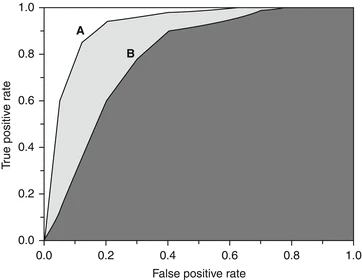
\includegraphics[width=0.5\linewidth]{images//Capitolo3/Curva ROC.png}
        \caption{Curva ROC}
        \label{fig:Curva ROC}
    \end{figure}
    
    \item \textbf{Area sottesa alla curva Precisione-Richiamo (AUC\textunderscore PR)}: rappresenta un semplice modo per sintetizzare le prestazioni generali di un modello, più alto è il valore più alto sarà il numero di predizioni corrette. La curva Precision-Recall è utile quando la classe positiva è rara, perché si concentra sulla capacità del modello di identificare correttamente i casi positivi, senza essere influenzata dai veri negativi.
\end{itemize}
In queste formule per il calcolo delle metrica abbiamo usato: TP per rappresentare i veri positivi, ossia i segmenti delle telemetrie correttamente identificati come anomalie; TN per i veri negativi, cioè segmenti correttamente identificati come nominali ossia regolari; FP per i falsi positivi, ossia i segmenti erratamente classificati anomalie e FN per i falsi negativi che rappresentano i segmenti erratamente classificati come non anomalie.
Tutte le metriche descritte possono assumere valori tra $[0,1]$, tranne MCC che assume valori tra $[-1,1]$.
Tutte le metriche però più si avvicinano ad uno e più il modello testato risulta efficace, rispetto ad uno con valori inferiori delle stesse.

Le metriche appena viste ci serviranno successivamente per valutare le capacità degli algoritmi avendo un metro di paragone unico per tutti i modelli.
Tra gli obbiettivi resta comunque cercare di non sovraccaricare il processore del satellite, mantenendo quindi la complessità del modello abbastanza bassa.
Nell'eventualità di una piccola perdita di efficacia, ma con un grande risparmio in complessità del modello, viene ovviamente premiata l'efficienza.

\chapter{Datasets}
Procediamo ora a descrivere i dataset contenenti dati di telemetrie registrati negli anni e resi pubblici in modo da poter sperimentare e migliorare gli algoritmi già presenti.

\section{Dataset ESA}

Il dataset di riferimento più importante per la rilevazione delle anomalie è quello fornito dall'ESA (European Space Agency) che conta dati di tre missioni. Di queste solo i dati di due vengono utilizzati per creare il benchmark, per le caratteristiche dell'insieme di dati; infatti in \textit{"Mission 3"} abbiamo: poche anomalie e per lo più banali, un gran numero di buchi di comunicazione e segmenti non validi.

Nell'articolo$^{\text{\cite{ESA_benchmark}}}$ in questione i dati satellitari grezzi di \textit{"Mission 1"} e \textit{"Mission 2"} vengono preprocessati per renderli uniformi e quindi utilizzabili con la maggior parte degli algoritmi.

In questa fase è stato utilizzato lo strumento OXI$^{\text{\cite{OXI_annotation_tool}}}$ per l'etichettatura collaborativa dei dati da cui si è potuto estrarre delle telemetrie che rappresentano periodi di funzionamento nominale e anomalo. Tutti i dati sono stati sottoposti ad una doppia fase di etichettatura e controllo.

I canali sono divisi tra "target" e "non target", dove quest'ultimi sono usati per gli algoritmi solo come informazioni addizionali. Un canale target, quello usato per rilevare le anomalie, è diviso in gruppi di dati con caratteristiche simili così da rendere più facile per l'algoritmo processarli ed interpretarli e, nel caso, allenarlo solo su quel gruppo specifico.
\pagebreak

\begin{table}[h!]
    \centering
    \begin{tabular}{|l|c|c|}
        \hline
         \textbf{}& \textbf{Mission 1} & \textbf{Mission 2}\\
         \hline
        \textbf{Channels} & 76 & 100\\
        Target/Non target & 58/18 & 47/53\\
        \hline
        \textbf{Telecommands} & 698 & 123\\
        \hline
        \textbf{Annotate Events} & 200 & 644 \\
        Anomalies& 118 & 31\\
        Rare Nominal Events &78  & 613\\
        Univariate/Multivariate& 32/164 & 9/635\\
        \hline
    \end{tabular}
    \caption{Configurazione Dataset ESA}
    \label{tab:costituzioneESA_dataset}
\end{table}

Possiamo osservare dalla Tabella \ref{tab:costituzioneESA_dataset} che la densità di anomalie in termini di punti di dati annotati, varia tra $0,57\%$ per la \textit{"Mission 2"} e $1,80\%$ per la \textit{"Mission 1"} questo va a confermare un'impronta più realistica rispetto ai dataset meno recenti che avevano una densità di anomalie estremamente più alta ed irrealistica.

\section{Dataset NASA}
Il dataset NASA riporta i dati provenienti da missioni reali effettuate negli anni, questi coprono più aspetti relativi al contesto spaziale con il conseguente aumento di complessità.

Il dataset contiene serie temporali con numerosi parametri di telemetria, tra cui eventi normali e anomali.
Le anomalie sono rare, infatti possiamo riscontrare canali che non ne possiedono nemmeno una, rappresentando una sfida significativa, insieme anche al fatto che non tutti i dati sono etichettati.

Elenchiamo alcune particolarità e soprattutto sfide:
\begin{itemize}
    \item Rarità: le anomalie presenti nel dataset sono in quantità ridotta, rendendo l'addestramento dei modelli più difficile;
    \item Etichettatura: le etichettature dei dati sono incomplete, complicando ulteriormente l'identificazione;
    \item Rumorosità: i dati presenti, a causa anche della provenienza da diverse missioni, contengono lacune e sono spesso rumorosi a causa di fattori esterni;
    \item Variabilità: i parametri variano molto;
    \item Veridicità: i dati rispecchiano la realtà, portando così a poter testare i modelli in un contesto simile ai dati reali.
\end{itemize}

Utilizziamo questo dataset perché permette di utilizzare dati realistici, valutando in maniera più accurata gli algoritmi proposti. Inoltre, utilizzare un dataset con molteplici sperimentazioni e test effettuati, permette di avere un confronto diretto dei modelli, potendo anche validare i risultati ottenuti, aumentando la credibilità e avvalorando le analisi proposte da altri o la possibilità che altri validino le nostre.

\section{Motivazioni}
Il dataset ESA precedentemente descritto porta alla risoluzione di vari problemi noti nell'ambito della rilevazione di anomalie.
Il primo problema, relativo al dataset NASA, è la loro struttura, come si evidenzia nei dataset \textit{NASA Soil Moisture Active Passive} (SMAP) e  \textit{Mars Science Laboratory} (MSL), i quali offrono brevi frammenti di segnali e comandi correlati da, rispettivamente, 55 e 27 parametri di telemetria, con un totale di 105 anomalie annotate; infatti abbiamo una densità di anomalie irrealistica, alto numero di anomalie banali, verità di base etichettate in maniera errate ed una mancanza di correlazione tra comandi e canali. 
% Come conseguenza di questo è stato deciso che questi dataset non andrebbero usati per il benchmarking del rilevamento delle anomalie.
Il secondo problema invece rappresenta la mancanza di annotazione di eventi anomali, alcuni esempi sono gli insiemi di dati di \textit{Mars Express6} e \textit{NASA WebTCAD7}.

Il dataset ESA risolve i problemi elencati, ma nasce come dataset di missioni su larga scala, le quali sono molto complesse e stabili, portando con sé problemi non più relativi alla distribuzione delle anomalie, ma improntati verso difficoltà di esecuzione e potenza di calcolo.

Il dataset che introdurremo successivamente è concettualmente diverso, infatti affronta una missione ESA OPS\textunderscore SAT molto semplificata, al fine di renderne più accessibile l'uso, oltre ad essere di dimensione considerevolmente minore.

Questo processo di apertura è reso anche tramite la sostituzione giornaliera dell'intero sistema software fino al sistema operativo del satellite, così da consentire ai ricercatori di caricare il proprio software a bordo del satellite. Per implementare questa funzionalità venne usato FDIR$^{\text{\cite{FDIR}}}$ (Fault Detection, Isolation, and Recovery), un metodo che rileva, isola e corregge automaticamente i malfunzionamenti, assicurando il funzionamento continuo del satellite e permettendo una gestione dinamica delle sue funzionalità.

Le telemetrie grezze sono caratterizzate da molte lacune nei dati ed altre imprecisioni, queste vengono curate da ingegneri ed esperti nei modelli di apprendimento automatico per rendere l'insieme di dati fruibile alla creazione di tecniche di rilevamento delle anomalie basate su di essi.
Una di queste modifiche è la seguente:

\begin{quote}
    Selezione e annotazione di verità di base (ground\textunderscore truth) di 2123 brevi frammenti di telemetria a canale singolo, ossia serie temporali univariate$^{\text{\cite{OPS-SAT}}}$, registrate in 9 canali di telemetria.
\end{quote}

Infine questo dataset, con il relativo benchmark e tutti i dati disponibili al suo interno, è stato messo a disposizione per aiutare la comunità nella ricerca di nuovi approcci per la rilevazione delle anomalie, confrontandosi tra di loro in modo imparziale ed equo, così da affrontare anche il problema della riproducibilità nell'ambiente dell'apprendimento automatico (dato che i dataset sono uniformati, l'ambiente di esecuzione potrebbe essere diverso e sono state utilizzate varie metriche). 

Tutto ciò che è stato sviluppato con l'aiuto del dataset verrà convalidato con il lancio alla fine del 2025 del satellite successore OPS\textunderscore SAT VOLT (dopo aver distribuito i vari modelli a bordo del satellite).


\section{OPS-SAT Dataset}
Nel dataset OPS\textunderscore SAT sono contenuti i dati delle telemetrie del satellite OPS\textunderscore SAT dell'ESA (Figura \ref{fig:OP-SAT_satellite}). Questo satellite di tipo CubeSat aveva dimensione 3 unità (3U dove 1U=10cm$^3$); esso ormai non è più in orbita, era stato lanciato a Dicembre del 2019 con lo scopo di dimostrare l'elaborazione dei dati in orbita e di generare dati utili come immagini satellitari e telemetrie.

\begin{figure}[ht]
    \centering
    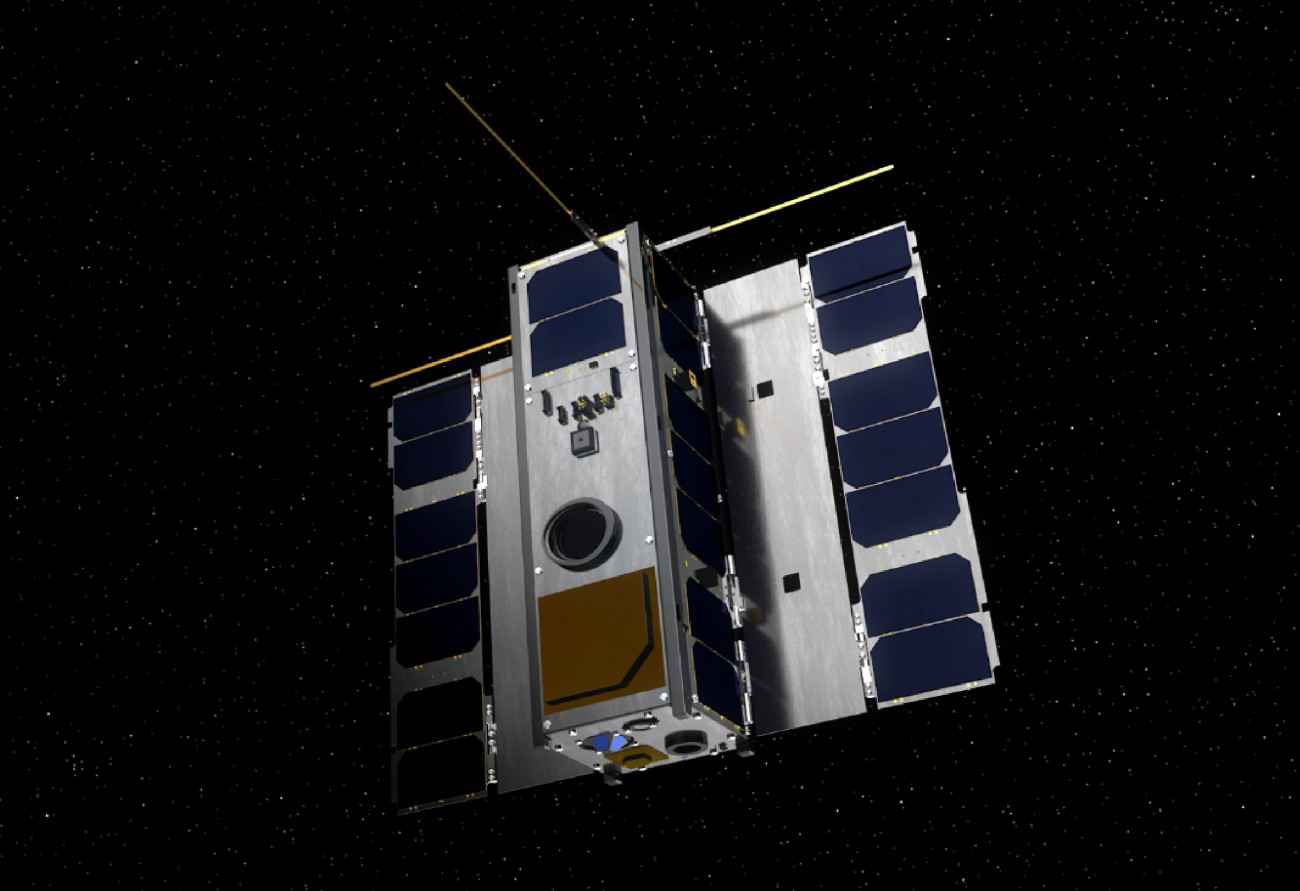
\includegraphics[width=0.5\linewidth]{images/Capitolo2/OP-SAT_satellite.png}
    \caption{Satellite OPS\textunderscore SAT. Fonte: European Space Agency}
    \label{fig:OP-SAT_satellite}
\end{figure}

Come nel dataset precedente anche qui i dati hanno bisogno di essere preprocessati per renderli fruibili alla maggior parte degli algoritmi (OXI$^{\text{\cite{OXI_annotation_tool}}}$). In questo caso sono state progettate 18 caratteristiche per l'attività di rilevamento delle anomalie, ossia sono stati estratti tratti significativi dai dati. Questo processo è chiamato Feature Extraction e serve per ridurre la complessità dei dati in ingresso, rendendoli più significativi.

Tutti i segmenti ricavati rappresentano le sfide che dobbiamo affrontare con i dati delle telemetrie, ognuno di questi è composto da:
\begin{itemize}
    \item $\langle$\texttt{timestamp}$\rangle$: rappresenta il marcatore temporale nel momento della registrazione;
    \item $\langle$\texttt{channel}$\rangle$: è il nome del canale;
    \item $\langle$\texttt{value}$\rangle$: è il valore del segnale acquisito;
    \item $\langle$\texttt{label}$\rangle$: rappresentano le annotazioni certe, quelle annotate manualmente;
    \item $\langle$\texttt{segment}$\rangle$: rappresenta il numero consecutivo del segmento;
    \item $\langle$\texttt{sampling}$\rangle$: è il tasso di campionamento;
    \item $\langle$\texttt{train}$\rangle$: indica se il segmento appartiene al training set.
    
\end{itemize}

Il dataset è stato diviso in una parte di allenamento, Training Set ($T$), ed una di test, Test Set ($\Psi$). Questi rappresentano rispettivamente i dati usati per l'allenamento del modello e i dati usati per fare le valutazioni delle performance dell'algoritmo.

\begin{table}[h!]
    \centering
    \begin{tabular}{|l|c|c|c|}
        \hline
        \textbf{Classi} &\textbf{Training Set} ($T$) & \textbf{Test Set ($\Psi$)}&\textbf{Total} \\
        \hline
         Nominali& 1273&416 &1689 \\
         Anomalie& 321&529 &434\\
         \hline
    \end{tabular}
    \caption{Composizione Dataset OPS\textunderscore SAT}
    \label{tab:dataset_op-sat}
\end{table}

Le classi mostrate in Tabella \ref{tab:dataset_op-sat}, nominali e anomalie, rappresentano rispettivamente segmenti che rispettano valori normali o attesi e segmenti invece che superano questi valori o discordano dai valori attesi.

Partendo dai benchmark effettuati su NASA ed OPS\textunderscore SAT, analizzeremo le metriche e le prestazioni utilizzando vari modelli per il rilevamento delle anomalie, partendo dal secondo dataset (OPS\textunderscore SAT), che contiene dati più semplici per il nostro obiettivo, per poi dedicarci a NASA per finire.

\section{Validazione Paper OPS\textunderscore SAT}
In questa sezione vogliamo verificare le prestazioni di tutti gli algoritmi presenti nel paper relativo ad OPS\textunderscore SAT, questo per avere un confronto con le metriche risultanti degli algoritmi che vedremo successivamente.

I dati che utilizziamo sono estratti tramite le funzioni rese disponibili dal paper, partendo quindi già con i dati elaborati e divisi in \texttt{X\textunderscore train, X\textunderscore test, y\textunderscore train, y\textunderscore test}.
Tramite la funzione \texttt{StandardScaler()} scaliamo i dati, ottenendo le metriche desiderate, riportate nella tabella sottostante.
\vspace{0.5cm}
\begin{table}[h]
    \centering
    \begin{adjustbox}{max width=\textwidth}
        \begin{tabular}{|c|c|c|c|c|c|c|c|c|}
        \hline
            \textbf{Modello} & \textbf{Accuracy} &\textbf{Precision}  & \textbf{Recall} & \textbf{F1} & \textbf{MCC} & \textbf{AUC-PR} & \textbf{AUC-ROC} & \textbf{N-Score}\\
            \hline
            \multicolumn{9}{|c|}{\textbf{Supervised}} \\
            \hline
            \textbf{LinearSVC} & 0.926 & 0.911 & 0.726 &0.808  & 0.771 & 0.949 & 0.976 &0.867 \\
            \hline
             \textbf{LogisticRegression}& 0.924 & 0.92 & 0.708 & 0.8 & 0.764 & 0.949 & 0.976 & 0.867 \\
             \hline
             \textbf{FCNN}& 0.96 & 0.926 & 0.885 & 0.905 & 0.88 & 0.963 & 0.982 & 0.903 \\
             \hline
             \textbf{AdaBoost}& 0.934 & 0.89 & 0.788 & 0.836 & 0.797 & 0.923 & 0.962 & 0.841 \\
             \hline
             \textbf{RF+ICCS}& 0.964 &\textbf{ 0.98} & 0.85 & 0.91 & 0.891 & 0.949 & 0.976 & 0.867 \\
             \hline
             \textbf{Linear+L2}& 0.902 & 0.969 & 0.558 & 0.708 & 0.69 & 0.889 & 0.95 & 0.814 \\
             \hline
             \textbf{XGBOD}& \textbf{0.968} & 0.953 & \textbf{0.894} & \textbf{0.922} & \textbf{0.903} & \textbf{0.969} & \textbf{0.99} & \textbf{0.912} \\
             \hline
             \multicolumn{9}{|c|}{\textbf{Unsupervised}} \\
             \hline
             \textbf{MO-GAAL} & \textbf{0.896 }& 0.939 & 0.549 &\textbf{0.693}  & \textbf{0.669} & \textbf{0.771} & 0.849 &0.699 \\
        \hline
         \textbf{AnoGAN}& 0.594 & 0.296 & \textbf{0.655} & 0.408 & 0.19 & 0.403 & 0.651 & 0.239 \\
         \hline
         \textbf{SO-GAAL}& 0.89 & 0.937 & 0.522 & 0.67 & 0.649 & 0.858 & \textbf{0.919} & \textbf{0.761} \\
         \hline
         \textbf{IForest}& 0.701 & 0.297 & 0.292 & 0.295 & 0.105 & 0.347 & 0.635 & 0.301 \\
         \hline
         \textbf{KNN}& 0.849 & 0.78 & 0.407 & 0.535 & 0.489 & 0.658 & 0.852 & 0.593 \\
         \hline
         \textbf{OCSVM}& 0.837 & 0.721 & 0.389 & 0.506 & 0.447 & 0.659 & 0.788 & 0.655 \\
         \hline
         \textbf{ABOD}& 0.845 & 0.782 & 0.381 & 0.512 & 0.472 & 0.644 & 0.843 & 0.584 \\
         \hline
         \textbf{INNE}& 0.83 & 0.689 & 0.372 & 0.483 & 0.418 & 0.624 & 0.801 & 0.646 \\
         \hline
         \textbf{ALAD}& 0.819 & 0.667 & 0.301 & 0.415 & 0.361 & 0.537 & 0.7 & 0.451 \\
         \hline
         \textbf{LMDD}& 0.822 & \textbf{1.0} & 0.168 & 0.288 & 0.37 & 0.624 & 0.765 & 0.663 \\
         \hline
         \textbf{SOD}& 0.826 & 0.611 & 0.513 & 0.558 & 0.453 & 0.621 & 0.797 & 0.549 \\
         \hline
         \textbf{COF}& 0.834 & 0.667 & 0.442 & 0.532 & 0.449 & 0.603 & 0.774 & 0.593 \\
         \hline
         \textbf{LODA}& 0.83 & 0.689 & 0.372 & 0.483 & 0.418 & 0.549 & 0.692 & 0.522 \\
         \hline
         \textbf{LUNAR}& 0.819 & 0.743 & 0.23 & 0.351 & 0.313 & 0.541 & 0.797 & 0.46 \\
         \hline
         \textbf{CBLOF}& 0.802 & 0.569 & 0.292 & 0.386 & 0.304 & 0.45 & 0.574 & 0.372 \\
         \hline
         \textbf{DIF}& 0.788 & \textbf{1.0} & 0.009 & 0.018 & 0.084 & 0.494 & 0.805 & 0.522 \\
         \hline
         \textbf{VAE}& 0.794 & 0.532 & 0.292 & 0.377 & 0.283 & 0.446 & 0.687 & 0.513 \\
         \hline
         \textbf{GMM}& 0.783 & 0.482 & 0.239 & 0.32 & 0.225 & 0.426 & 0.713 & 0.389 \\
         \hline
         \textbf{DeepSVDD}& 0.788 & 0.509 & 0.239 & 0.325 & 0.241 & 0.344 & 0.55 & 0.336 \\
         \hline
         \textbf{PCA}& 0.779 & 0.464 & 0.23 & 0.308 & 0.21 & 0.373 & 0.612 & 0.363 \\
         \hline
         \textbf{COPOD}& 0.767 & 0.4 & 0.177 & 0.245 & 0.147 & 0.328 & 0.627 & 0.257 \\
         \hline
         \textbf{SOS}& 0.758 & 0.364 & 0.177 & 0.238 & 0.125 & 0.308 & 0.524 & 0.274 \\
         \hline
         \textbf{ECOD}& 0.767 & 0.396 & 0.168 & 0.236 & 0.14 & 0.34 & 0.637 & 0.345 \\
         \hline
        \end{tabular}
    \end{adjustbox}
    \caption{Risultati esecuzione di tutti gli algoritmi del benchmark OPS\textunderscore SAT}
    \label{tab:tabella_inizialeOPS_SAT}   
\end{table}
\section{XGBOD}
% Scrivere introduzione all'analisi di XGBOD come stato dell'arte
Partendo dai risultati ottenuti per la validazione del paper OPS\textunderscore SAT, prendiamo in analisi il modello XGBOD, per poter effettuare un confronto con le metodologie che proporremo successivamente effettuando test e analizzando i risultati ottenuti.

XGBOD (eXtreme Gradient Boosting for Outlier Detection) è un algoritmo composto da tre fasi:
\begin{enumerate}
    \item Generazione di nuove rappresentazioni di dati: vengono applicati vari metodi di rilevamento di anomalie non supervisionati ai dati originali, per ottenere punteggi di anomalie, questi rappresentano la nuova vista dei dati;
    \item Selezione dei punteggi rilevanti: i punteggi ottenuti nella fase precedente vengono filtrati per usare solo quelli utili, quest'ultimi sono combinati con le caratteristiche iniziali, creando un nuovo spazio delle caratteristiche arricchito;
    \item Addestramento del modello XGBoost: viene addestrato il modello XGBoost su questo nuovo spazio delle caratteristiche e le previsioni che otteniamo determinano se ogni dato è un'anomalia o no.
\end{enumerate}
Utilizziamo XGBOD invece che XGBoost direttamente perché quest'ultimo, essendo un modello supervisionato, ha bisogno di dati etichettati e soprattutto con anomalie rare, non facili da etichettare.

XGBOD aggiunge una parte di preprocessing, aumenta le informazioni del set di dati con punteggi di anomalie ed utilizza metodi di rilevamento non supervisionato come Isolation Forest, Local Outlier Factor, ecc..

\subsection{XGBoost}
Il modello XGBoost di tipo supervisionato, si sviluppa con un processo iterativo di addestramento di alberi decisionali deboli (alberi decisionali poco profondi e quindi poco accurati), questi vengono combinati tra di loro portando un miglioramento progressivo delle prestazioni del modello.

XGBoost è composto da pochi passi ma ripetuti iterativamente: come primo passo vengono calcolati i residui, la differenza tra le previsioni iniziali ed i valori reali; questi sono i valori che vogliamo ridurre. Con questi valori il modello addestra un insieme di alberi decisionali deboli, dove ognuno cerca di correggere questi valori migliorando le previsioni del modello precedente. Tutti gli alberi vengono aggiunti al modello complessivo di XGBoost, che aggiorna le sue previsioni combinando tutti gli alberi precedentemente costruiti.

Per regolare tutto questo processo, sono applicate internamente tecniche di limitazione e regolazione per evitare un overfitting del modello. All'interno di XGBoost è presente anche una metrica chiamata \textit{tasso di apprendimento}, che permette di decidere quanto un albero incide sul risultato finale, minimizzando così gli errori di percorso.

\subsection{Risultati ottenuti}
Qui sono elencati i risultati ottenuti effettuando varie prove con parametri diversi per ottimizzare XGBOD ed ottenere il miglior compromesso tra efficienza ed efficacia.
\vspace{0.4cm}
\begin{table}[h!]
    \centering
    \begin{adjustbox}{max width=\textwidth}
        \begin{tabular}{|c|c|c|c|c|c|c|c|c|c|}
        \hline
        \textbf{Modello} & \textbf{Accuracy} &\textbf{Precision}  & \textbf{Recall} & \textbf{F1} & \textbf{MCC} & \textbf{AUC-PR} & \textbf{AUC-ROC} & \textbf{Nscore} & \textbf{Tempo}\\
     \hline
            \textbf{M+P} & \textbf{0.97} & 0.945 & \textbf{0.912} &\textbf{0.928}  & \textbf{0.909} & 0.973 & 0.992 &0.92 & \textbf{1.5s}\\
            \hline
             \textbf{Early}& \textbf{0.97} & 0.971 & 0.885 & 0.926 & \textbf{0.909} & 0.969 & 0.99 & 0.912 & 11.3s\\
             \hline
             \textbf{+M}& 0.968 & 0.944 & 0.903 & 0.923 & 0.903 & 0.974 & 0.91 & 0.92 & 3.3s\\
             \hline
             \textbf{P}& 0.964 & 0.943 & 0.885 & 0.913 & 0.891 & 0.972 & \textbf{0.991} & 0.912 &9.8s\\
             \hline
             \textbf{Senza P}& 0.962 & 0.935 & 0.885 & 0.909 & 0.886 & \textbf{0.977} & 0.992 & 0.912 &9.7s\\
             \hline
             \textbf{Grid}& 0.947 & \textbf{0.989} & 0.761 & 0.86 & 0.839 & 0.898 & 0.945 & \textbf{0.969} &45.9s \\
             \hline
        \end{tabular}
    \end{adjustbox}
    \caption{Prove esecuzione di XGBOD}
    \label{tab:XGBOD_table}
\end{table}
\pagebreak

LEGENDA:
\begin{itemize}
    \item M+P: indica l'utilizzo di più modelli, oltre a quelli utilizzati di default,   combinati all'uso di parametri, questo per migliorare le prestazioni complessive;
    \item Grid: è una tecnica che esplora tutte le possibili combinazioni di iperparametri predefiniti (n\textunderscore estimators, max\textunderscore depth e learning\textunderscore rate) per trovare la configurazione che restituisce i migliori risultati;
    \item EarlyStop: viene utilizzato un meccanismo di EarlyStop che ferma l'esecuzione dell'algoritmo quando gli iperparametri non migliorano più per un numero definito di cicli.
\end{itemize}

Dalla Tabella \ref{tab:XGBOD_table} possiamo vedere che il miglior risultato è quello che utilizza più modelli per l'addestramento ed i parametri modificati al fine di efficientare l'esecuzione. Oltre ad avere degli ottimi risultati, l'esecuzione rimane praticamente istantanea sul nostro dataset di esempio OPS\textunderscore SAT.
\chapter{ ROCKET: RandOm Convolutional KErnel Transform}
In questo capitolo andremo ad analizzare gli algoritmi di nostro interesse, ossia ROCKET e ROCKAD.
Questi algoritmi lavorano con le timeseries, le quali sono una sequenza di dati registrati ad intervalli di tempo consecutivi. Ogni punto della serie è associato ad un timestamp, il quale indica il momento in cui è stato registrato.

ROCKET, ancora non utilizzato per il rilevamento delle anomalie, è stato selezionato come nuovo algoritmo, per la sua grande capacità di estrarre caratteristiche importanti dalle serie temporali e per l'efficienza di utilizzo.
Tutto questo è reso possibile grazie anche ai kernel casuali che non necessitano di grande capacità di calcolo, rispetto ad altri algoritmi più complessi.

Ciò che garantisce la robustezza di ROCKET sono i kernel casuali e le tecniche di pooling che vi si possono applicare, portando così a poter eliminare la necessità di ottimizzare gli iperparametri.
ROCKET viene descritto come efficiente e scalabile anche su grandi dataset, oltre ad un fattore di adattabilità ai dataset con caratteristiche variabili, molto elevato.

L'obbiettivo principale è utilizzare ROCKET per il rilevamento delle anomalie direttamente a bordo dei satelliti, riducendo la necessità di scambiare informazioni con la stazione centrale e minimizzando i falsi positivi.

Dopo l'uscita di ROCKET e valutata la sua efficacia è stato introdotto ROCKAD (Random Convolutional Kernel Transform Anomaly Detector), questo è un estensione di ROCKET progettata appositamente per il rilevamento delle anomalie.

Secondo gli sviluppatori, ROCKAD permette di ottenere un rilevamento di anomalie più preciso e mirato, sfruttando le caratteristiche estratte da ROCKET.
ROCKAD trova maggiore spazio in contesti in cui l'etichettatura dei dati è limitata o assente (come vedremo per NASA), consentendo una classificazione basata su punteggi di anomalia.

\section{ROCKET}
ROCKET è un algoritmo convoluzionale, questo è anche detto rete neurale convoluzionale (CNN). Questi algoritmi lavorano su dati con una struttura a griglia come immagini e serie temporali e sono progettati per riconoscere pattern all'interno dei dati tramite operazioni di convoluzione.
Vengono utilizzati i kernel\footnote{Matrice di pesi usata per eseguire operazioni di filtraggio per estrarre caratteristiche specifiche, opera tramite moltiplicazioni e addizioni}, che operando sui dati in input estraggono caratteristiche locali dei dati (features); in questa fase possono essere applicate tecniche di centratura, ovvero aggiungere dei bordi attorno all'input, così da mantenere le dimensioni dopo aver applicato il kernel, questo si chiama padding.

Ci sono tecniche applicabili a ROCKET come il pooling, che ha lo scopo di ridurre la dimensione e quindi di rendere l'algoritmo meno sensibile alle traslazioni. In merito a questo vediamo le due tecniche più utilizzate:
\begin{itemize}
    \item Max Pooling: prende solo il valore massimo in una finestra specifica riducendo la dimensione dell'input;
    \item Average Pooling: riduce la dimensione prendendo la media dei valori in una finestra;
    \item Proportion of Positive Value (PPV): calcola la percentuale di valori positivi nell'output della convoluzione, individuando quanto spesso il kernel produce valori maggiori di zero.
\end{itemize}

In conclusione abbiamo il passaggio per gli strati: i dati vengono appiattiti (flattening) fatti passare attraverso uno o più strati completamente connessi per la classificazione o la regressione, in modo da ottenere il risultato desiderato.

ROCKET in particolare utilizza i kernel convoluzionali casuali, generandone un gran numero con iperparametri scelti casualmente, come lunghezza del kernel, Dilatation Rate, Bias e pesi dei kernel.
Questi kernel filtrano i dati delle serie temporali producendo una serie di features. Utilizzando tecniche di pooling viste in precedenza, otteniamo statistiche riassuntive da queste features.
La procedura viene ripetuta per tutti i kernel, portando ad un enorme quantità di caratteristiche e quindi una maggiore possibilità di estrarre tutti i pattern comuni.

Le caratteristiche estratte vengono poi date in input ad algoritmi di classificazione, tipicamente una regressione logistica data la sua scalabilità e velocità su grandi dataset.
L'algoritmo viene addestrato su questi elaborati per effettuare la classificazione delle serie temporali.

Per rendere più chiara la logica di funzionamento prendiamo in considerazione la Figura \ref{fig:rocket_paper}, presa dal paper di ROCKAD$^{\text{\cite{rockad_paper}}}$.
Come possiamo osservare, in ingresso ROCKET prende la timeseries di una specifica features $T$, e tramite moltiplicazioni tra matrici, chiamate filtri (kernel), otteniamo un array di caratteristiche di $2K$ features ($K$ features per ogni tecnica di pooling utilizzata).
Questo processo viene ripetuto per ogni features del dataset, portando ad avere un numero di caratteristiche pari a 10.000 volte il numero di features iniziali (nel caso di kernel di default).

\begin{figure}[!ht]
    \centering
    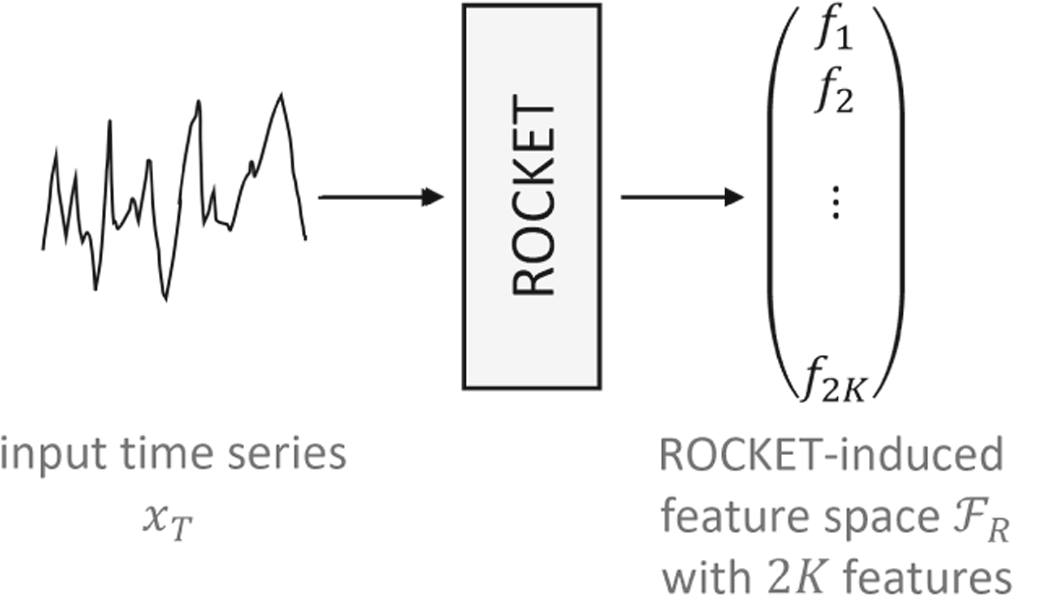
\includegraphics[width=0.5\linewidth]{images//Capitolo4/ROCKET_Paper.png}
    \caption{Funzionamento ROCKET}
    \label{fig:rocket_paper}
\end{figure}

ROCKET quindi scorre la timeseries con delle finestre di dimensione uguale tra loro, come possiamo vedere dalla Figura \ref{fig:rocket_finestre}. Le caratteristiche estratte da ciascuna finestra vengono successivamente utilizzate da un classificatore, che elabora tali informazioni per fornire una predizione sull'intera serie temporale relativa alla feature originale.

\begin{figure}[!ht]
    \centering
    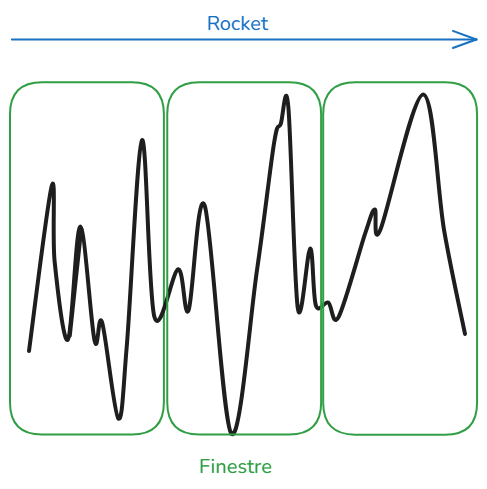
\includegraphics[width=0.5\linewidth]{images//Capitolo4/ROCKET_finestre.png}
    \caption{Finestre ROCKET su timeseries}
    \label{fig:rocket_finestre}
\end{figure}
\pagebreak
\subsection{Aspetti Tecnici}
Per implementare ROCKET abbiamo usato la libreria utilizzata anche dal paper di ROCKAD tramite:
\begin{lstlisting}[language=Python]
from sktime.transformations.panel.rocket import Rocket
\end{lstlisting}
I parametri più importanti sono:
\begin{itemize}
    \item Numero di kernel (num\textunderscore kernels): rappresenta il numero di kernel casuali da generare, il valore predefinito è 10.000, un numero maggiore di kernel tende a migliorare l'accuratezza della classificazione, di conseguenza aumenta la complessità e quindi il tempo di calcolo;
    \item Lunghezza del kernel (input\textunderscore length): rappresenta la lunghezza del singolo kernel, questa è casuale e determina quanto, della serie temporale, viene considerato durante la convoluzione;
    \item Dilatazione: è un parametro che controlla la distanza tra i punti analizzati nel kernel; ROCKET usa varie dilatazioni per catturare caratteristiche di diverse scale temporali;
    \item Padding: determina come vengono gestiti i bordi delle serie temporali durante la fase di convoluzione.
\end{itemize} 

I vantaggi di ROCKET sono:
\begin{itemize}
    \item Efficienza computazionale elevata: è progettato per essere estremamente veloce e scalabile in modo che possa gestire grandi dataset in tempi ristretti;
    \item Robustezza: dato che si basa su kernel casuali, consente di generalizzare bene su nuovi problemi, senza la necessità di perfezionare gli iperparametri;
    \item Semplicità: ROCKET permette di usare un solo iperparametro, ossia il numero di kernel, riducendo così la complessità associata al perfezionamento rispetto ad altri metodi di classificazione delle serie temporali.
\end{itemize}
\subsection{Metodologia Applicata}
Nel paper di ROCKET$^{\text{\cite{paper_rocket}}}$, esso viene applicato, in particolare per la classificazione delle serie temporali, portando a sostegno molteplici valutazioni su dataset di BakeOff. Partendo da queste analisi e valutazioni del modello sulle serie temporali vogliamo riprodurre tali dati, molto promettenti, per la prima volta utilizzando ROCKET con lo scopo di classificazione delle anomalie sulle serie temporali.

% ================ Da vedere come e se scrivere in base a mail e funzionamento
Un aspetto da considerare è la formattazione dei dati che utilizziamo, infatti estraendo i dati dal dataset grezzo di OPS\textunderscore SAT e elaborandoli, come vedremo meglio nella parte relativa a ROCKAD, in modo che siano compatibili con ROCKET.

\subsection{Test Effettuati}
Come primo aspetto abbiamo eseguito in locale gli esperimenti del paper di ROCKET per avere una validazione empirica dell'algoritmo, ottenendo risultati compatibili con quelli della tabella del paper$^{\text{\cite{paper_rocket}}}$; successivamente abbiamo testato la nostra implementazione sui medesimi dataset ottenendo i risultati della Tabella \ref{tab:Rocket_paper}.
\begin{table}[h!]
    \centering
    \begin{adjustbox}{max width=\textwidth}
        \begin{tabular}{|c|c|}
            \hline
            \textbf{Dataset} & \textbf{Accuracy}\\
            \hline
             Coffee &1.0 \\
             \hline
             Computers& 0.64\\
             \hline
             Adiac& 0.634\\
             \hline
             ArrowHead& 0.788\\
             \hline
             BeetleFly& 0.8\\
             \hline
             CinCECGTorso& 0.7898\\
             \hline
             CBF& 0.971\\
             \hline
             ChlorineConcentration& 0.590\\
             \hline
             GunPoint& 0.9866\\
             \hline
             Ham& 0.771\\
             \hline
             HandOutlines& 0.935\\
             \hline
             InlineSkate& 0.367\\
             \hline
             Lightning2& 0.623\\
             \hline
             Mallat& 0.928\\
             \hline
             MiddlePhalanxTW& 0.558\\
             \hline
        \end{tabular}
    \end{adjustbox}
    \caption{Esecuzione di ROCKET su dataset "BakeOff"}
    \label{tab:Rocket_paper}
\end{table}
\pagebreak

Nei risultati che osserveremo in seguito nella Tabella \ref{tab:RocketOPS_SAT}, sono state effettuate molte prove con varie modalità.
La prima è unsupervised, ovvero utilizziamo ROCKET per estrarre una grande quantità di caratteristiche e, tramite una threshold, fare una classificazione binaria senza aver effettuato un training con le etichette dei risultati.
Una threshold è una soglia, che indica il valore di riferimento per decidere quando una predizione deve essere classificata come positiva o negativa, in questo caso segnala quando un valore deve essere considerato o no anomalo.
La seconda modalità che abbiamo osservato è supervised, effettuando quindi il training sulle features trovate da ROCKET passando però le etichette delle classificazioni.
Per questo abbiamo utilizzato vari algoritmi supervised per analizzare le varie performance e trovare il migliore.
Abbiamo anche osservato una modalità ibrida, ossia al posto dell'utilizzo di una threshold o un algoritmo supervised abbiamo puntato su uno unsupervised (KNN) facendo il training sulle features e restituendo delle prediction e delle classificazioni; il KNN, solitamente usato in modo supervised, nel nostro caso è stato utilizzato per calcolare la distanza dai $k$ vicini più prossimi e assegnando un punteggio di anomalia basato su queste distanze.

\texttt{RidgeClassifierCV}: è il modello di classificazione usato come standard nel paper di ROCKET; nel nostro caso utilizzandolo con il dataset OPS\textunderscore SAT abbiamo riscontrato metriche migliori in tutti i test.
\begin{table}[h!]
    \centering % Correttamente posizionato
    \begin{adjustbox}{max width=\textwidth}
        \begin{tabular}{|c|c|c|c|c|c|c|c|c|c|}
        \hline
        \textbf{Modalità} & \textbf{Accuracy} &\textbf{Precision}  & \textbf{Recall} & \textbf{F1} & \textbf{MCC} & \textbf{AUC-PR} & \textbf{AUC-ROC} & \textbf{NScore}&\textbf{Tempo}\\
        \hline
        \multicolumn{10}{|c|}{\textbf{Unsupervised}} \\
        \hline
        \textbf{Threshold} & 0.546 & \textbf{1.0} & 0.048 &0.092  & 0.161 & 0.46 & 0.468 & 0.419 &7s \\
        \hline
        \multicolumn{10}{|c|}{\textbf{Supervised}} \\
        \hline
         \textbf{RidgeCV} &\textbf{ 0.777} & 0.704 & \textbf{0.919} &\textbf{0.797}  & \textbf{0.584} & 0.787& 0.829 &0.726&6.6s \\
        \hline
        \textbf{LogisticReg} & \textbf{0.777} & 0.704 & \textbf{0.919} &\textbf{0.797}  &\textbf{ 0.584} & 0.773& 0.837 &\textbf{0.774} &53.3s\\
        \hline
        \textbf{RidgeReg} & 0.538 & \textbf{1.0} & 0.032 &0.062  & 0.131 & \textbf{0.779}& \textbf{0.844} &0.758 &5.8s \\
        \hline
        \multicolumn{10}{|c|}{\textbf{Ibrid Unsupervised}} \\
        \hline
        \textbf{KNN} & 0.531 & 0.6 & 0.048 &0.09  & 0.049 & 0.407& 0.294 &0.29 & 9.4s \\
        \hline
        \end{tabular}
    \end{adjustbox}
    \caption{Algoritmi eseguiti su dataset OPS\textunderscore SAT}
    \label{tab:RocketOPS_SAT}
\end{table}


\pagebreak

\subsection{Implementazione}

Riportiamo qui il codice dell'implementazione degli algoritmi più importanti.
Il primo rappresenta ROCKET con la threshold come decision function:
\lstinputlisting{listings/Capitolo4/RocketThreshold.py}
\pagebreak
La seconda implementazione è quella relativa a ROCKET con RidgeClassifierCV:
\lstinputlisting{listings/Capitolo4/RocketRidgeClassifierCV.py}

% ===============================================================================
% ================================= ROCKAD ======================================
% ===============================================================================
\pagebreak
\section{ROCKAD}
ROCKAD (Random Convolutional Kernel Transform Anomaly Detector) è un algoritmo basato su ROCKET per la classificazione di anomalie su serie temporali.
\subsection{Funzionamento}
La logica dietro a questo algoritmo è spezzata in due parti che sfruttano due modelli: nella prima è utilizzato ROCKET come estrattore di caratteristiche; nella seconda viene addestrato un singolo KNN o un insieme combinato di più KNN (detto ensemble di KNN).

In modo più dettagliato ROCKAD è diviso in tre passaggi fondamentali:
\begin{enumerate}
    \item Estrazione di caratteristiche: tramite ROCKET ricaviamo le caratteristiche delle timeseries;
    \item Trasformazione: le caratteristiche estratte vengono poi trasformate utilizzando un power trasformer;
    \item Rilevamento anomalie: per concludere viene addestrato un insieme di KNN sulle caratteristiche estratte per calcolare dei punteggi di anomalia (score) per le serie temporali che serviranno successivamente per ottenere le predizioni (KNN in questo caso è unsupervised).
\end{enumerate}

I parametri principali di ROCKAD sono tre: il numero di kernel convoluzionali (il valore predefinito è 10.000), il numero di estimatori di tipo KNN (il valore predefinito è 10) e il numero di vicini che vengono utilizzati per calcolare il punteggio di anomalia (il valore predefinito è 5).

Oltre alla classe ROCKAD è necessario importare anche la classe NearestNeighborOCC, che implementa un classificatore di anomalie basato sul nodo prossimo più vicino.
Questo è un metodo aggiuntivo per il rilevamento delle anomalie, il quale ha un funzionamento diverso dal KNN classico, dato che, invece di utilizzare la distanza media dai $k$ vicini più prossimi, NearestNeighborOCC calcola un punteggio di anomalia basato sul rapporto tra due distanze:
\begin{enumerate}
    \item la distanza tra lo score della timeseries $t$ analizzata e il suo vicino prossimo $v$;
    \item la distanza tra il vicino $v$ e il suo vicino più prossimo $r$.
\end{enumerate}
Se il risultato di questo rapporto è inferiore o uguale ad $1$, la timeseries viene classificata come normale, altrimenti come anomala.

In conclusione NearestNeighborOCC aggiunge un ulteriore passaggio di analisi per la classificazione, il quale permette di aumentare la robustezza e l'accuratezza nel rilevamento delle anomalie, classificando lo score estratto come anomalie a o meno.
\subsection{Validazione}
Nel paper relativo a ROCKAD$^{\text{\cite{rockad_paper}}}$ sono paragonati i risultati ottenuti con il suo utilizzo e il confronto con gli altri algoritmi. Nel nostro caso, come per  ROCKET, validiamo l'algoritmo con i dati presenti nella Tabella \ref{tab:rockad_paper_table}, per poi concentrarci sulla sua applicazione sui nostri dataset di riferimento.

\begin{table}[h!]
    \centering
    \begin{tabular}{|c|c|}
        \hline
        \textbf{Dataset} & \textbf{AUC-ROC}\\
        \hline
         GunPoint &0.9792 \\
         \hline
         CBF& 1.0\\
         \hline
         BME& 1.0\\
         \hline
         ArrowHead& 0.852\\
         \hline
         Computers& 0.808\\
         \hline
         ChlorineConcentration& 0.655\\
         \hline
         Ham& 0.486\\
         \hline
         InlineSkate& 0.637\\
         \hline
         Lightning2& 0.623\\
         \hline
         Mallat& 1.0\\
         \hline
         CricketX& 0.760\\
         \hline
         Crop& 0.999\\
         \hline
         CricketX& 0.760\\
         \hline
         Fish& 0.933\\
         \hline
    \end{tabular}
    \caption{Esecuzione locale ROCKAD}\label{tab:rockad_paper_table}
\end{table}
\pagebreak

\subsection{Preprocessing del Dataset OPS\textunderscore SAT}
Come prima cosa, per poter ottenere i risultati sul dataset OPS\textunderscore SAT, bisogna manipolare i dati per renderli compatibili con ROCKAD.
I dati accettati dai metodi \texttt{fit} e \texttt{predict\textunderscore proba} sono di tipo \texttt{numpy.array}.

Siamo partiti estraendo i dati grezzi provenienti da OPS-SAT nel file \\ \texttt{segments.csv}, eseguendo un preprocessing per strutturarli in modo tale che abbiano una forma del tipo  \texttt{(numero esempi, numero di features, lunghezza sequenza)}. Nel nostro caso abbiamo fissato la lunghezza della sequenza a $250$ e il numero di features ad 1 per avere la compatibilità con ROCKAD, quindi eseguendo la funzione \texttt{.shape} dovrebbe risultare $(347, 1, 250)$ dove 347 è il numero di esempi.

I dati processati vengono poi passati a ROCKAD, suddivisi in due parti: una per il fitting del modello e l'altra per calcolare gli \textit{score\textunderscore train} e gli \textit{score\textunderscore test}. Questi punteggi vengono successivamente utilizzati rispettivamente per il training e la predizione dell'algoritmo NearestNeighborOCC, al fine di calcolare le predizioni e confrontarle con i \textit{ground\textunderscore truth}.

% Mettere l'errore e la risoluzione del problema???

Il codice del preprocessing è diviso in due: 

\begin{itemize}
    \item la parte riguardante i dati di training

\end{itemize}
\lstinputlisting{listings/Capitolo4/PreprocessingTrain.py}
\begin{itemize}
    \item la parte corrispondente ai dati di test
\end{itemize}
\lstinputlisting{listings/Capitolo4/PreprocessingTest.py}



% Descrizione delle prove effettuate con ROCKAD su OPS_SAT
\subsection{Test Effettuati su OPS\textunderscore SAT}
Una volta effettuata la parte di preprocessing possiamo utilizzare i dati appena modificati per allenare ROCKAD ed effettuare la classificazione con NearestNeighborOCC.
Come prima cosa inizializziamo il modello importando le classi ROCKAD e NearestNeighborOCC estratte dall'implementazione fornita con il paper ROCKAD$^{\text{\cite{rockad_paper}}}$.
Una volta effettuato possiamo passare a ROCKAD i dati di training per il fitting e calcoliamo con \texttt{predict\textunderscore proba} gli score relativi al training set.
Gli score di training sono poi passati a NearestNeighborOCC come dati di input per il suo allenamento, successivamente sono stati processati gli score di test, sui quali eseguiamo la \texttt{predict} con la quale otteniamo i valori risultanti che ci indicano quali sotto sequenze della timeseries sono anomale e quali invece no.

Effettuando vari test abbiamo osservato che il miglior numero per \texttt{n-neighbors} è quello di default, ossia uguale a 5.

Per il numero di estimatori sono stati effettuati molteplici test riportando i risultati nella Tabella \ref{tab:ROCKAD_OPS-SAT}, dove il primo valore della tupla della colonna "Modalità" indica il numero di estimatori ed il secondo quello dei kernel.

\begin{table}[h!]
    \centering
    \begin{adjustbox}{max width=\textwidth}
    \begin{tabular}{|c|c|c|c|c|c|c|c|c|c|}
    \hline
         \textbf{Modalità} & \textbf{Accuracy} &\textbf{Precision}  & \textbf{Recall} & \textbf{F1} & \textbf{MCC} & \textbf{AUC-PR} & \textbf{AUC-ROC} & \textbf{N-Scores}&\textbf{Tempo}\\
        \hline
        (10, 1000) &0.492& 0.476& 0.645& 0.548&-0.002& 0.755 &0.702 & 0.677 & 1m 49s \\
         \hline
         (10, 5000) &0.538& 0.514& 0.613& 0.559&0.084& 0.76 &0.705 & 0.677&1m 52.7s\\
         \hline
        (10,10.000)&\textbf{0.546} &\textbf{0.515} &\textbf{0.823} &\textbf{0.634} & \textbf{0.137}& 0.757& 0.704&0.677& 2m 12.5s\\
         \hline
         (20,10.000)&0.454 &0.447 &0.613 &0.517 &-0.082 &0.758 &0.705& 0.677&2m 37.4s\\
         \hline
         (30,10.000)&0.508 &0.489 &0.71 &0.579 &0.036 &\textbf{0.762} &\textbf{0.709}& 0.677& 3m 17.1s\\
         \hline
         (35,10.000)&0.515 &0.494 &0.71 &0.583 & 0.052 &\textbf{0.762} &0.708& 0.677&3m 31s\\
         \hline
         (40,10.000)&0.531 &0.506 &0.71 &0.591 &0.082 &\textbf{0.762} &0.707& 0.677&3m 44.2s\\
         \hline
         (10,20.000)&0.538 &0.513 &0.645 &0.571 &0.088 &0.758 &0.705& 0.677&2m 52.3s\\
         \hline
    \end{tabular}
    \end{adjustbox}
    \caption{Test con numero di estimatori e kernel variabile}
    \label{tab:ROCKAD_OPS-SAT}
\end{table}

% da aggiungere alemeno una prova con 20.000 kernel ed una con 1000 ossia quello di default
\pagebreak

\section{Problematiche}
Nonostante le caratteristiche ed i vantaggi di ROCKET e ROCKAD, rimangono sempre alcune problematiche che possono essere riscontrate.
Nel caso di ROCKET abbiamo la ridondanza di caratteristiche che porta ad un aumento di probabilità di avere un overfitting su dataset di piccole dimensioni.
Per ROCKAD, dato il modello aggiuntivo KNN, richiede più potenza di calcolo per gestirlo, ma anche la trasformazione delle caratteristiche che avviene internamente richiede più risorse.
Per finire, come ulteriore problematica, entrambi gli algoritmi rendono complessa l'analisi dettagliata dei risultati data la limitata accessibilità delle caratteristiche estratte.

\pagebreak

% aggiungere implementazione ROCKAD

\section{Test NASA}
Per verificare in maniera più completa le performance di ROCKET e ROCKAD, utilizziamo anche il dataset NASA.
L'integrazione di questi algoritmi con il dataset, avviene in parte tramite l'uso di codice nel repository GitHub di SpaceAI$^{\text{\cite{SpaceAI}}}$: come prima cosa vengono scaricati i dati, se non già presenti, da una risorsa remota
tramite due modi diversi, chiamati "prediction" e "anomaly", che rispettivamente si usano per estrarre i dati delle serie temporali e per prendere i valori anomali nella timeseries.
Successivamente dobbiamo spezzare la timeseries in sotto sequenze, così da poterla utilizzare con i kernel casuali di ROCKET per generare le features.

Effettuiamo gli stessi passaggi per l'estrazione e l'elaborazione dei dati di test e per i valori delle predizioni attese, ossia i \textit{ground truth}; questi devono essere creati, dato che l'estrazione tramite la funzione è sotto forma di insieme, dove si evidenziano solo gli estremi tra i quali la timeseries è anomala.
Questa lista viene spezzata in sottoliste di 250 elementi, che possono essere 0 o 1; per ottenere un valore per ogni timeseries è necessario applicare un metodo per scegliere se una sottolista è anomala o no, in base al numero di elementi uguali ad 1. 
Nel nostro caso abbiamo utilizzato una soglia fissata a 25, cioè almeno 25 elementi uguali ad 1 in una sottolista.

Qui sotto è stato riportata l'implementazione della parte di codice relativa all'estrazione dei dati e la relativa formattazione per rendere compatibili i dati.

\lstinputlisting{listings/Capitolo5/NASA_preprocessing.py}

Arrivati a questo punto abbiamo tutti i dati che ci servono per utilizzare ROCKET e ROCKAD, che però dovranno essere applicati ciclicamente a tutti i canali del dataset; per ognuno di questi vengono valutate le metriche che serviranno per calcolare le metriche effettive di tutto il dataset, facendo una media tra tutti i risultati dei canali.

Poniamo particolare attenzione all'utilizzo dell'OFFSET introdotto per utilizzare al meglio ROCKAD e ROCKET sul dataset NASA, dato che le timeseries di alcuni canali sono molto corte e non permettono di utilizzare il KNN come classificatore mantenendo il numero di nodi vicini mantenendo il valore di default.

Tramite l'uso dell'OFFSET in combinazione con la variabile STEP, permette di prendere finestre della stessa dimensione spostandosi solo del valore indicato nell'OFFSET, portando così ad avere overlapping, ossia due finestre che condividono alcuni elementi.
Tutto ciò porta ad avere un maggior numero di finestre con lo stesso numero di esempi di partenza (Figura \ref{fig:OFFSET_STEP}).

\begin{figure}[!ht]
    \centering
    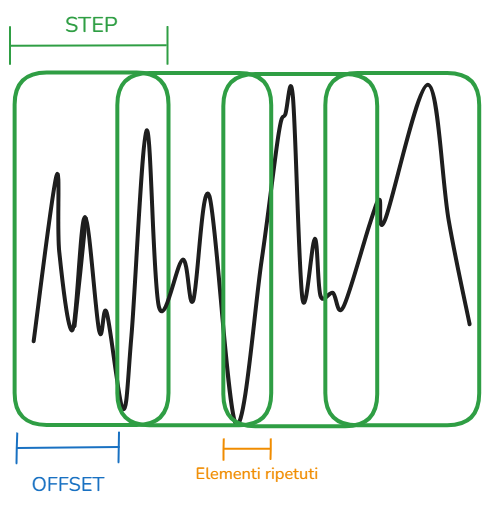
\includegraphics[width=0.5\linewidth]{images//Capitolo4/OFFSET_STEP.png}
    \caption{Finestre ROCKET su timeseries con OFFSET}
    \label{fig:OFFSET_STEP}
\end{figure}

\subsection{Metriche Rilevate}
In questo paragrafo riportiamo le metriche riscontrate dell'esecuzione di ROCKET e ROCKAD con diversi valori di: numero di kernel, valore di OFFSET e numero di n\textunderscore neighbors.

Le metriche, data la conformazione del dataset, sono divise per canale, questo porta ad una scelta che bisogna effettuare, ossia come calcolare le metriche.
Per uniformare i valori delle metriche, in particolare dell'F1, scegliamo di conservare in un file \textit{.json} tutti i valori necessari (TP, TN, FP, FN) per calcolare le metriche dopo l'analisi di tutti i channel, ritardando così il calcolo.
Riportiamo queste metriche nella Tabella \ref{tab:NASA_Posticipato}.
Un'altra possibile soluzione prevede di calcolare subito le metriche di ogni canale e poi fare la media alla fine di tutte le metriche, questo calcolo è meno accurato e tende a produrre metriche minori, riportiamo comunque i risultati ottenuti nella Tabella \ref{tab:NASA_Media}.

\begin{table}[!ht]
    \centering % Correttamente posizionato
    \begin{adjustbox}{max width=\textwidth}
        \begin{tabular}{|c|c|c|c|c|c|c|c|}
        \hline
        \textbf{Accuracy} &\textbf{Precision}  & \textbf{Recall} & \textbf{F1} & \textbf{MCC} & \textbf{AUC-PR} & \textbf{AUC-ROC} & \textbf{NScore}\\
        \hline
        \multicolumn{8}{|c|}{\textbf{ROCKET}} \\
        \hline
        \multicolumn{8}{|c|}{kernel=10.000, n\textunderscore neighbors=1 e OFFSET=50} \\
        \hline
         \textbf{0.735} & \textbf{0.299} & 0.471 &0.366  & \textbf{0.232 }& 0.286& 0.652 & 0.378 \\
        \hline
        \multicolumn{8}{|c|}{kernel=10.000, n\textunderscore neighbors=2 e OFFSET=30} \\
        \hline
         0.719 & 0.284 & \textbf{0.482} &0.357  & 0.219 & 0.28& 0.647 & 0.371 \\
        \hline
        \multicolumn{8}{|c|}{kernel=1000, n\textunderscore neighbors=1 e OFFSET=50} \\
        \hline
         0.731 & 0.296 & 0.478 &\textbf{0.367}  & 0.231 & \textbf{0.288}& \textbf{0.654} & \textbf{0.384} \\
        \hline
        \multicolumn{8}{|c|}{kernel=1000, n\textunderscore neighbors=2 e OFFSET=30} \\
        % da cambiare
        \hline
         0.721 & 0.284 & 0.473 &0.355  & 0.217 & 0.281& 0.647 & 0.37 \\
        \hline
        \multicolumn{8}{|c|}{kernel=1000, n\textunderscore neighbors=5 e OFFSET=10} \\
        % da cambiare
        \hline
         0.730 & 0.295 & 0.477 &0.365  & 0.230 & 0.278& 0.648 & 0.382 \\
         \hline
        \multicolumn{8}{|c|}{\textbf{ROCKAD}} \\
        \hline
        \multicolumn{8}{|c|}{kernel=10.000, n\textunderscore neighbors=1 e OFFSET=50} \\
        \hline
        \textbf{0.593} & 0.106 & 0.19 &0.136  & -0.129 &0.287 &\textbf{0.651}  &0.378 \\
        \hline
        \multicolumn{8}{|c|}{kernel=10.000, n\textunderscore neighbors=2 e OFFSET=30} \\
        \hline
        0.628 & \textbf{0.131} & 0.207 &0.16  & \textbf{-0.076} &\textbf{0.29} &0.646  &0.379 \\
        \hline
        \multicolumn{8}{|c|}{kernel=1000, n\textunderscore neighbors=2 e OFFSET=50} \\
        \hline
        0.6 & 0.106 & 0.193 &0.137  & -0.131 &0.286 &\textbf{0.651}  &0.378 \\
        \hline
        \multicolumn{8}{|c|}{ROCKAD con 1000 kernel, n\textunderscore neighbors=2 e OFFSET=30} \\
        \hline
        0.614 & 0.129 & \textbf{0.218} &\textbf{0.162}  & -0.083 &\textbf{0.29} &0.646  &\textbf{0.381} \\
        \hline
        \multicolumn{8}{|c|}{kernel=1000, n\textunderscore neighbors=5 e OFFSET=10} \\
        % da cambiare
        \hline
         0.453 & 0.093 & 0.25 &0.136  & 0.26 & 0.292& 0.65 & \textbf{0.381 }\\
        \hline
        \end{tabular}
    \end{adjustbox}
    \caption{Calcolo delle metriche globali (con la somma TP, TF, FP, FN)}
    \label{tab:NASA_Posticipato}
\end{table}
\begin{table}[!ht]
    \centering
    \begin{adjustbox}{max width=\textwidth}
        \begin{tabular}{|c|c|c|c|c|c|c|c|}
        \hline
        \textbf{Accuracy} &\textbf{Precision}  & \textbf{Recall} & \textbf{F1} & \textbf{MCC} & \textbf{AUC-PR} & \textbf{AUC-ROC} & \textbf{NScore}\\
        \hline
        \multicolumn{8}{|c|}{\textbf{ROCKET}} \\
        \hline
        \multicolumn{8}{|c|}{kernel=10.000, n\textunderscore neighbors=1 e OFFSET=50} \\
        \hline
        \textbf{0.723} & \textbf{0.357} & 0.499 &0.328  & 0.0 &0.736 & 0.514 & 0.0\\
        \hline
        \multicolumn{8}{|c|}{kernel=10.000, n\textunderscore neighbors=2 e OFFSET=30} \\
        \hline
        0.709 & 0.341 & \textbf{0.519} &\textbf{0.337}  & 0.0 &0.736 & \textbf{0.517} & 0.0\\
        \hline
        \multicolumn{8}{|c|}{kernel=1000, n\textunderscore neighbors=1 e OFFSET=50} \\
        \hline
        0.722 & 0.354 & 0.501 &0.320  & 0.0 &0.738 & 0.510 & 0.0\\
        \hline
        \multicolumn{8}{|c|}{kernel=1000, n\textunderscore neighbors=2 e OFFSET=30} \\
        % da cambiare
        \hline
        0.712 & 0.327 & 0.499 &0.319  & 0.0 &0.737 & 0.509 & 0.0\\
        \hline
        \multicolumn{8}{|c|}{kernel=1000, n\textunderscore neighbors=5 e OFFSET=10} \\
        % da cambiare
        \hline
        0.719 & 0.355 & 0.504 &0.332  & 0.0 &\textbf{0.741} & 0.505 & 0.0\\
        \hline
        \multicolumn{8}{|c|}{\textbf{ROCKAD}} \\
        \hline
        \multicolumn{8}{|c|}{ROCKAD con 10.000, n\textunderscore neighbors=2 e OFFSET=50} \\
        \hline
        0.593 & 0.119 & 0.167 &0.09  & -0.111 & \textbf{0.729}& \textbf{0.516} & 0.454\\
        \hline
        \multicolumn{8}{|c|}{kernel=10.000, n\textunderscore neighbors=2 e OFFSET=30} \\
        \hline
        \textbf{0.622} & 0.114 & 0.191 &0.108  & -0.079 & 0.728& 0.514 & \textbf{0.473}\\
        \hline
        \multicolumn{8}{|c|}{ROCKAD con 1000 kernel, n\textunderscore neighbors=2 e OFFSET=50} \\
        \hline
        0.594 & 0.107 & 0.16 &0.088  & -0.109 & 0.725& 0.510 & 0.455\\
        \hline
        \multicolumn{8}{|c|}{kernel=1000, n\textunderscore neighbors=2 e OFFSET=30} \\
        \hline
        0.612 & \textbf{0.128} & 0.192 &0.115  & -0.09 & 0.723& 0.503 & 0.448\\
        \hline
        \multicolumn{8}{|c|}{kernel=1000, n\textunderscore neighbors=5 e OFFSET=10} \\
        % da cambiare
        \hline
        0.476 & 0.127 & \textbf{0.291} &\textbf{0.14}  & \textbf{0.136} &0.728 & 0.499 & 0.467\\
        \hline
        \end{tabular}
    \end{adjustbox}
    \caption{Metriche calcolate con la media}
    \label{tab:NASA_Media}
\end{table}
\pagebreak

Per avere un valutazione più approfondita abbiamo effettuato test anche con altri classificatori, oltre a NearestNeighborOCC.
Abbiamo preso in considerazione tre algoritmi, presenti all'interno della librerie fornite da \texttt{scikit-learn}$^{\text{\cite{scikit-learn}}}$, questi sono:
\begin{itemize}
    \item OneClassSVM: sfrutta SVM, un algoritmo di tipo supervisionato che cerca di massimizzare il margine tra le classi, per delineare una frontiera che divide i valori anomali da quelli normali;
    \item Isolation Forest: sceglie una caratteristica casualmente e, tramite quella, isola le osservazioni in base ad una soglia, sempre scelta casualmente nell'intervallo di valori della caratteristica; questo processo avviene in modo ricorsivo, portando ad evidenziare le anomalie come i percorsi più brevi;
    \item Local Outlier Factor (LOF): si basa sul calcolo di un punteggio di anomalia per ogni osservazione, questo avviene tramite la misurazione della deviazione della densità locale rispetto ad i nodi vicini.
\end{itemize}

Le metriche riportate nella tabella sono calcolate dopo aver effettuato la somma di tutti i valori di TP, TN, FP e FN, così da uniformare la valutazione.
La colonna parametri che troviamo nella Tabella \ref{tab:ROCKAD_NASA_AlgoritmiVari-ROCKET} e nella Tabella \ref{tab:ROCKAD_NASA_AlgoritmiVari_ROCKAD} corrispondono ripetitivamente a (numero di kernel, OFFSET) e (numero di kernel, n\textunderscore neighbors, OFFSET).
\begin{table}[!ht]
    \centering
    \begin{adjustbox}{max width=\textwidth}
    \begin{tabular}{|c|c|c|c|c|c|c|c|c|}
    \hline
         \textbf{Parametri} & \textbf{Accuracy} &\textbf{Precision}  & \textbf{Recall} & \textbf{F1} & \textbf{MCC} & \textbf{AUC-PR} & \textbf{AUC-ROC} & \textbf{N-Scores}\\
        \hline
        \multicolumn{9}{|c|}{\textbf{OneClassSVM}} \\
        \hline
         (10.000, 250)&\textbf{0.748}& \textbf{0.167}& 0.148& \textbf{0.157}&\textbf{0.009}&\textbf{ 0.166} &\textbf{0.356} & \textbf{0.167}\\
         \hline
         (10.000, 150)&0.66& 0.109& 0.152& 0.127&-0.088& 0.165 &0.341 & 0.149\\
         \hline
         (1000, 50) &0.526& 0.079& 0.181& 0.11&-0.218& 0.164 &0.334 & 0.122\\
         \hline
        (1000, 10)&0.5 &0.083 &\textbf{0.205} &0.118 & -0.23& 0.161& 0.324&0.12\\
         \hline
         \multicolumn{9}{|c|}{\textbf{Isolation Forest}} \\
         \hline
         (10.000, 50)&0.271& 0.124& 0.575& 0.204&-0.321& \textbf{0.129} &0.379 & 0.093\\
         \hline
         (1000, 50) &\textbf{0.285}& \textbf{0.125}& 0.568& \textbf{0.205}&\textbf{-0.291}&\textbf{ 0.129} &\textbf{0.38} & \textbf{0.116}\\
         \hline
         (1000, 10)&0.211 &0.120 &\textbf{0.611} &0.201 & -0.492& 0.125& 0.365&0.096\\
         \hline
         \multicolumn{9}{|c|}{\textbf{Local Outlier Factor}} \\
         \hline
         (10.000, 50)&0.19 &0.14 &0.773 &0.237 &-0.384 &\textbf{0.139} &\textbf{0.406}& \textbf{0.15}\\
         \hline
         (1000, 50)&0.19 &0.14 &0.773 &0.237 & -0.383 &0.137 &0.404& 0.132\\
         \hline
         (1000, 10)&\textbf{0.194} &\textbf{0.143} &\textbf{0.793} &\textbf{0.242} &\textbf{-0.331} &0.127 &0.364& 0.136\\
         \hline
    \end{tabular}
    \end{adjustbox}
    \caption{Test con classificatori diversi - ROCKET}
    \label{tab:ROCKAD_NASA_AlgoritmiVari-ROCKET}
\end{table}

\begin{table}[!ht]
    \centering
    \begin{adjustbox}{max width=\textwidth}
    \begin{tabular}{|c|c|c|c|c|c|c|c|c|}
    \hline
         \textbf{Parametri} & \textbf{Accuracy} &\textbf{Precision}  & \textbf{Recall} & \textbf{F1} & \textbf{MCC} & \textbf{AUC-PR} & \textbf{AUC-ROC} & \textbf{N-Scores}\\
        \hline
        \multicolumn{9}{|c|}{\textbf{OneClassSVM}} \\
        \hline
         (10.000, 2, 50)&\textbf{0.726}& 0.09& 0.069& 0.078&-0.086& 0.287 &\textbf{0.651} & 0.378\\
         \hline
         (1000, 2, 50) &0.722& 0.09& \textbf{0.72}& 0.08&-0.087& 0.286 &\textbf{0.651} & 0.378\\
         \hline
        (1000, 5, 10)&0.654 &\textbf{0.141} &0.201 &\textbf{0.166} & \textbf{-0.05}& \textbf{0.292}& 0.65&\textbf{0.381}\\
         \hline
         \multicolumn{9}{|c|}{\textbf{Isolation Forest}} \\
         \hline
         (10.000, 2, 50)&\textbf{0.706}& 0.092& 0.084& 0.088&\textbf{-0.094}& 0.287 &\textbf{0.651} & 0.378\\
         \hline
         (1000, 2, 50) &0.701& 0.094& 0.89& 0.091&\textbf{-0.094}& 0.286 &\textbf{0.651} & 0.378\\
         \hline
         (1000, 5, 10)&0.6 &\textbf{0.113} &\textbf{0.196} &\textbf{0.144} & -0.117& \textbf{0.292}& 0.65&\textbf{0.381}\\
         \hline
         \multicolumn{9}{|c|}{\textbf{Local Outlier Factor}} \\
         \hline
         (10.000, 2, 50)&0.203 &0.150 &0.803 &0.253 &-0.29 &0.287 &\textbf{0.651}& 0.378\\
         \hline
         (1000, 2, 50)&0.201 &0.150 &0.799 &0.252 & -0.303 &0.286 &\textbf{0.651}& 0.378\\
         \hline
         (1000, 5, 10)&\textbf{0.206} &\textbf{0.155} &\textbf{0.82} &\textbf{0.261} &\textbf{-0.256} &\textbf{0.292} &0.65& \textbf{0.381}\\
         \hline
    \end{tabular}
    \end{adjustbox}
    \caption{Test con classificatori diversi - ROCKAD}
    \label{tab:ROCKAD_NASA_AlgoritmiVari_ROCKAD}
\end{table}

% da aggiungere alemeno una prova con 20.000 kernel ed una con 1000 ossia quello di default
\pagebreak

\subsection{Panoramica su OPS\textunderscore SAT con Algoritmi}
In questa sezione riportiamo i risultati dei test effettuati su OPS\textunderscore SAT, con i modelli appena testati su NASA.
Questo ci permette di avere una visione di insieme del comportamento di questi modelli, in relazione anche al dataset utilizzato.
Tutti i test sono effettuati utilizzando i migliori parametri riscontrati per ROCKAD, ossia 10 estimatori e 10.000 kernel, come possiamo vedere nella Tabella \ref{tab:ROCKAD_OPS-SAT}; per ROCKET invece non abbiamo molti parametri da modificare, ma manteniamo il numero di kernel di default pari a 10.000.
\begin{table}[h!]
    \centering % Correttamente posizionato
    \begin{adjustbox}{max width=\textwidth}
        \begin{tabular}{|c|c|c|c|c|c|c|c|c|}
        \hline
        \textbf{Algoritmo} & \textbf{Accuracy} &\textbf{Precision}  & \textbf{Recall} & \textbf{F1} & \textbf{MCC} & \textbf{AUC-PR} & \textbf{AUC-ROC} & \textbf{N-Scores}\\
        \hline
        \multicolumn{9}{|c|}{\textbf{ROCKET}} \\
        \hline
         \textbf{OneClassSVM} & 0.192 & 0.126 & 0.134 &0.13  & -0.1 & \textbf{0.463}& \textbf{0.392}& \textbf{0.371}\\
        \hline
        \textbf{Isolation Forest} & 0.385 & 0.144 & 0.269 &0.187  & -0.132 & 0.442& 0.336&0.339 \\
        \hline
        \textbf{Local Outlier Factor} & \textbf{0.4} & \textbf{0.148} &\textbf{ 0.28} &\textbf{0.194}  & \textbf{-0.098} & 0.441& 0.334&\textbf{0.371} \\
        \hline
        \multicolumn{9}{|c|}{\textbf{ROCKAD}} \\
        \hline
         \textbf{OneClassSVM} & 0.3 & \textbf{0.3} & 0.3 &0.3  & -0.4 & 0.757& 0.704 &0.677\\
        \hline
        \textbf{Isolation Forest} & 0.277 & 0.234 & 0.287 &0.247  & -0.476 & 0.757& 0.704&0.677 \\
        \hline
        \textbf{Local Outlier Factor} & \textbf{0.408} & 0.295 & \textbf{0.426} &\textbf{0.31}  & \textbf{-0.246} & 0.757& 0.704&0.677\\
        \hline
        \end{tabular}
    \end{adjustbox}
    \caption{Algoritmi diversi a confronto, ROCKET e ROCKAD su OPS\textunderscore SAT}
    \label{tab:AlgoritmiVari_OPS_SAT}
\end{table}



\subsection{Analisi dei risultati NASA e Problematiche dei Modelli}
Nel paragrafo successivo andremo ad analizzare i risultati elencati in tabella discutendo le migliori soluzioni.

La metrica più significativa tra tutte quelle calcolate, nel contesto del dataset NASA, è sicuramente il valore di \textit{F1 Score}.
Considerando quindi come metrica principale questa e il tempo impiegato per l'esecuzione, oltre a tutte le metriche secondarie riportate in tabella, possiamo osservare che nel caso di ROCKET i miglior valori dei parametri testati sono due:
\begin{itemize}
    \item  kernel=1000, n\textunderscore neighbors=1 e OFFSET=50: questi valori garantiscono metriche buone ed una velocità di esecuzione molto elevata, data la semplicità del KNN e dell'OFFSET abbastanza alto, portando ad una scarsa espressività e performance peggiori con dataset rumorosi. Nel nostro caso però potrebbe tornare utile per la velocità di esecuzione, che con un processore non troppo potente è un parametro importante;
    \item  kernel=10.000, n\textunderscore neighbors=1 e OFFSET=50: in questa soluzione utilizziamo il valore standard dei kernel lasciando invariati, rispetto al modello sopra, gli altri valori. Un maggior numero di kernel porta ad un maggior numero di caratteristiche e quindi di informazioni per le classificazioni, che però sono semplificate dalla semplicità del KNN e dell'OFFSET. Il problema principale di questi parametri è il tempo di esecuzione prolungato ma non in modo eccessivo;
    \item kernel=1000, n\textunderscore neighbors=5 e OFFSET=10: anche in questo caso le metriche sono comparabili al precedente, ma la velocità di esecuzione qui aumenta notevolmente, insieme ad un aumento dell'espressività del KNN e dal numero basso di OFFSET che rende l'algoritmo più robusto e stabile.
\end{itemize}

Per quanto riguarda ROCKAD, avremo anche qui due possibili soluzioni con metriche simili: la prima con 10.000 kernel, n\textunderscore neighbors=2 e OFFSET=30; la seconda con 1000 kernel, n\textunderscore neighbors=2 e OFFSET=30.
Rispetto a ROCKET però, il tempo di esecuzione cambia in modo ancora più marcato, portando all'esclusione della prima soluzione, che utilizza il numero di kernel standard per ROCKET (10.000).
\pagebreak
\subsection{Analisi Test con Classificatori Alternativi}
I test effettuati con algoritmi diversi, rispetto a quelli utilizzati nei paper o nelle analisi precedenti (KNN e NearestNeighborOCC), ci permettono di capire meglio se i modelli scelti in partenza per l'analisi e quelli di default di ROCKET e ROCKAD sono i migliori.
Questo porta alla ricerca di alternative più efficienti, tramite confronti e riflessioni.

I modelli alternativi sono stati scelti sulla base del dataset NASA, quindi sono tutti algoritmi unsupervised, questi permettono di superare il problema della lunghezza troppo breve delle timeseries per il KNN, che non aveva abbastanza nodi per la classificazione in alcuni canali.

Nel caso di ROCKET, gli algoritmi Isolation Forest, OneClassSVM e Local Outlier Factor si comportano male, avendo un F1 minore in tutti i casi, rispetto ai modelli standard, e comportandosi addirittura peggio di un classificatore casuale, come possiamo notare dal valore di MCC negativo (\ref{tab:ROCKAD_NASA_AlgoritmiVari-ROCKET}).

Confrontando comunque Local Outlier Factor (LOF), con il miglior risultato ottenuto con KNN, osserviamo che LOF ha un valore molto alto di recall, ossia permette di rilevare un maggior numero di anomalie, a discapito della precisione, che invece rimane molto bassa.
Questo rapporto ci permette di dire che LOF classifica molti falsi positivi, che nel nostro caso è una problematica fondamentale.

In generale quindi possiamo affermare che con ROCKET, il miglior algoritmo è KNN, dato che LOF ha metriche peggiori su tutti gli aspetti.

\begin{table}[h!]
    \centering
    \begin{adjustbox}{max width=\textwidth}
        \begin{tabular}{|c|c|c|c|c|c|c|c|c|}
        \hline
        \textbf{Modello} & \textbf{Accuracy} &\textbf{Precision}  & \textbf{Recall} & \textbf{F1} & \textbf{MCC} & \textbf{AUC-PR} & \textbf{AUC-ROC} & \textbf{NScore}\\
        \hline
        \textbf{LOF} & 0.194 & 0.143 & 0.793 &0.242  & -0.331 & 0.127 & 0.364 & 0.136 \\
        \hline
         \textbf{KNN} & 0.730 & 0.295 & 0.477 &0.365  & 0.230 & 0.278& 0.648 &0.382 \\
         \hline
        \end{tabular}
    \end{adjustbox}
    \caption{Confronto modelli con ROCKET}
    \label{tab:LOF_KNN}
\end{table}



Anche per ROCKAD, il miglior compromesso tra i diversi algoritmi rimane LOF, portando con se il problema dei troppi falsi positivi classificati.
A differenza però di ROCKET i risultati ottenuti da LOF qui sono più promettenti, infatti effettuando un confronto metrica per metrica tra LOF e NearestNeighborOCC, notiamo che Precision, Recall, AUC-ROC e F1 risultano superiori con il primo; questo indica una migliore capacità di classificare le anomalie pagando il prezzo, come detto in precedenza, di molti falsi positivi.
Con NearestNeighborOCC (NN\textunderscore OCC) invece, abbiamo valori maggiori delle metriche: Accuracy, MCC, AUC-PR e N-Score, che descrivono un modello che si comporta meglio di un algoritmo casuale e risulta più bilanciato.

La scelta tra i due modelli di classificazione dipende dall'utilizzo, LOF è sicuramente preferibile nel caso in cui volessimo trovare il maggior numero di anomalie, anche a costo di avere molti falsi positivi; invece come per il nostro caso, NearestNeighborOCC rappresenta una scelta più sicura e meno costosa in termini di controlli di falsi positivi.

\begin{table}[h!]
    \centering
    \begin{adjustbox}{max width=\textwidth}
        \begin{tabular}{|c|c|c|c|c|c|c|c|c|}
        \hline
        \textbf{Modello} & \textbf{Accuracy} &\textbf{Precision}  & \textbf{Recall} & \textbf{F1} & \textbf{MCC} & \textbf{AUC-PR} & \textbf{AUC-ROC} & \textbf{NScore}\\
        \hline
        \textbf{LOF} & 0.0.206 & 0.155& 0.82 &0.261  & -0.256 & 0.292 & 0.65 & 0.381 \\
        \hline
         \textbf{NN\textunderscore OCC} & 0.476 & 0.127 & 0.291 &0.14  & 0.136 & 0.728& 0.499 &0.467 \\
         \hline
        \end{tabular}
    \end{adjustbox}
    \caption{Confronto modelli con ROCKAD}
    \label{tab:LOF_NearestNeighborOCC}
\end{table}

\chapter{Risultati Empirici}
Dall'analisi dei valori notiamo che le migliori soluzioni escludono, per la maggior parte, l'utilizzo di 10.000 kernel se non con un valore di OFFSET abbastanza alto e di conseguenza un KNN molto semplificato.
Contrariamente a quanto affermato nei paper, relativi ad entrambi i modelli, ROCKET e ROCKAD non hanno un efficienza così elevata.
Prendendo, infatti, in considerazione il dataset OPS\textunderscore SAT, in caso di un valore basso di STEP, o nel caso del dataset NASA prendendo un valore basso di OFFSET, riscontriamo un efficienza non ottimale.

Nella fase di test, su OPS\textunderscore SAT, non è stato possibile estrarre le metriche con un valore di STEP inferiore a 250, dato che portava ad un esecuzione che avrebbe richiesto troppo tempo per terminare.

Per osservare meglio l'andamento dei modelli in base al numero di kernel, riportiamo le misurazioni rilevate dai test nei grafici in Figura \ref{fig:grafico_f1_ROCKET_OPS_SAT} e Figura \ref{fig:grafico_f1_ROCKAD_OPS_SAT}, che mettono in relazione il numero di kernel e la metrica F1.
\begin{figure}[!ht]
    \centering
    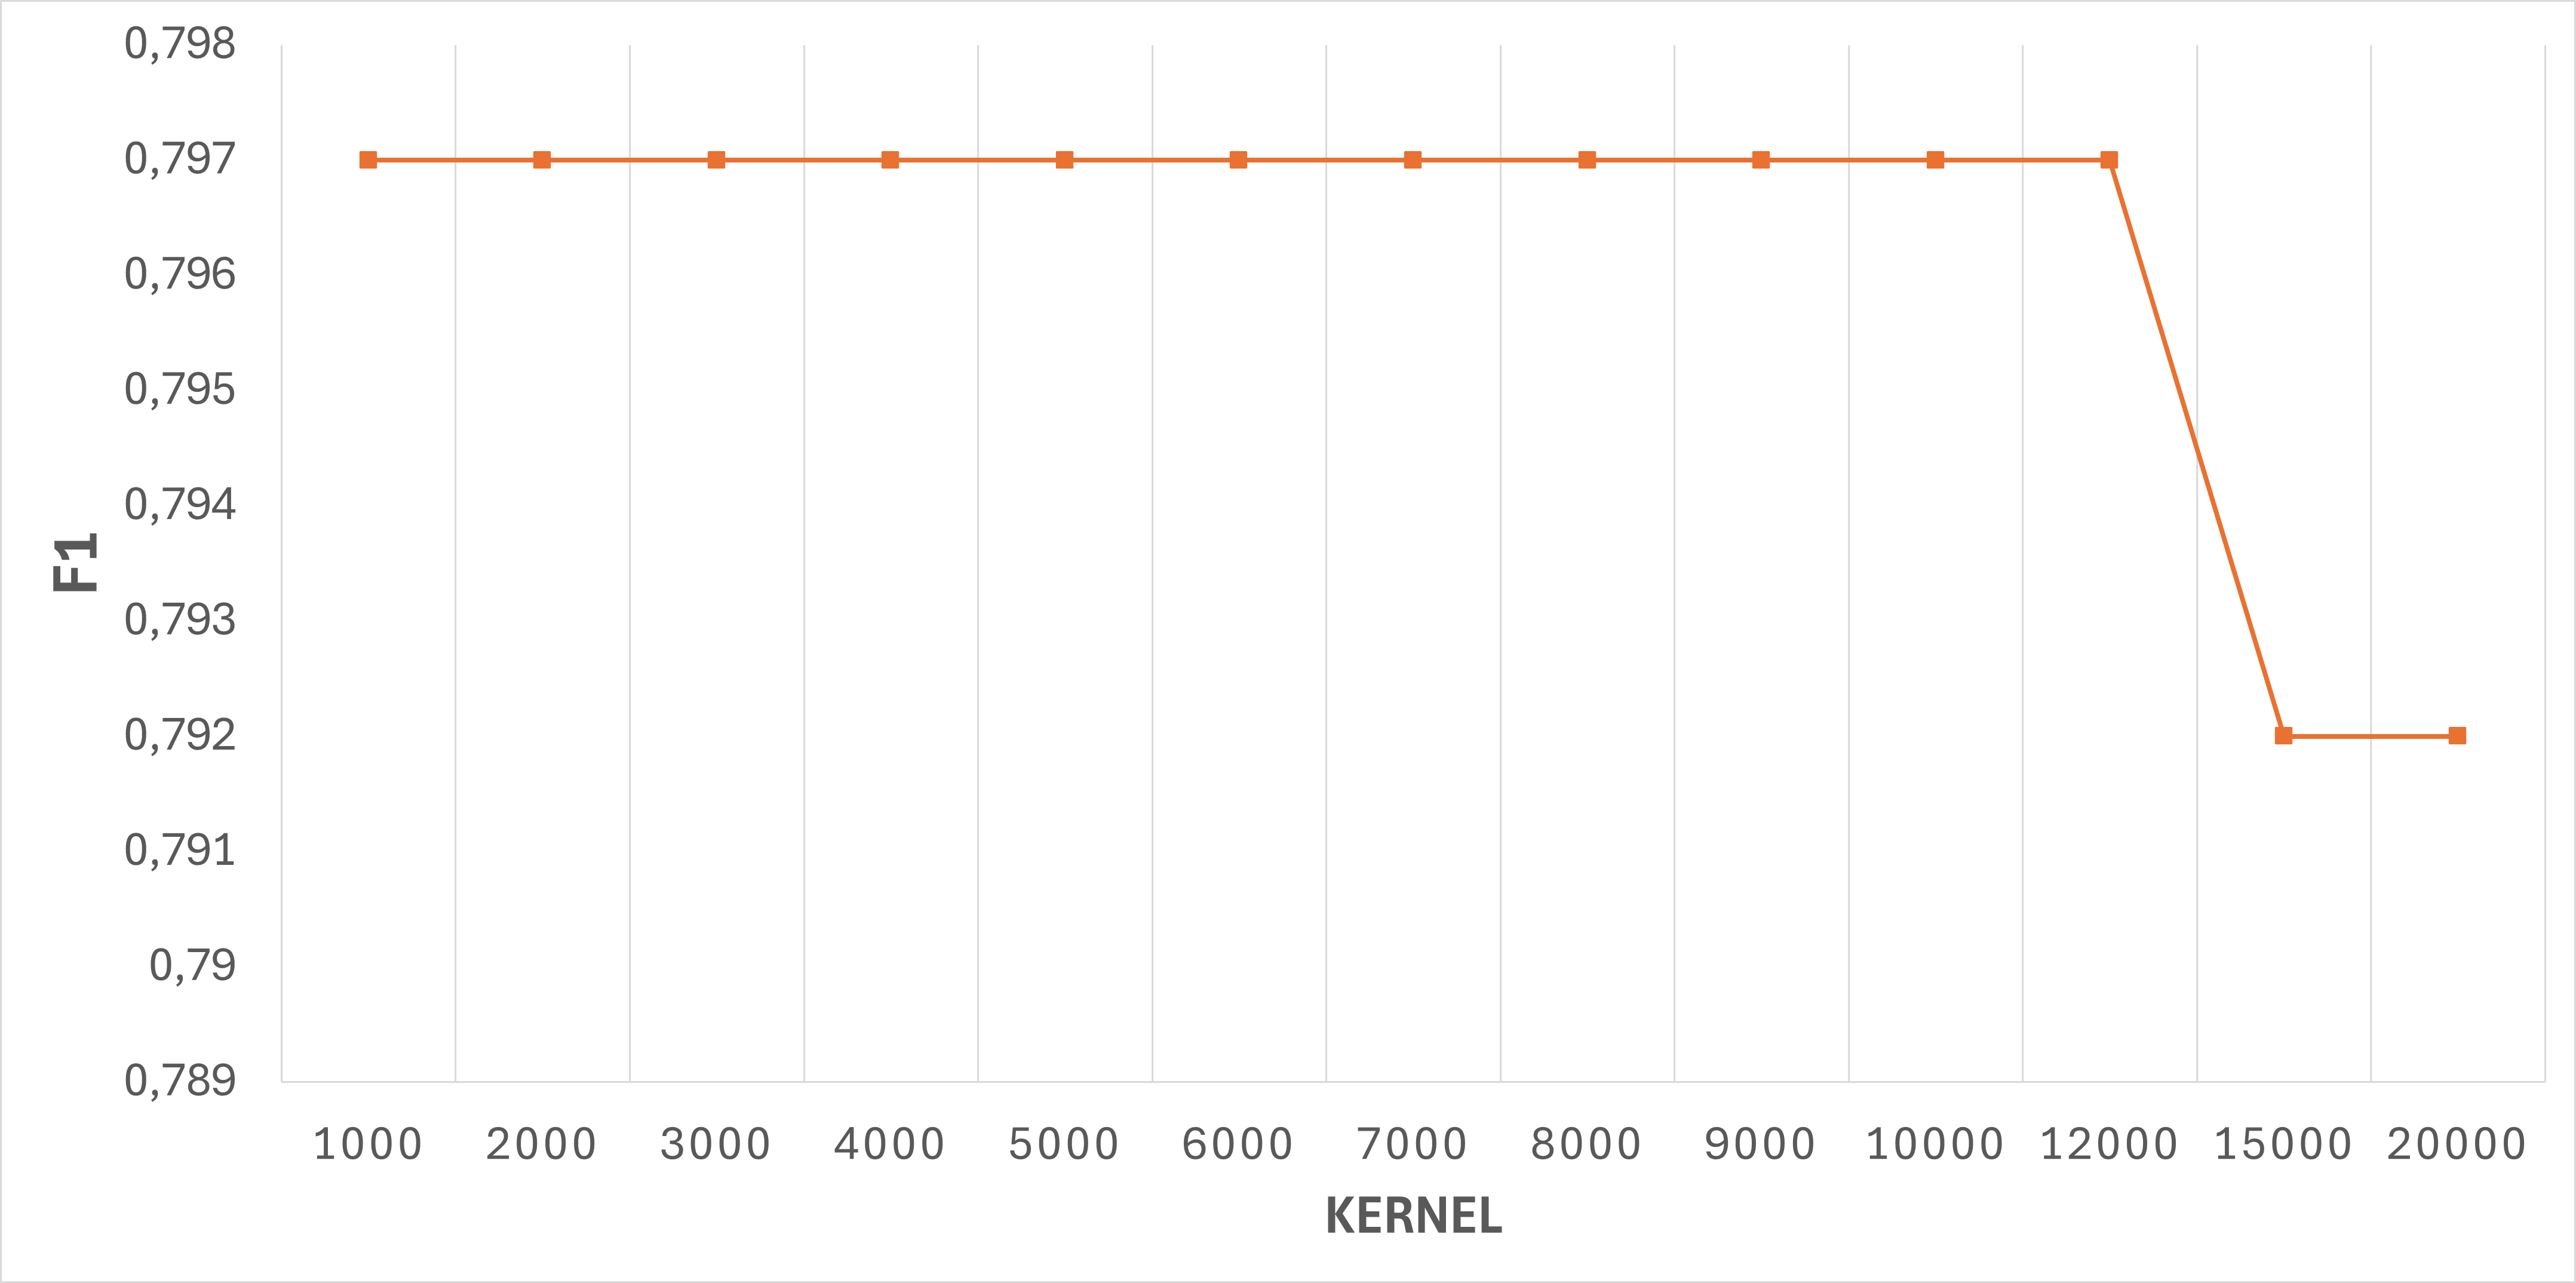
\includegraphics[width=0.9\linewidth]{images//Capitolo7/GraficoF1_ROCKET_OPS_SAT.png}
    \caption{Relazione tra F1 e Numero di Kernel - ROCKET}
    \label{fig:grafico_f1_ROCKET_OPS_SAT}
\end{figure}
\pagebreak

\begin{figure}[!ht]
    \centering
    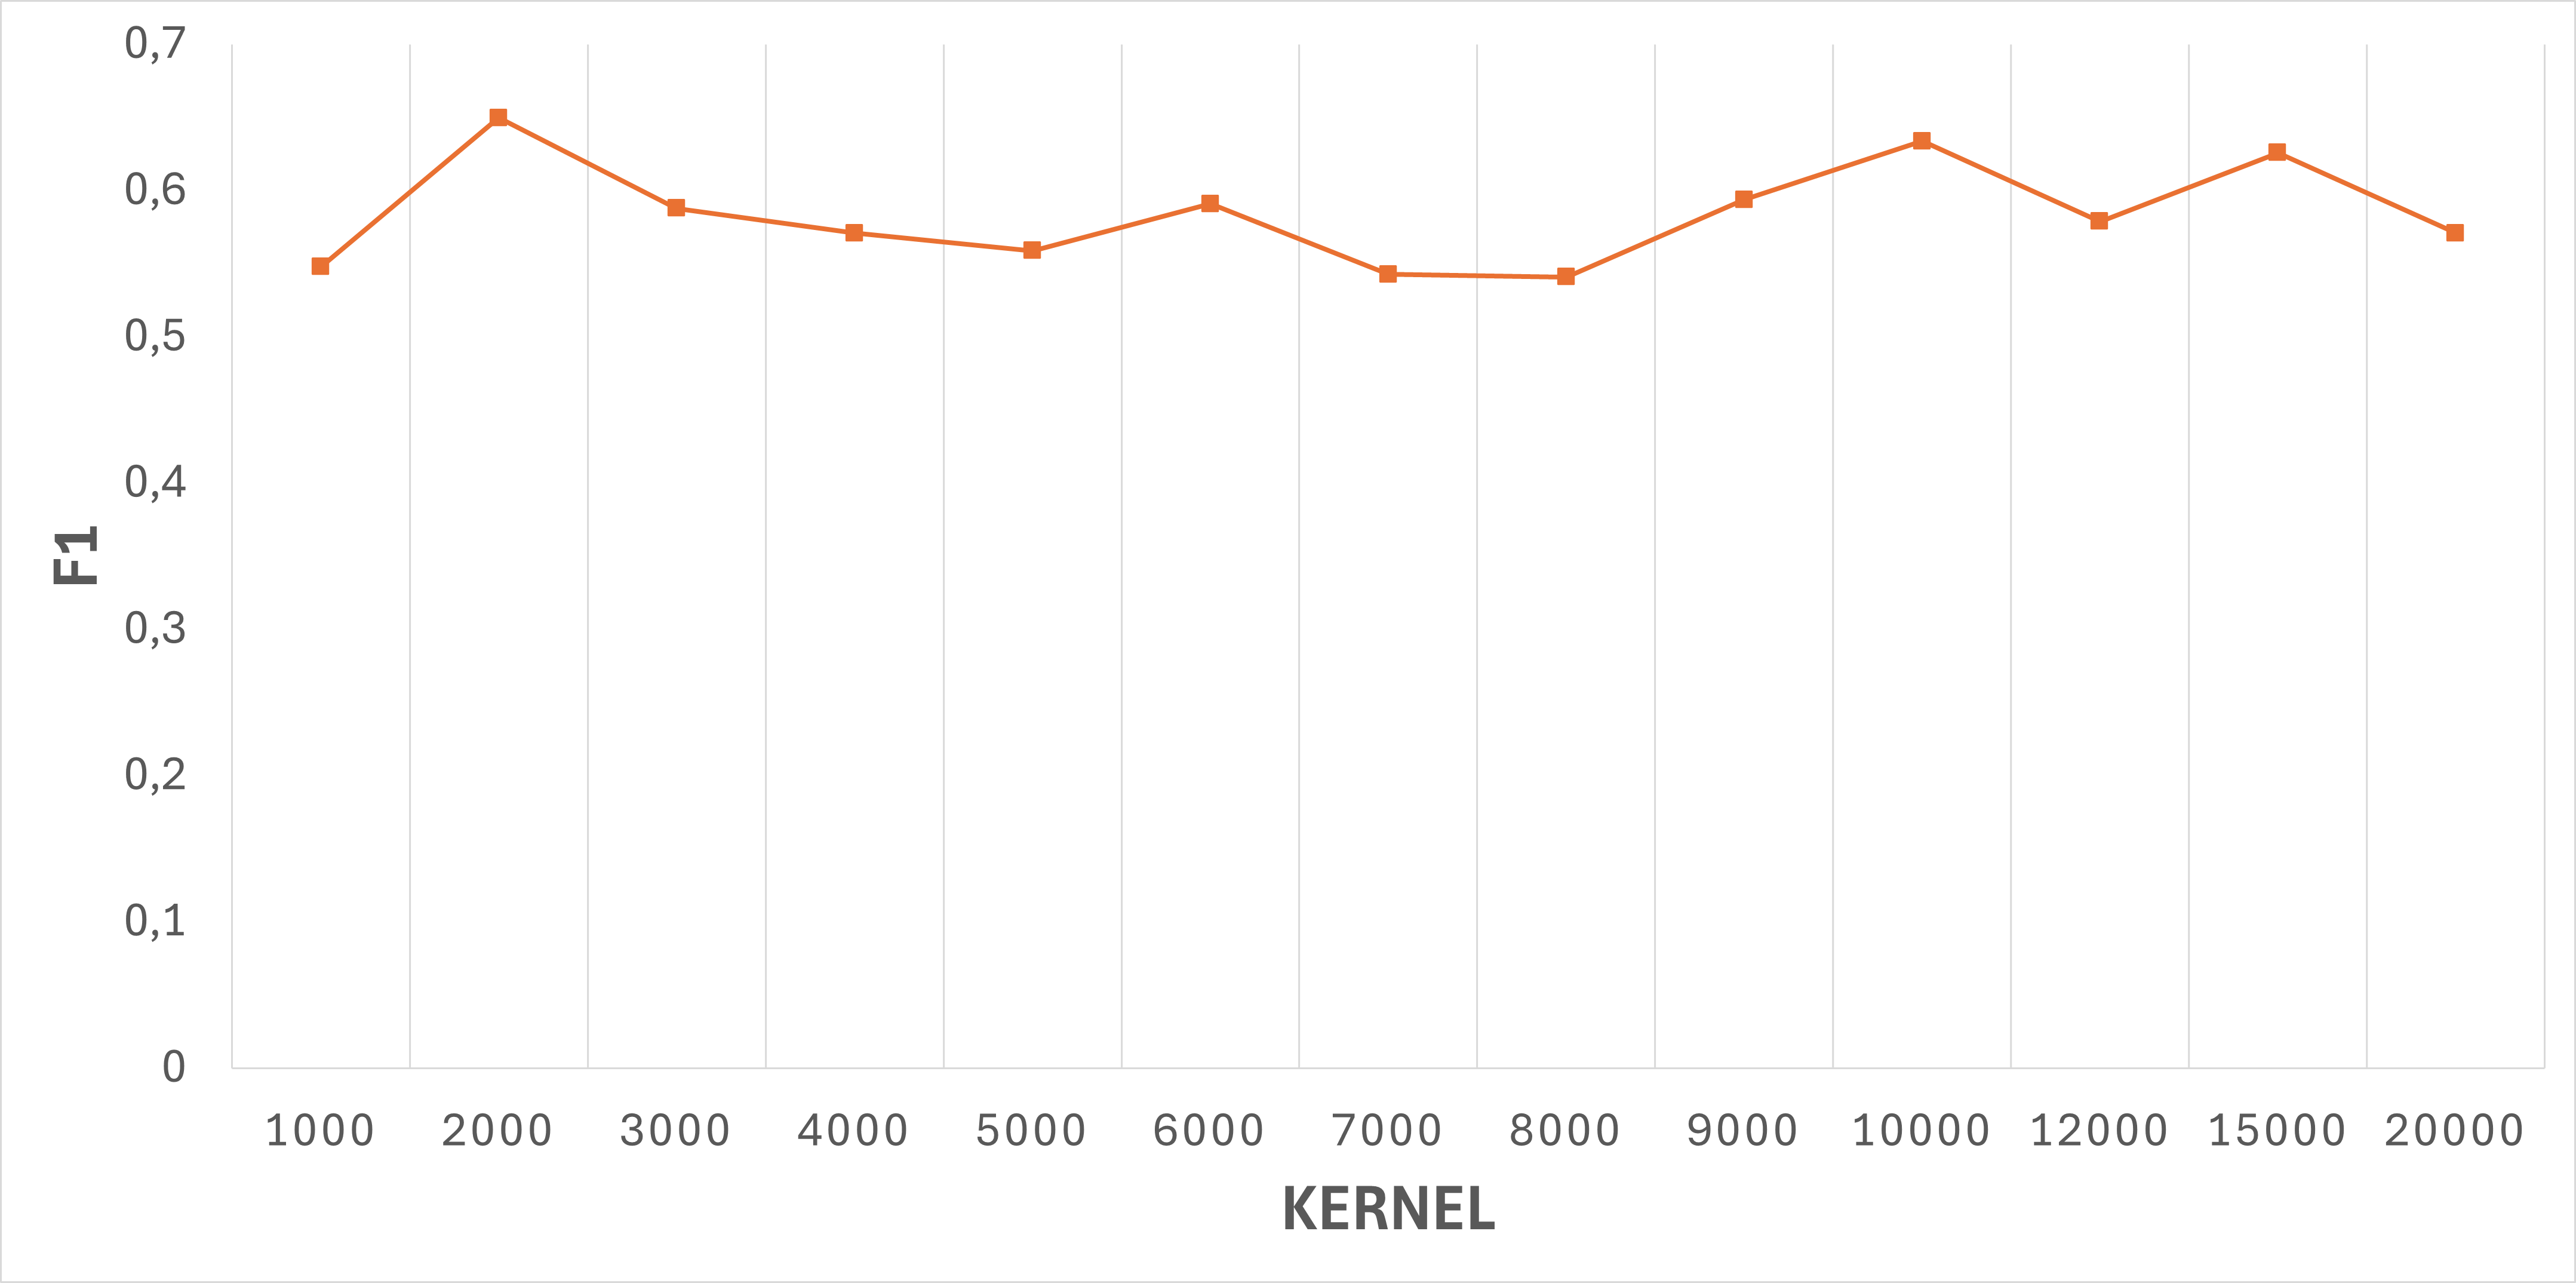
\includegraphics[width=0.9\linewidth]{images//Capitolo7/GraficoF1_ROCKAD_OPS_SAT.png}
    \caption{Relazione tra F1 e Numero di Kernel - ROCKAD}
    \label{fig:grafico_f1_ROCKAD_OPS_SAT}
\end{figure}

Oltre a tenere in considerazione l'F1, riportiamo in aggiunta, il tempo di esecuzione al variare del numero di kernel nel grafico in Figura \ref{fig:grafico_Tempo_ROCKET_OPS_SAT} per ROCKET e in quello in Figura \ref{fig:grafico_Tempo_ROCKAD_OPS_SAT} per ROCKAD.


\begin{figure}[!ht]
    \centering
    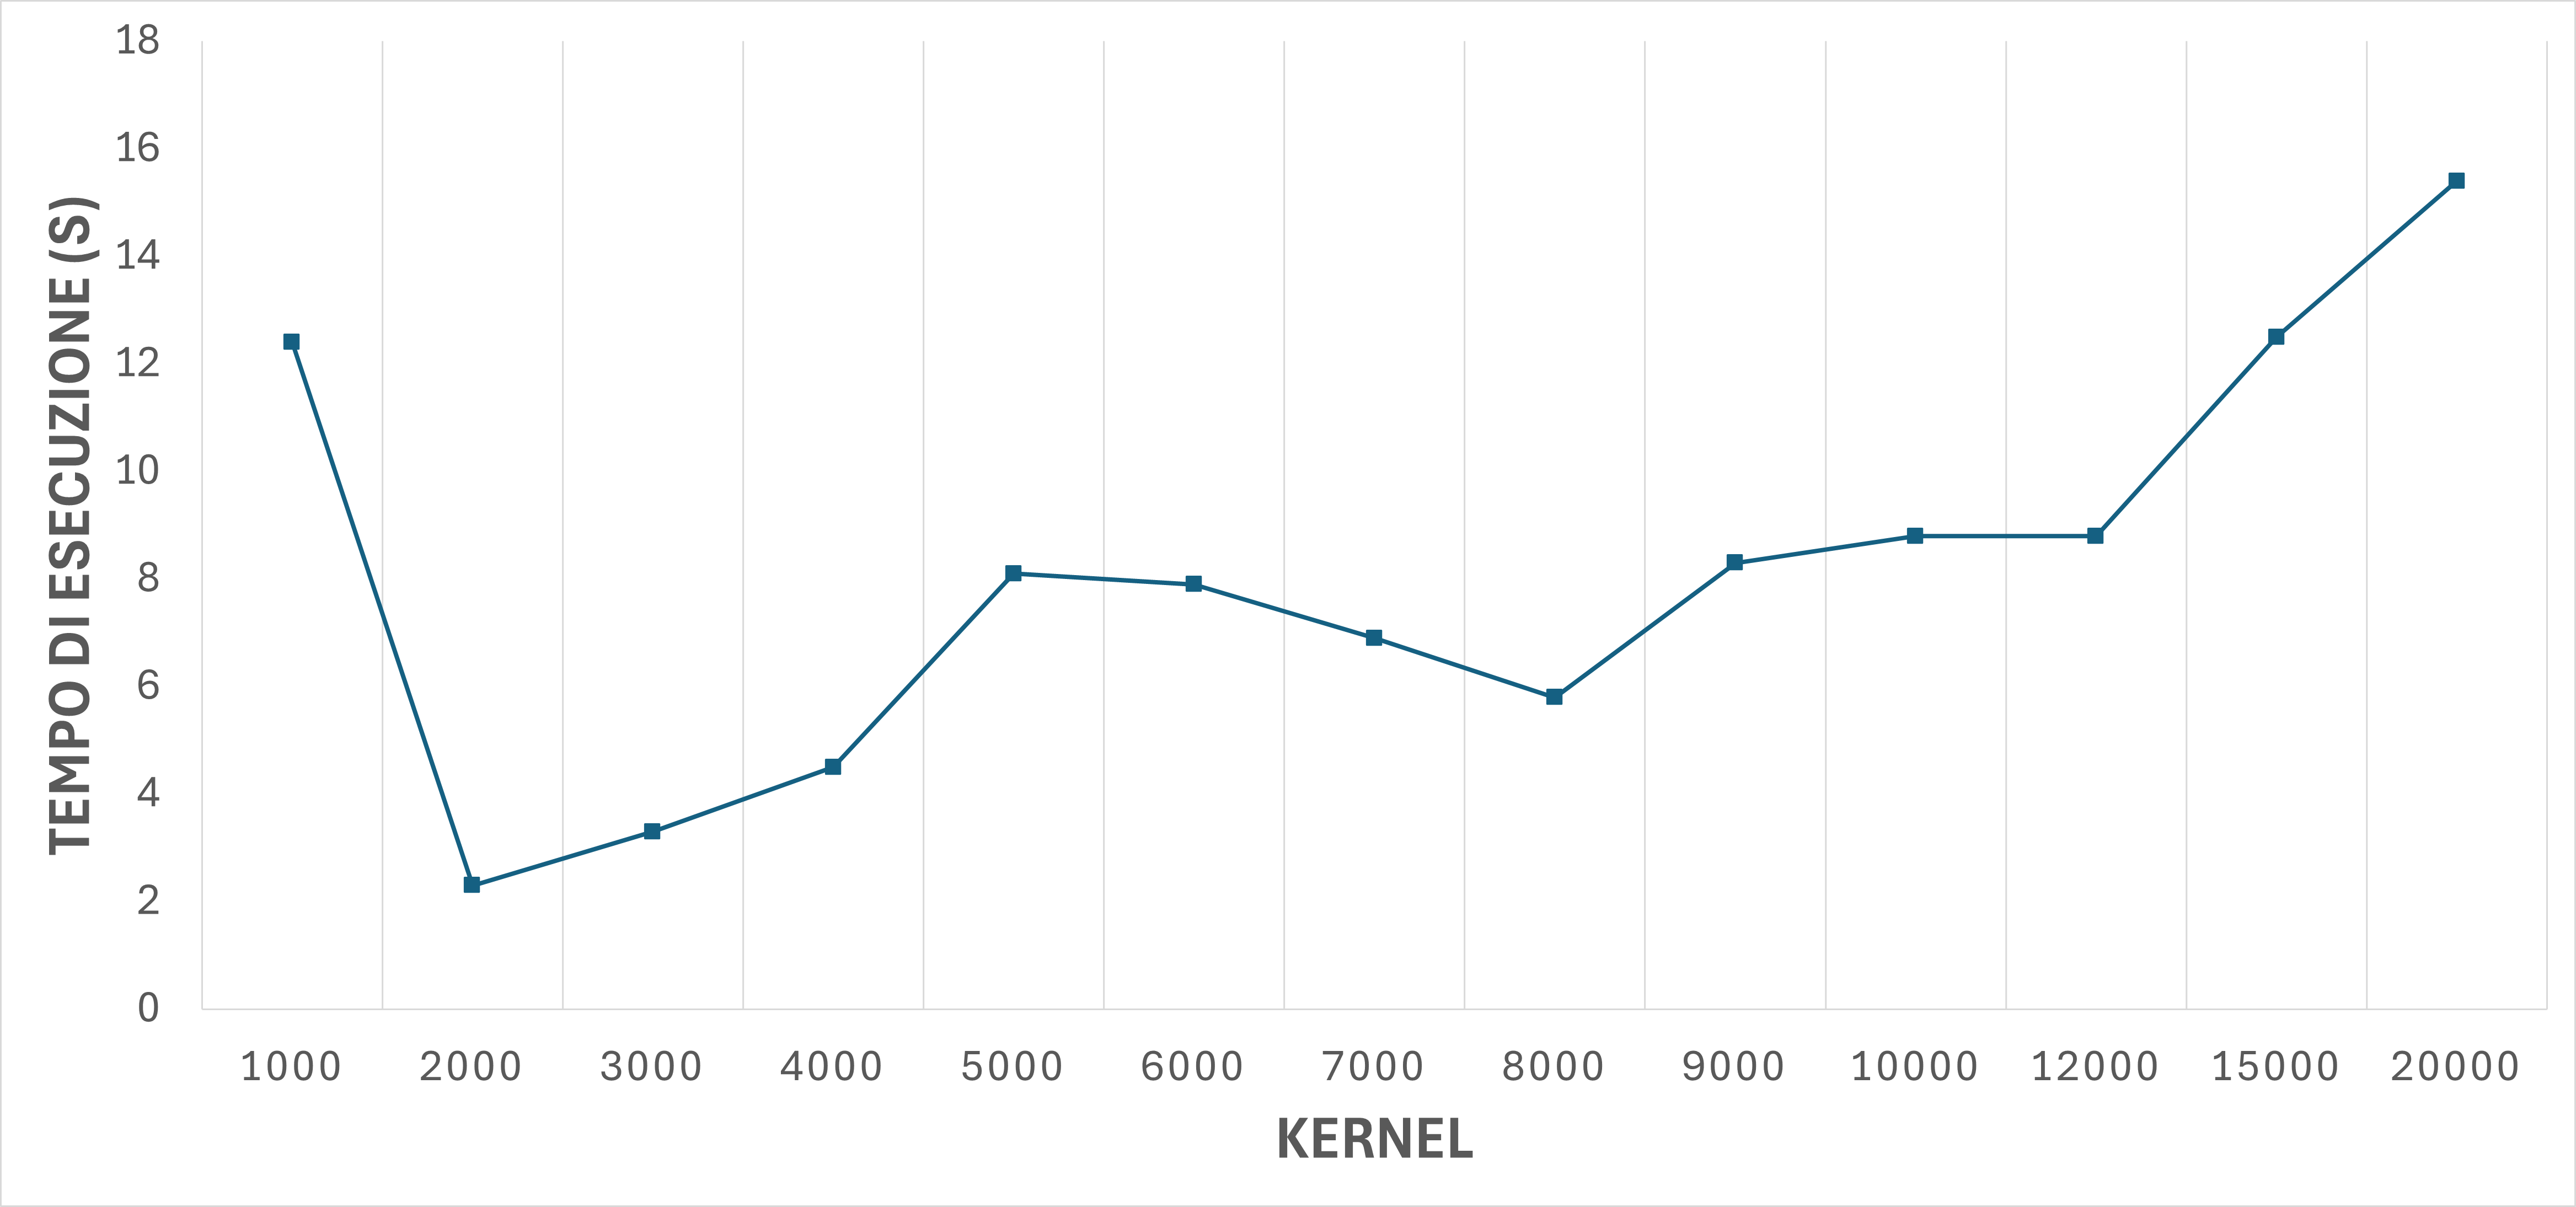
\includegraphics[width=0.9\linewidth]{images//Capitolo7/GraficoTempoEsecuzione_ROCKET_OPS_SAT.png}
    \caption{Relazione tra F1 e Numero di Kernel - ROCKET}
    \label{fig:grafico_Tempo_ROCKET_OPS_SAT}
\end{figure}

\begin{figure}[!ht]
    \centering
    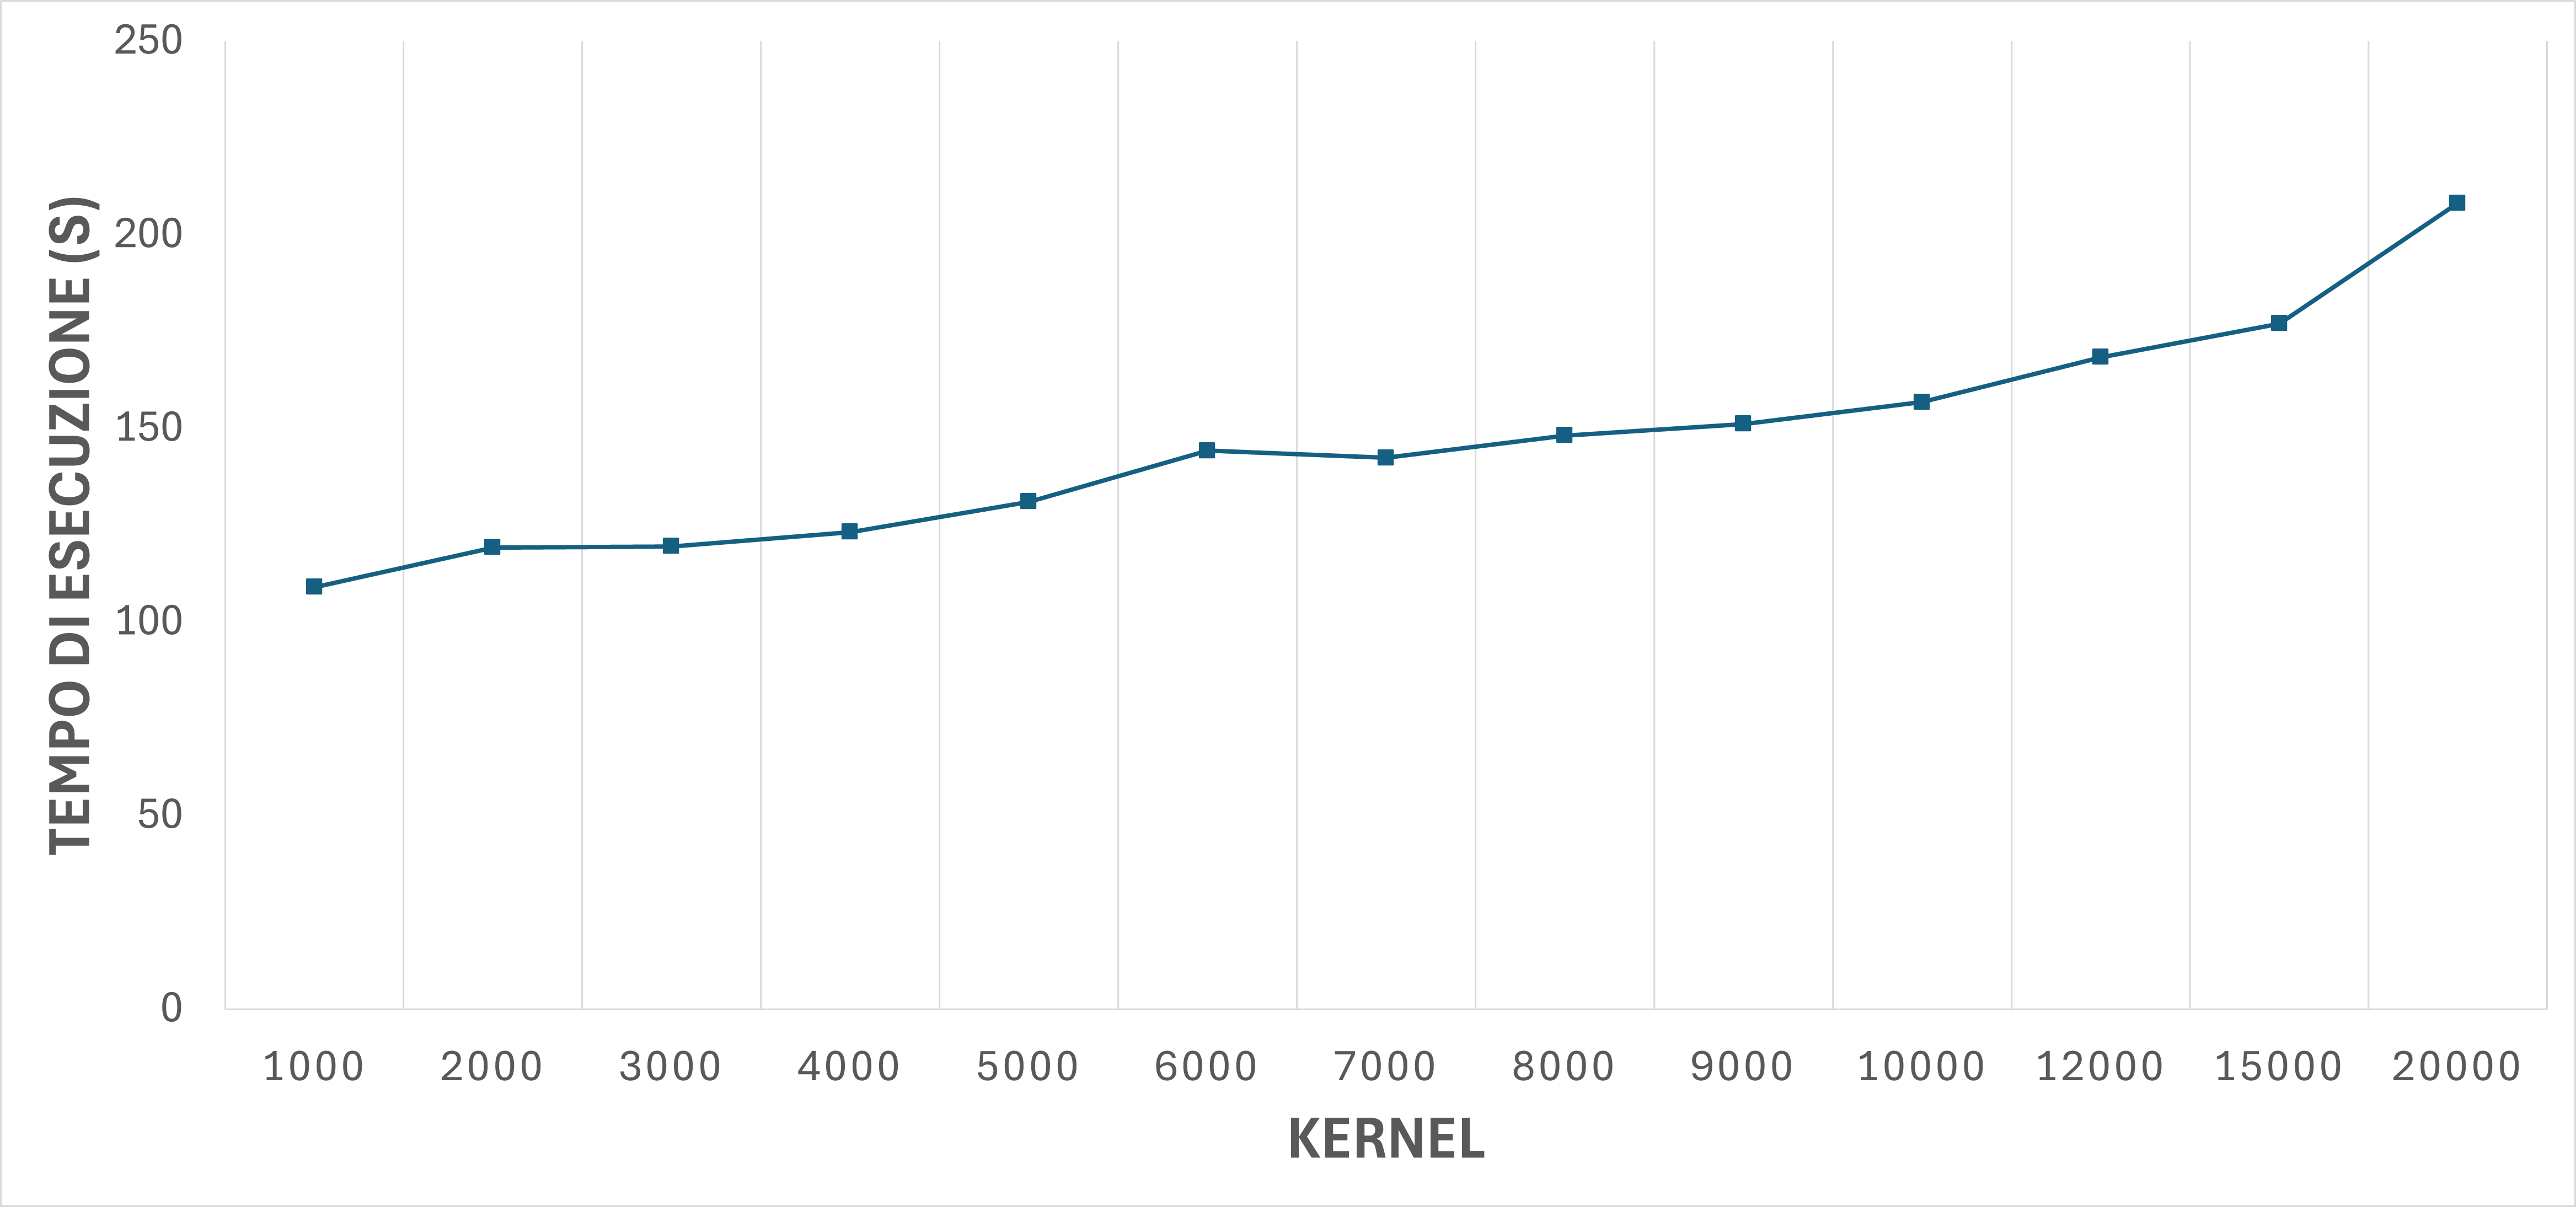
\includegraphics[width=0.9\linewidth]{images//Capitolo7/GraficoTempoEsecuzione_ROCKAD_OPS_SAT.png}
    \caption{Relazione tra F1 e Numero di Kernel - ROCKAD}
    \label{fig:grafico_Tempo_ROCKAD_OPS_SAT}
\end{figure}

Per ottenere questi risultati abbiamo utilizzato gli algoritmi o iperparametri migliori riscontrati nei test precedenti: per ROCKET il classificatore RidgeClassifierCV e per ROCKAD 10 estimatori.
\pagebreak

\section{Risultati Dataset NASA}

Per il dataset NASA, invece, questa situazione si verificava con un numero di kernel pari a 10.000 ed un valore di OFFSET inferiore a 50, questo valore di OFFSET portava con sé anche il problema di non poter aumentare il numero di nodi del KNN, per mancanza di vicini, data la struttura del dataset.

Relativamente alle metriche in questione, analizziamo il grafico in Figura \ref{fig:grafico_f1}, che mostra come cambia la metrica fondamentale, ossia l' F1, con l'aumentare dei kernel.
Nel caso di un numero di kernel pari a 1000 o 10.000 il valore di F1 è pressoché identico, mentre in tutti gli altri valori, la metrica diminuisce significativamente.
Da considerare nell'analisi dobbiamo evidenziare anche il tempo di esecuzione, come mostrato dal grafico nella Figura \ref{fig:grafico_Tempo}, che riporta i tempi di esecuzione dei vari valori dei kernel.

\begin{figure}[!ht]
    \centering
    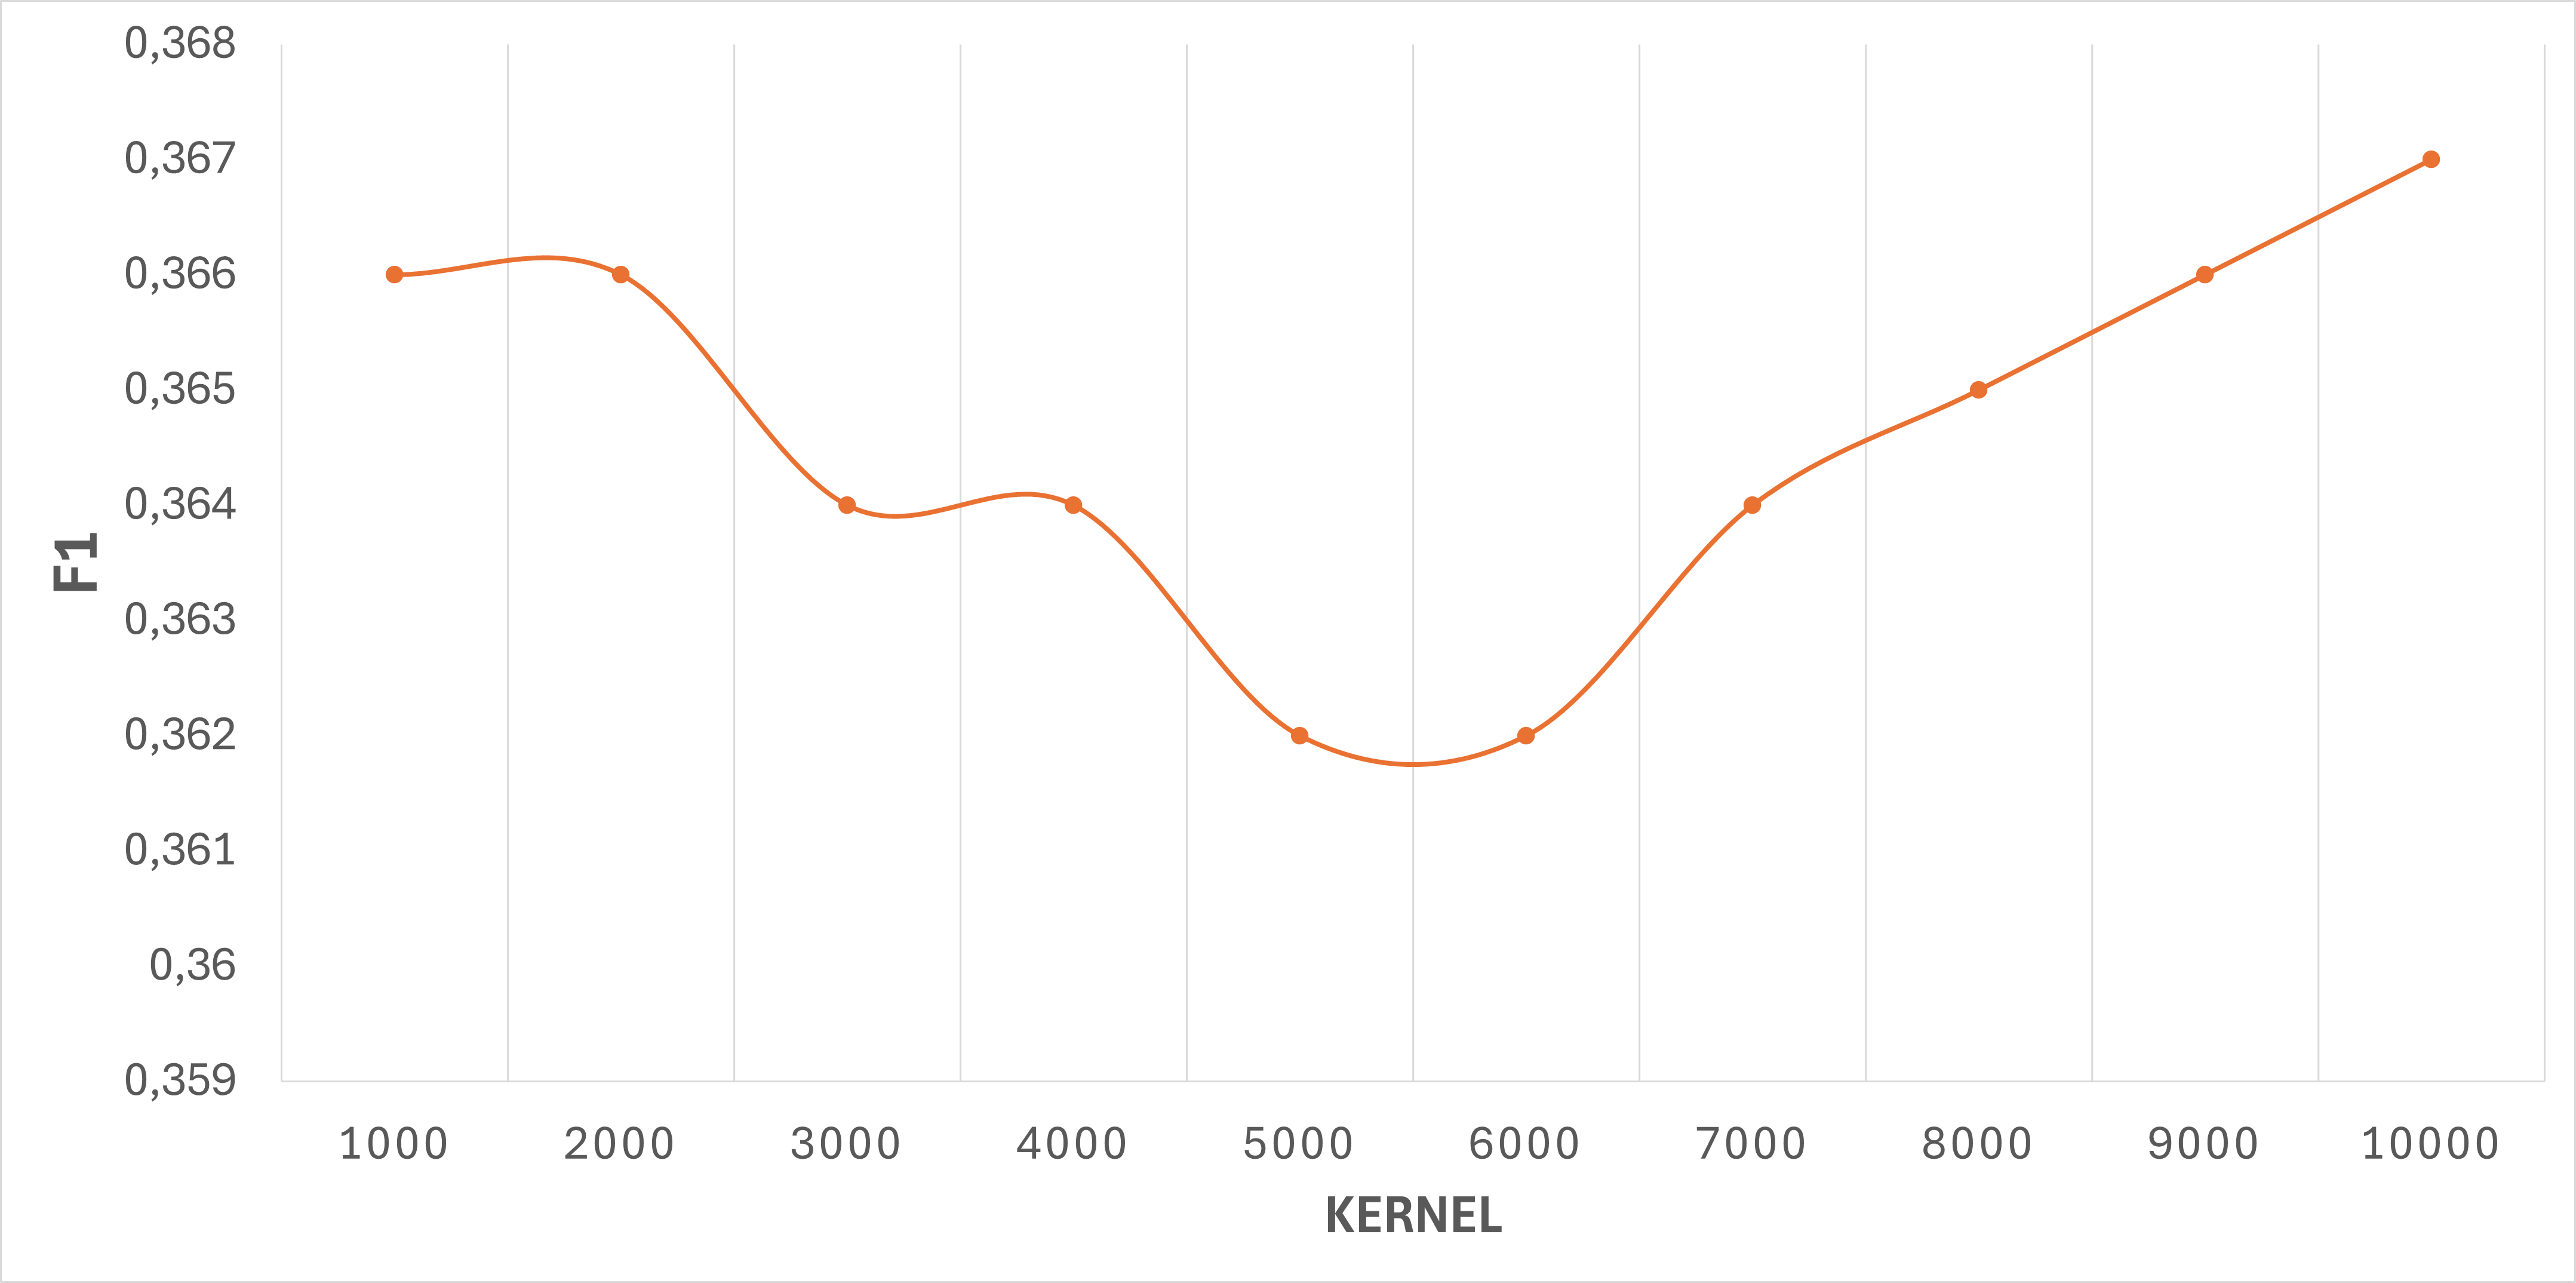
\includegraphics[width=0.9\linewidth]{images//Capitolo7/GraficoF1_ROCKET.png}
    \caption{Relazione tra F1 e Numero di Kernel}
    \label{fig:grafico_f1}
\end{figure}
\begin{figure}[!ht]
    \centering
    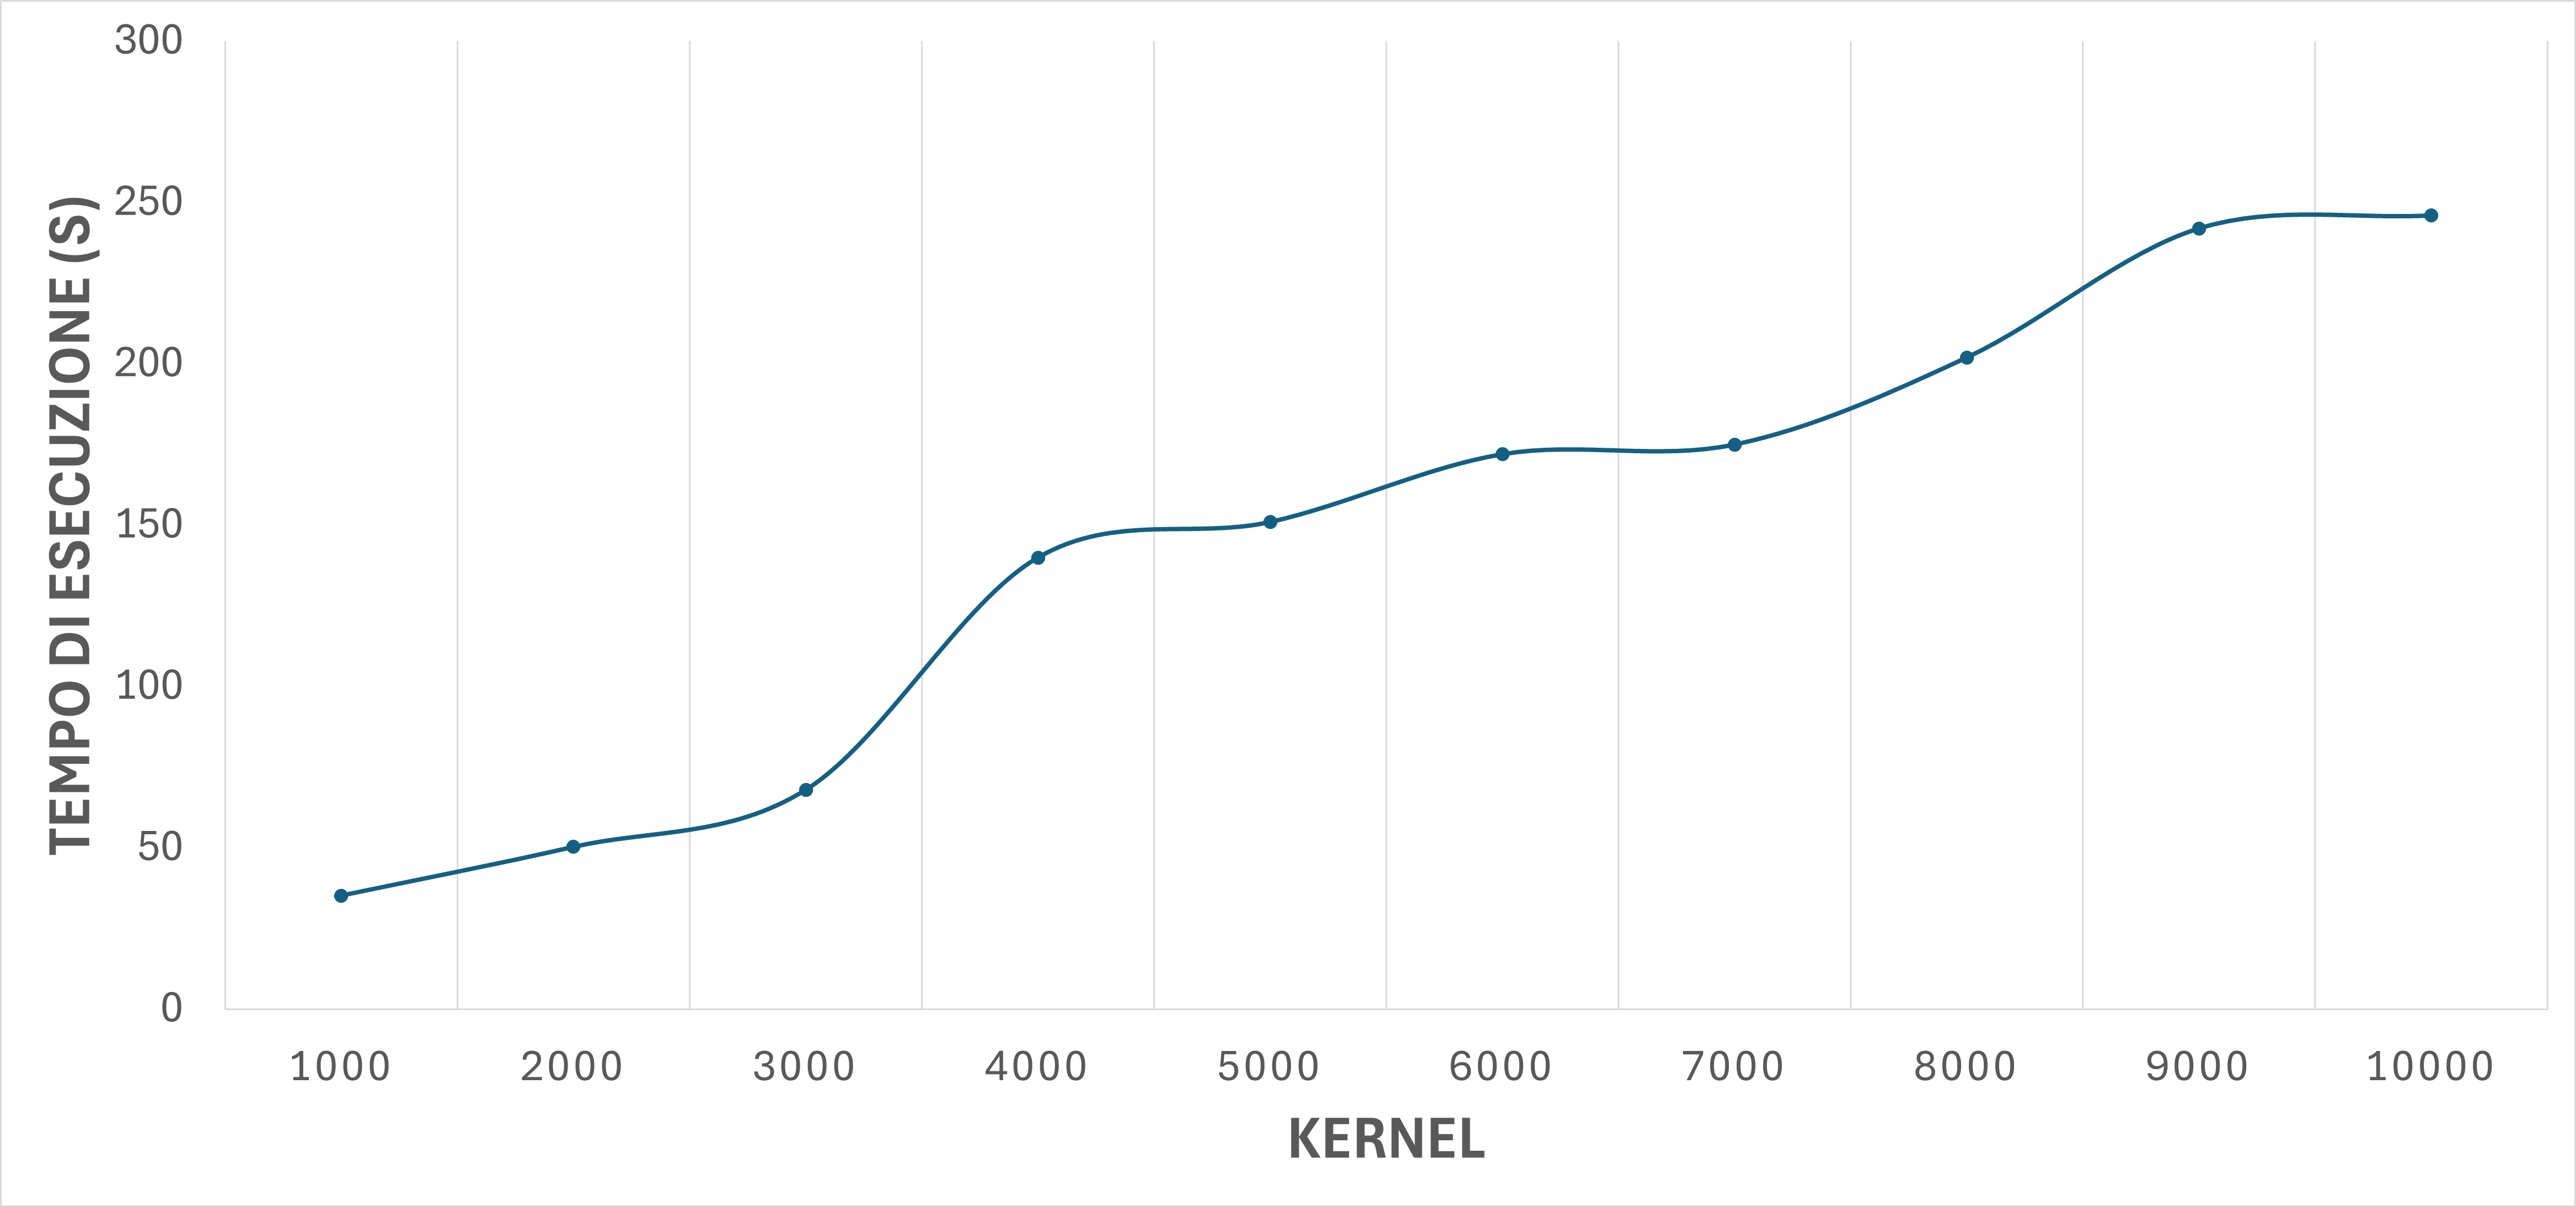
\includegraphics[width=0.9\linewidth]{images//Capitolo7/GraficoTempoEsecuzione_ROCKET.png}
    \caption{Relazione tra Tempi di Esecuzione e Numero di Kernel}
    \label{fig:grafico_Tempo}
\end{figure}
\pagebreak

Da questi grafici possiamo osservare come il tempo di esecuzione aumenti in maniera significativa all'aumentare del numero di kernel, lasciando invariati tutti gli altri parametri. Da questo, evidenziamo meglio che la scelta migliore per il numero di kernel, a parità di valore di F1, è indirizzata verso un valore pari a 1000, dove abbiamo un tempo di esecuzione quasi 7 volte minore rispetto a 10.000. 

Il problema che abbiamo nell'uso di ROCKET, soprattutto su NASA, è proprio quello evidenziato sopra, dato che fissando STEP a 250 l'algoritmo funziona senza troppi problemi e ad una velocità accettabile, ma al diminuire di questo valore il numero di caratteristiche aumenta esponenzialmente portando ad impiegare troppo tempo per fare training e test, non riuscendo a concludere la classificazione. 

Questa riflessione ci permette di capire che il collo di bottiglia di questa metodologia non è direttamente l'applicazione di ROCKET, ma la consecutiva applicazione di un algoritmo di classificazione, che avendo una grande quantità di features, non riesce a gestire in tempi normali.

In merito a ROCKAD, l'analisi della metrica F1 con un numero di kernel variabile tra 1000 e 10.000 è esposta nel grafico in Figura \ref{fig:grafico_f1_ROCKAD}.
Queste misurazioni sono state estratte mantenendo fissati il numero di n\textunderscore neighbors a 2 e OFFSET a 50; notiamo che questo ha un andamento diverso da quanto visto per ROCKET, portando a premiare un numero di kernel compreso tra 3000 e 5000, dove riscontriamo valori più alti di F1.

Il grafico è stato proposto con questi parametri a causa dei problemi relativi ai tempi di esecuzione, infatti nella Tabella \ref{tab:NASA_Posticipato} possiamo vedere come i parametri migliori hanno un OFFSET uguale a 30, ma provando l'esecuzione con quest'ultimo valore, l'algoritmo non terminava in tempi normali.
Infatti a conferma di quanto appena detto, come possiamo vedere dal grafico in Figura \ref{fig:grafico_tempo_ROCKAD}, i tempi di esecuzione, aumentano molto rapidamente fino ad arrivare, nel nostro caso, a più di dieci minuti; questo è stato paragonato con i valori di F1.

\begin{figure}[!ht]
    \centering
    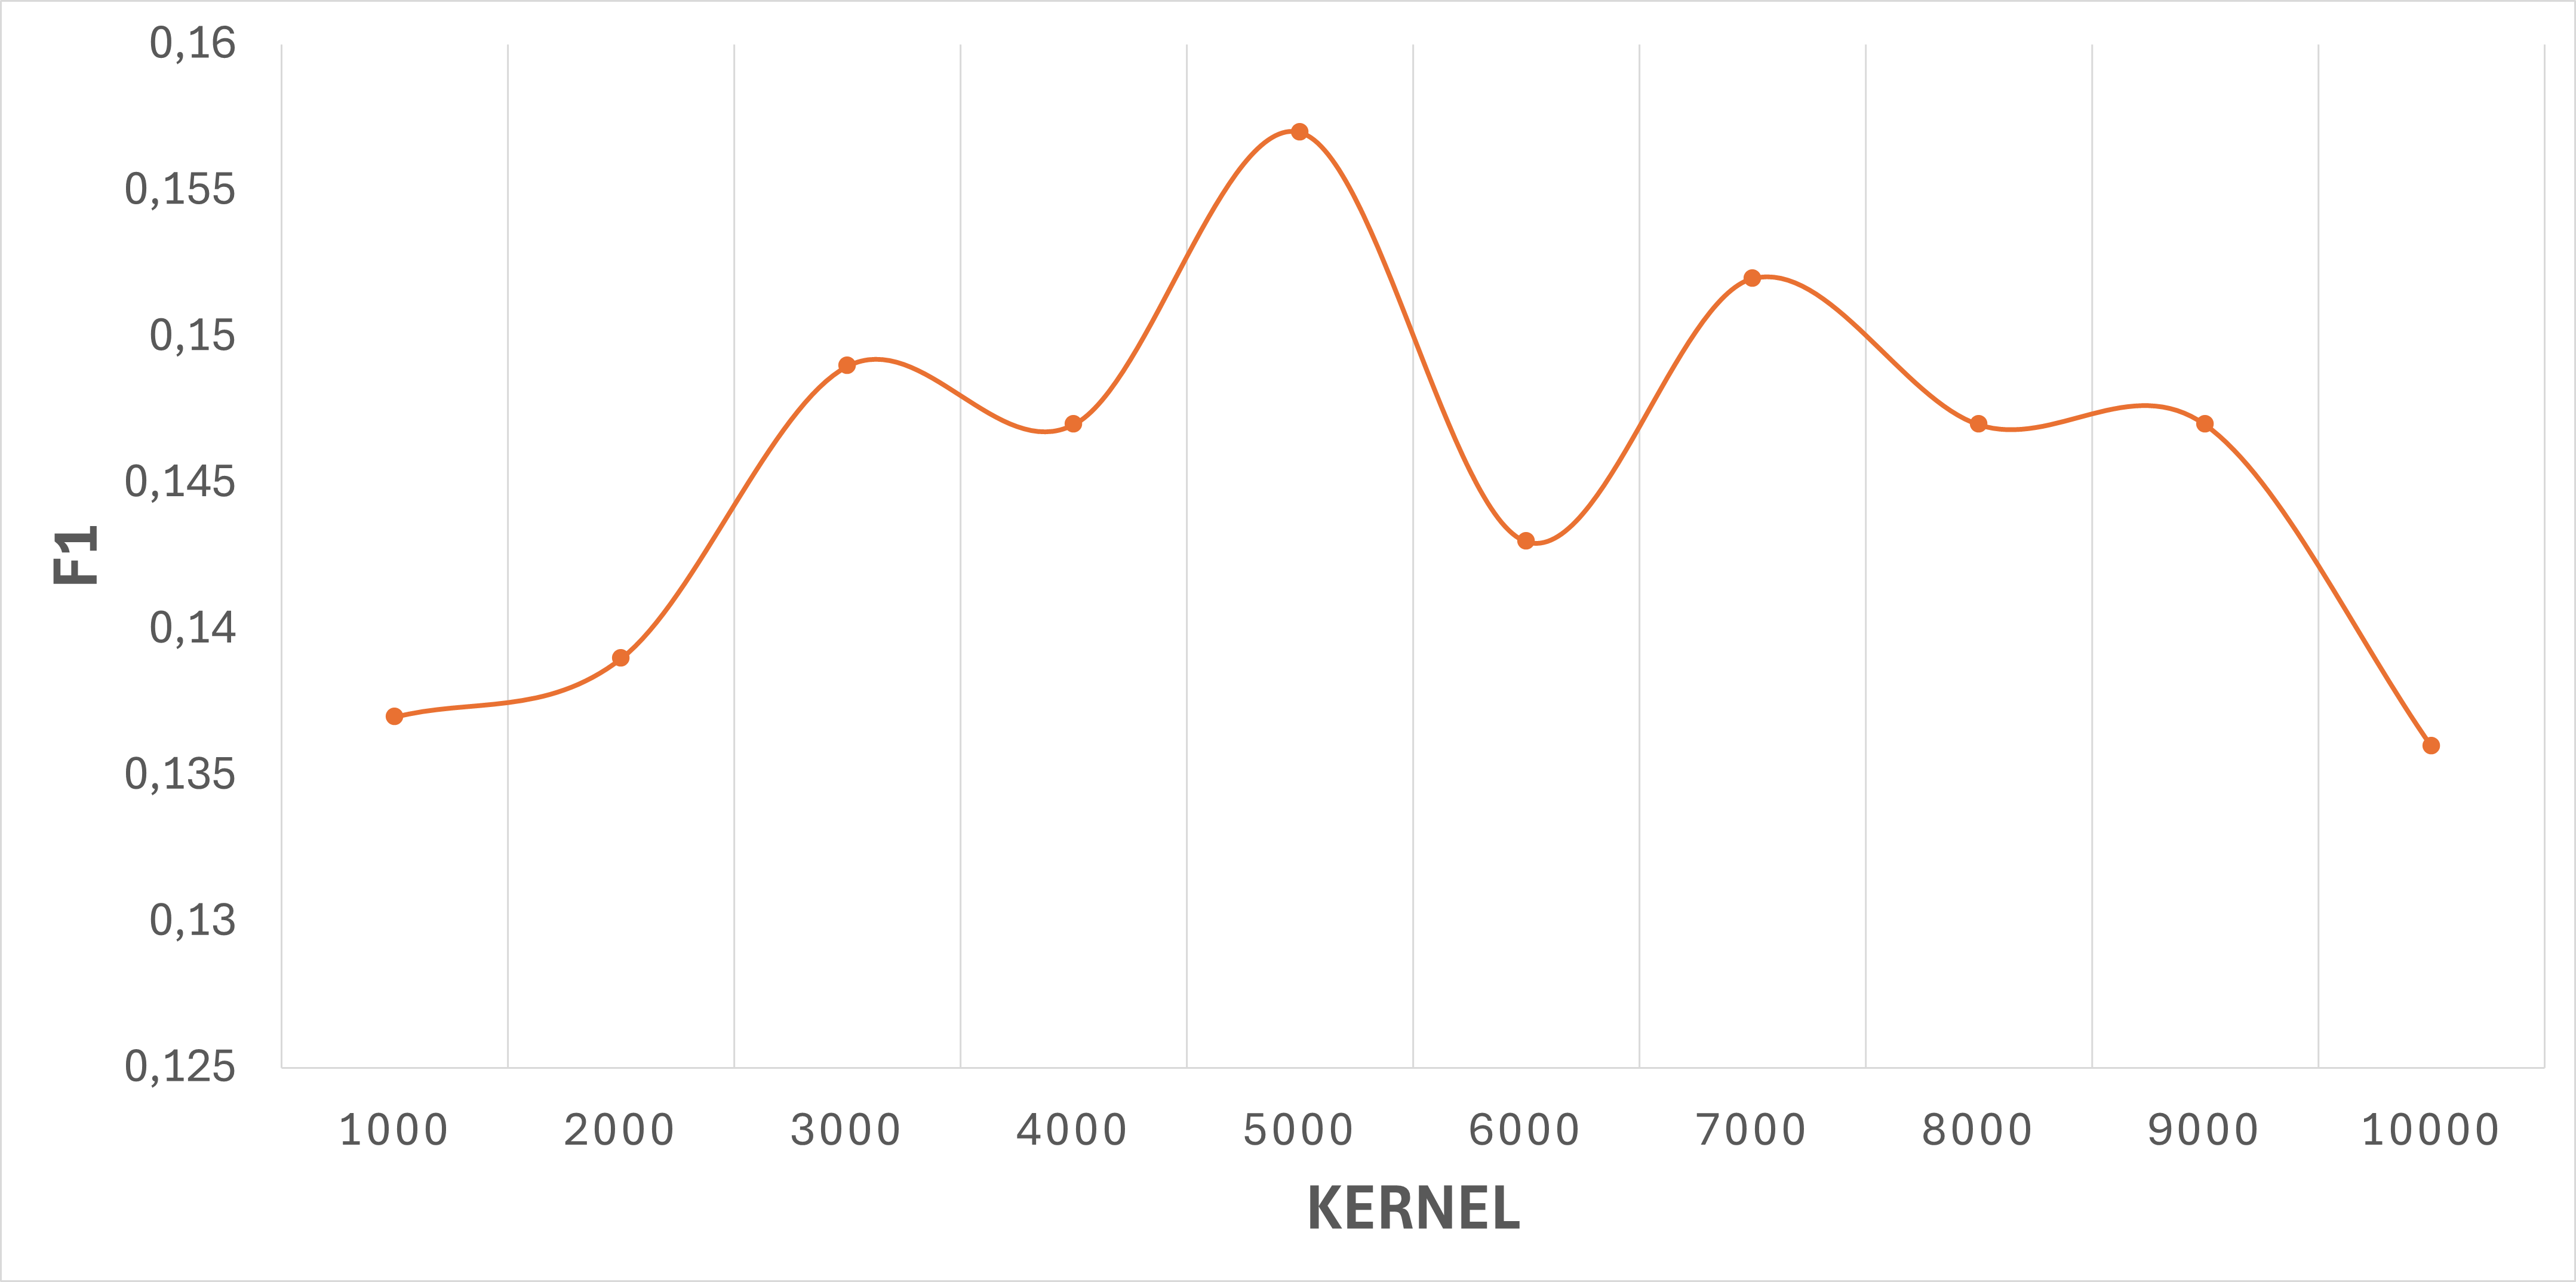
\includegraphics[width=0.9\linewidth]{images//Capitolo7/GraficoF1_ROCKAD.png}
    \caption{Relazione tra F1 e Numero di Kernel}
    \label{fig:grafico_f1_ROCKAD}
\end{figure}

\begin{figure}[!ht]
    \centering
    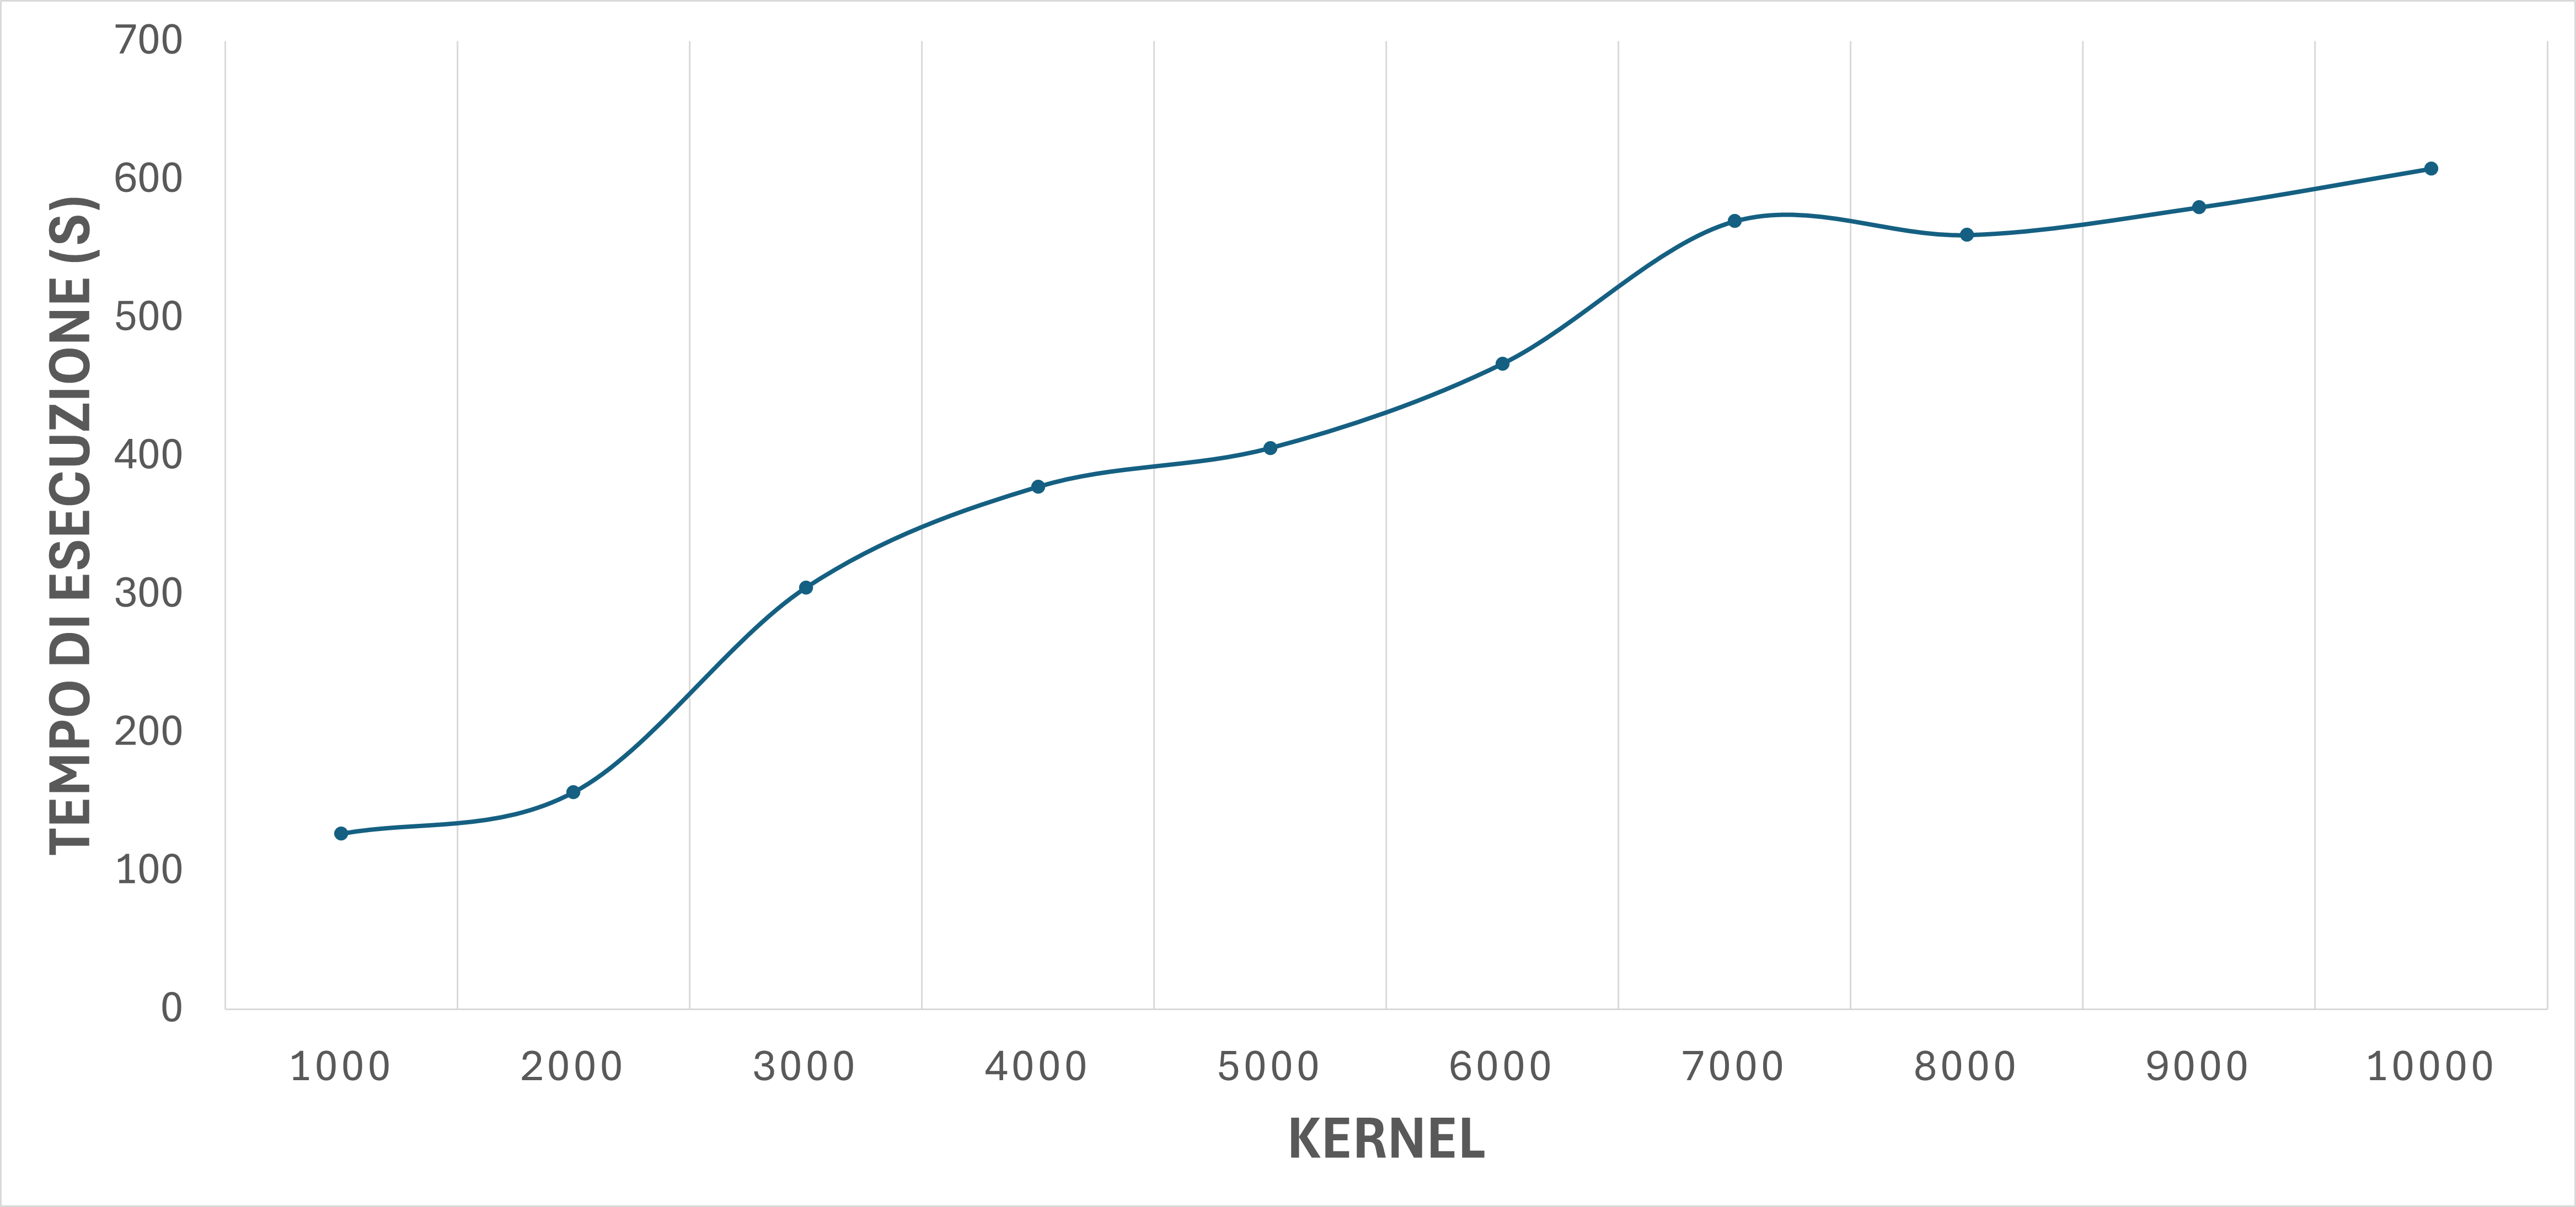
\includegraphics[width=0.9\linewidth]{images//Capitolo7/GraficoTempoEsecuzione_ROCKAD.png}
    \caption{Relazione tra Tempi di Esecuzione e Numero di Kernel}
    \label{fig:grafico_tempo_ROCKAD}
\end{figure}

Analizzando i dati raccolti fino a questo momento, ROCKET si comporta in maniera migliore in tutti i test effettuati, questo lo possiamo osservare dalle metriche, sul dataset OPS\textunderscore SAT, nelle tabelle \ref{tab:RocketOPS_SAT} e \ref{tab:ROCKAD_OPS-SAT}.
Prendendo come metrica di riferimento sempre F1, vediamo che ROCKET ottiene un punteggio di 0.797, invece ROCKAD totalizza 0.634 come picco massimo.

\section{Riflessioni}
Nonostante tutto ciò che è stato discusso precedentemente, l'utilizzo di ROCKET e ROCKAD per il rilevamento delle anomalie risulta un opzione più che valida da poter percorrere, pur rimanendo ancora troppo immatura per essere al pari di soluzioni che utilizzano modelli più comuni, i quali hanno già subito varie iterazioni di miglioramenti, come nel caso di XGBOD.

Come già evidenziato in precedenza, ROCKET e ROCKAD hanno un basso costo computazionale a confronto con modelli più complessi, questo, soprattutto nel contesto satellitare, è un punto critico a causa delle risorse hardware limitate.

ROCKET permette delle performance buone con dataset etichettati e non e potrebbe rivelarsi un buon modello per il rilevamento di anomalie.

ROCKAD, dall'altra parte, permette di essere utilizzato in un ambiente senza etichettatura dei dati e si rivela interessante per i dataset come NASA, oppure, più in generale, in un contesto reale con poche e rare anomalie, spesso non etichettate.

Purtroppo l'applicazione di ROCKAD, risulta ancora poco efficiente, dato soprattutto il suo utilizzo del modello KNN internamente, il quale porta ad una computazione maggiore ed un rischio per la scarsa capacità hardware.

\subsection{Possibili Sviluppi}
Per rendere ROCKET e ROCKAD preferibili ai già consolidati modelli, è necessario apportare ulteriori efficientamenti, così da eguagliare o addirittura superare quelli già esistenti.
Ovviamente questo serve anche per migliorare le attuali performance, già buone in alcuni campi, come l'utilizzo di ROCKET con dataset senza etichettatura.
Elenchiamo di seguito delle possibili proposte per migliorare questi modelli:
\begin{itemize}
    \item Complessità del Modello: ridurre la complessità del modello, data soprattutto dalla generazione di un gran numero di kernel e quindi di caratteristiche; questo può avvenire tramite tecniche di pruning per eliminare le caratteristiche ridondanti o non utili, riducendo la complessità del modello e la possibilità di cadere in overfitting;
    \item Compressione dei Dati: comprimere i dati permette di usarli in modo più efficiente per l'elaborazione, riducendo così anche l'uso della memoria del dispositivo satellitare;
    \item Maggiori Informazioni: data la natura casuale di ROCKET, i pattern non sono analizzabili esternamente, portando ad un limite nell'interpretazione e comprensione delle caratteristiche; migliorando questo aspetto, tramite ad esempio strumenti di visualizzazione, potrebbe portare ad un miglioramento nell'analisi dei risultati;
    \item Validazione: l'ultimo aspetto, dopo aver effettuato tutte le migliorie possibili, sarebbe l'applicazione di questi modelli in un contesto reale per validarne l'efficacia e l'efficienza, questo potrebbe avvenire, ad esempio, sulla nuova missione OPS\textunderscore SAT programmata per la fine di questo anno.
\end{itemize}

\chapter{Conclusioni}
% Riportare dati dei tre algoritmi XGBOD, ROCKET e ROCKAD
% Supervised si comportano meglio di quelli Unsupervised
% Con NASA  i risultati sono ancora migliorabili ma ROCKET è una soluzione che potrebbe essere promettente soprattutto per il fatto che aumenta il numero di caratteristiche con un costo computazionale relativamente contenuto
% Bisogna però trovare il compromesso tra complessità e performance
% ROCKET è utilizzabile per anomaly detection? -> Si ma bisogna rendere più ottimizzata l'esecuzione soprattutto con un numero maggiore di kernel, questo però soprattutto per l'esecuzione con NASA che richiede molto tempo
% Su OPS_SAT l'esecuzione è molto più rapida per ROCKET

%---- FORSE AGGIUNGERE TEMPI ESECUZIONE ROCKET E ROCKAD su OPS_SAT ----

In questo documento abbiamo analizzato ed esplorato nuovi approcci per il rilevamento di anomalie, proponendoci di sperimentare nuove metodologie in quest'ambito, cercando di fornire più informazioni possibili per i futuri ricercatori che vorranno approfondire l'utilizzo di ROCKET, così da agevolare in tal senso il suo utilizzo.
Lo scopo di questo documento è incentrato anche sull'analisi delle performance e della possibilità di utilizzare questi algoritmi in contesti reali.

Il lavoro inizialmente è stato effettuato sul dataset OPS\textunderscore SAT dell'ESA, che ci ha permesso un accesso facilitato alla sperimentazione e allo sviluppo di tecniche di rilevamento delle anomalie.
Successivamente, siamo passati a lavorare sul dataset NASA, testando i modelli in questione sotto vari valori degli iperparametri, confrontando prestazioni ed efficienza in ognuno, in un contesto più ampio e realistico.

Da questi test e dalle successive analisi dei dati ottenuti, è stato possibile rilevare che l'efficienza di ROCKET e ROCKAD è dipendente dal valore assegnato a STEP (la lunghezza delle sotto sequenze della timeseries); questo valore è particolarmente importante, soprattutto sul dataset OPS\textunderscore SAT, poiché da esso dipende la velocità di esecuzione.
Allo stesso modo, per il dataset NASA, l'efficienza dipende strettamente dal valore di OFFSET, che permette l'overlapping (sovrapposizione di segmenti consecutivi per aumentare il numero di sotto sequenze).
In particolare, osserviamo che fissando il numero di kernel a 10.000, i valori di STEP inferiori a 250 sono sconsigliati, mentre valori di OFFSET inferiori a 50 portano ad un aumento esponenziale del tempo di esecuzione, oltre ad una classificazione peggiore rispetto a tali valori.
Bisogna anche menzionare il problema relativo alla classificazione riguardante il dataset NASA: con un valore di OFFSET maggiore di quello indicato, potrebbe portare ad una mancanza di nodi vicini per il classificatore KNN.

Per il dataset OPS\textunderscore SAT, gli iperparametri migliori risultanti dai nostri test risultano essere:
\begin{enumerate}
    \item XGBOD: il miglior risultato è stato ottenuto tramite la modalità che utilizza più modelli, ossia KNN, LOF, ABOD e OCSVM e con i seguenti parametri n\textunderscore estimators=100, max\textunderscore depth=3 e learning\textunderscore rate=0.2;
    \item ROCKET: i risultati ottimali risultano essere con un numero di kernel uguale a 10.000 e l'utilizzo del classificatore supervised RidgeClassifierCV;
    \item ROCKAD: con un numero di kernel pari a 10.000 e un numero di estimatori uguale a 10, siamo riusciti ad ottenere il miglior risultato, sia per tempo di esecuzione che per metriche riscontrate.
\end{enumerate}

Per quanto riguarda il dataset NASA e considerando ROCKET con un numero di kernel pari a 1000 o 10.000, un numero di vicini uguale ad 1 ed un OFFSET di 50 otteniamo un buon rapporto tra accuratezza e velocità di esecuzione.
Questi risultati ci fanno ben sperare nell'applicazione futura di questo modello per il rilevamento delle anomalie, soprattutto in merito al suo utilizzo in maniera supervised, con dati etichettati, dato il suo basso costo computazionale e la capacità di rilevare correttamente la maggior parte delle anomalie.

Non possiamo affermare le stesse conclusioni per ROCKAD, che ha dimostrato varie limitazioni relative al costo computazionale più elevato rispetto a ROCKET, questo porta spesso ad un tempo di esecuzione molto elevato che non si rispecchia però in metriche altrettanto buone.
Tramite i test effettuati, i miglior risultati sono stati ottenuti con 1000 kernel, 2 vicini e un OFFSET pari a 30, portando così ad avere un numero di caratteristiche estratte inferiori, conservando metriche uguali ed un tempo di esecuzione nettamente migliore, rispetto ad avere 10.000 kernel.
ROCKAD rimane comunque consigliato nell'utilizzo con dati non etichettati, a causa della sua implementazione.

Questo documento ci apre la strada verso nuove ricerche future.
Sicuramente è di fondamentale importanza concentrarsi sull'ottimizzazione di questi algoritmi, esplorando ulteriormente i parametri per ridurre il più possibile i tempi di esecuzione.
Un altro aspetto da considerare, soprattutto per l'utilizzo sui satelliti, è l'efficientamento. Questo può avvenire tramite tecniche di Transfer Learning e Fine-Tuning, così da rendere i modelli più leggeri da utilizzare.

Il passo successivo è l'utilizzo degli algoritmi su altri dataset, testando le prestazioni e valutandone la robustezza in contesti diversi.
Questi risultati servono come punto di partenza per avere dei valori di riferimento degli algoritmi con cui validare o confrontare metodi nuovi.

Il documento rappresenta un contributo nell'ambito del rilevamento delle anomalie, fornendo un primo passo verso la comprensione delle potenzialità e delle limitazioni degli algoritmi ROCKET, ROCKAD e XGBOD per l'utilizzo a bordo dei satelliti.
I risultati forniscono una base per lo sviluppo ulteriore di sistemi di monitoraggio più efficienti e affidabili per le missioni satellitari, con particolare attenzione all'ottimizzazione del consumo delle risorse dei satelliti.
% Mamma e Babbo
% Alberto e Cinzia
% Giada
% Nonni

% In dubbio Relatore e Correlatore
\chapter*{Ringraziamenti}

Alla fine di questo percorso, sento il dovere di dedicare questo spazio per ringraziare tutte le persone che, in questi anni, mi hanno aiutato e sostenuto in tutto il percorso universitario e personale.


% Primo nel caso va il relatore e correlatore

Ovviamente un grande ringraziamento va ai miei genitori, che durante questi anni mi hanno sostenuto ad andare avanti, a migliorarmi sempre di più, senza chiedere mai nulla in cambio.
Tutto questo, nonostante spesso si ritrovassero un muro contro cui scontrarsi, che non ascolta e continua della sua idea, ma non hanno mai smesso di provare, insistere e cercare di oltrepassare quel muro, non per un loro tornaconto, ma per darmi il migliore futuro possibile.
Non mi hanno mai fatto mancare nulla, parlando, discutendo e litigando per ogni mio capriccio, per ogni mia richiesta folle che per me, in quel momento, era essenziale, ma che in realtà mi distoglieva solo dall'obbiettivo finale.

Grazie a Mamma e Babbo ho potuto trascorrere il tempo universitario senza avere fretta di concludere tutto, senza mai pressioni, facendomi trascorrere questi anni in "tranquillità", si fa per dire ovviamente.

Non posso non ringraziare anche mio fratello, che durante questi anni è sempre stato il primo a spronarmi a fare sempre meglio e sempre di più; nonostante le litigate, le incomprensioni e i rimproveri, non so se sarei riuscito a finire l'università in pari senza i suoi consigli e le sue indicazioni.

Un grande ringraziamento va anche a Cinzia che, da quando è entrata in casa, l'ho sempre considerata come una sorella, con la quale poter parlare e confrontarmi su ogni aspetto; alla quale poter sempre chiedere un opinione o un consiglio senza essere mai giudicato.

Un pensiero speciale va anche ai miei nonni, che mi hanno sempre motivato ad andare avanti ed proseguire gli studi; mi hanno sempre ascoltato quando un esame andava male e avevo bisogno di parlare.

Infine un enorme ringraziamento va anche a Giada. Ormai stiamo insieme da due anni e mezzo e sono sicuro che, se non l'avessi incontrata, sarei una persona diversa.
Durante tutto il percorso mi è stata accanto, incentivandomi a continuare a studiare anche quando tutto sembrava inutile. Ha sopportato e continuato ad ascoltarmi innumerevoli volte, aiutandomi durante tutta la stesura della tesi.
Mi ricorderò sempre le chiamate per svegliarci a vicenda e per darci la forza di studiare, le serate prima degli esami a disperarci pensando di avere la sicurezza di bocciare, tra un momento di ripasso ed uno d'ansia, e il cornetto dopo ogni esame passato o bocciato per tirarci un po' su di morale.

A tutte le persone che ci sono state e ci sono ancora vi ringrazio di cuore.
% \begin{table}[h!]
    \centering % Correttamente posizionato
    \begin{adjustbox}{max width=\textwidth}
        \begin{tabular}{|c|c|c|c|c|c|c|c|c|c|}
        \hline
        \textbf{Modalità} & \textbf{Accuracy} &\textbf{Precision}  & \textbf{Recall} & \textbf{F1} & \textbf{MCC} & \textbf{AUC-PR} & \textbf{AUC-ROC} & \textbf{NScore}&\textbf{Tempo}\\
        \hline
        \multicolumn{10}{|c|}{\textbf{ROCKET}} \\
        \hline
         \textbf{RidgeCV} &\textbf{ 0.777} & 0.704 & \textbf{0.919} &\textbf{0.797}  & \textbf{0.584} & 0.787& 0.829 &0.726&6.6s \\
        \hline
        \textbf{LogisticReg} & \textbf{0.777} & 0.704 & \textbf{0.919} &\textbf{0.797}  &\textbf{ 0.584} & 0.773& 0.837 &\textbf{0.774} &53.3s\\
        \hline
        \multicolumn{10}{|c|}{\textbf{ROCKAD}} \\
        \hline
        (10,10.000)&\textbf{0.546} &\textbf{0.515} &\textbf{0.823} &\textbf{0.634} & \textbf{0.137}& 0.757& 0.704&0.677& 2m 12.5s\\
        \hline
        (30,10.000)&0.508 &0.489 &0.71 &0.579 &0.036 &\textbf{0.762} &\textbf{0.709}& 0.677& 3m 17.1s\\
        \hline
        \end{tabular}
    \end{adjustbox}
    \caption{ROCKET e ROCKAD su dataset OPS\textunderscore SAT}
    \label{tab: ROCKET_ROCKAT_OPS_SAT}
\end{table}


% TEST SU NASA ===========

\begin{table}[!ht]
    \centering % Correttamente posizionato
    \begin{adjustbox}{max width=\textwidth}
        \begin{tabular}{|c|c|c|c|c|c|c|c|}
        \hline
        \textbf{Accuracy} &\textbf{Precision}  & \textbf{Recall} & \textbf{F1} & \textbf{MCC} & \textbf{AUC-PR} & \textbf{AUC-ROC} & \textbf{NScore}\\
        \hline
        \multicolumn{8}{|c|}{\textbf{ROCKET}} \\
        \hline
        \multicolumn{8}{|c|}{kernel=10.000, n\textunderscore neighbors=1 e OFFSET=50} \\
        \hline
         \textbf{0.735} & \textbf{0.299} & 0.471 &0.366  & \textbf{0.232 }& 0.286& 0.652 & 0.378 \\
        \hline
        \multicolumn{8}{|c|}{kernel=1000, n\textunderscore neighbors=1 e OFFSET=50} \\
        \hline
         0.731 & 0.296 & 0.478 &\textbf{0.367}  & 0.231 & \textbf{0.288}& \textbf{0.654} & \textbf{0.384} \\
        \hline
        \multicolumn{8}{|c|}{kernel=1000, n\textunderscore neighbors=5 e OFFSET=10} \\
        \hline
         0.730 & 0.295 & 0.477 &0.365  & 0.230 & 0.278& 0.648 & 0.382 \\
         \hline
        \multicolumn{8}{|c|}{\textbf{ROCKAD}} \\
        \hline
        \multicolumn{8}{|c|}{kernel=10.000, n\textunderscore neighbors=2 e OFFSET=30} \\
        \hline
        0.628 & \textbf{0.131} & 0.207 &0.16  & \textbf{-0.076} &\textbf{0.29} &0.646  &0.379 \\
        \hline
        \multicolumn{8}{|c|}{ROCKAD con 1000 kernel, n\textunderscore neighbors=2 e OFFSET=30} \\
        \hline
        0.614 & 0.129 & \textbf{0.218} &\textbf{0.162}  & -0.083 &\textbf{0.29} &0.646  &\textbf{0.381} \\
        \hline
        \end{tabular}
    \end{adjustbox}
    \caption{ROCKET e ROCKAD su dataset NASA}
    \label{tab:ROCKET_ROCKAD_NASA}
\end{table}
% \appendix

% \include{chapters/AppendiceA}

\bibliography{chapters/Bibliografia.bib}

\end{document}
% -----------------------------------------------------------------
